%File: anonymous-submission-latex-2023.tex
\documentclass[letterpaper]{article}
% \usepackage[submission]{aaai23}  % DO NOT CHANGE THIS
\usepackage{aaai23}  % DO NOT CHANGE THIS
\usepackage{times}  % DO NOT CHANGE THIS
\usepackage{helvet}  % DO NOT CHANGE THIS
\usepackage{courier}  % DO NOT CHANGE THIS
\usepackage[hyphens]{url}  % DO NOT CHANGE THIS
\usepackage{graphicx} % DO NOT CHANGE THIS
\urlstyle{rm} % DO NOT CHANGE THIS
\def\UrlFont{\rm}  % DO NOT CHANGE THIS
\usepackage{natbib}  % DO NOT CHANGE THIS AND DO NOT ADD ANY OPTIONS TO IT
\usepackage{caption} % DO NOT CHANGE THIS AND DO NOT ADD ANY OPTIONS TO IT
\frenchspacing  % DO NOT CHANGE THIS
\setlength{\pdfpagewidth}{8.5in} % DO NOT CHANGE THIS
\setlength{\pdfpageheight}{11in} % DO NOT CHANGE THIS
%
% Keep the \pdfinfo as shown here. There's no need
% for you to add the /Title and /Author tags.
\pdfinfo{
/TemplateVersion (2023.1)
}

% These are recommended to typeset algorithms but not required. See the subsubsection on algorithms. Remove them if you don't have algorithms in your paper.
\usepackage{algorithm}
\usepackage{algorithmic}

\usepackage{cite}
\usepackage{amsmath,amssymb,amsfonts,amsthm}
\usepackage{mathrsfs}

%
% These are are recommended to typeset listings but not required. See the subsubsection on listing. Remove this block if you don't have listings in your paper.
% \usepackage{newfloat}
\usepackage{listings}
\DeclareCaptionStyle{ruled}{labelfont=normalfont,labelsep=colon,strut=off} % DO NOT CHANGE THIS
\lstset{%
	basicstyle={\footnotesize\ttfamily},% footnotesize acceptable for monospace
	numbers=left,numberstyle=\footnotesize,xleftmargin=2em,% show line numbers, remove this entire line if you don't want the numbers.
	aboveskip=0pt,belowskip=0pt,%
	showstringspaces=false,tabsize=2,breaklines=true}
\floatstyle{ruled}
\newfloat{listing}{tb}{lst}{}
\floatname{listing}{Listing}

\usepackage{graphicx}
\usepackage{textcomp}
\usepackage{xcolor}
% \def\BibTeX{{\rm B\kern-.05em{\sc i\kern-.025em b}\kern-.08em
%     T\kern-.1667em\lower.7ex\hbox{E}\kern-.125emX}}

\usepackage{comment}
\usepackage{xparse}
% \usepackage{amsmath,amsfonts,amssymb,amsthm}
\usepackage{mathtools}
\usepackage{subcaption}
\usepackage{enumerate}

\newcommand{\toolname}{\textsc{Mungojerrie} }

\usepackage{xparse}
\usepackage{mathtools}
\usepackage{tikz}
\usepackage{subcaption}
\usepackage{enumerate}
% \renewcommand\labelitemi{--}

\newtheorem{theorem}{Theorem}[]
\newtheorem{example}{Example}[]
\newtheorem{corollary}[theorem]{Corollary}
\newtheorem{lemma}[theorem]{Lemma}
\newtheorem{problem}[theorem]{Problem}

\usepackage{paralist}
\usepackage{todonotes}
\definecolor{purple}{rgb}{1, 0, 1}

\newcommand{\ie}{\emph{i.e.,}\xspace}
\newcommand{\eg}{\emph{e.g.,}\xspace}
\newcommand{\abr}{\emph{abbr.}\xspace}
\newcommand{\ea}{\emph{et al.}\xspace}
\newcommand{\gensync}{\emph{GenSync}\xspace}
\newcommand{\colosseum}{\emph{Colosseum}\xspace}
\newcommand{\srep}{\emph{SREP}\xspace} % Set Reconciliation Enhances
\newcommand{\srepsim}{\emph{SREPSim}\xspace}
% Propagation
\newcommand{\esrep}{\emph{E-SREP}\xspace}
\newcommand{\epsrep}{\emph{EP-SREP}\xspace}
\newcommand{\mesrep}{\emph{ME-SREP}\xspace}
\newcommand{\mempoolsync}{\emph{MempoolSync}}

\newcommand{\fref}[1]{Fig.~\ref{#1}}
\newcommand{\tref}[1]{Table~\ref{#1}}
\newcommand{\aref}[1]{Algorithm~\ref{#1}}
\newcommand{\procref}[1]{Procedure~\ref{#1}}
\newcommand{\sref}[1]{Section~\ref{#1}}
\newcommand{\lineref}[1]{line~\ref{#1}}
\newcommand{\appref}[1]{Appendix~\ref{#1}}

% Change \eqref
\LetLtxMacro{\originaleqref}{\eqref}
\renewcommand{\eqref}{Eq.~\originaleqref}

% Theorems and corollaries
\newcounter{theoremcount}
\setcounter{theoremcount}{0}
\DeclareRobustCommand{\theorem}[1]{%
  \refstepcounter{theoremcount}%
  \noindent\textit{\textbf{Theorem \thetheoremcount\label{theorem:#1}: }}%
}
\DeclareRobustCommand{\theoremref}[1]{Theorem~\ref{theorem:#1}}

\DeclareRobustCommand{\proof}{\emph{Proof:}\xspace}
\DeclareRobustCommand{\qqed}{\hfill$\blacksquare$}

\newcounter{corollcount}
\setcounter{corollcount}{0}
\DeclareRobustCommand{\coroll}[1]{%
  \refstepcounter{corollcount}%
  \noindent\textit{\textbf{Corollary \thecorollcount\label{coroll:#1}: }}%
}
\DeclareRobustCommand{\corollref}[1]{Corollary~\ref{coroll:#1}}

\newcounter{lemmacount}
\setcounter{lemmacount}{0}
\DeclareRobustCommand{\lemma}[1]{%
  \refstepcounter{lemmacount}%
  \noindent\textit{\textbf{Lemma \thelemmacount\label{lemma:#1}: }}%
}
\DeclareRobustCommand{\lemmaref}[1]{Lemma~\ref{lemma:#1}}

\newcounter{definitioncount}
\setcounter{definitioncount}{0}
\DeclareRobustCommand{\definition}[1]{%
  \refstepcounter{definitioncount}%
  \noindent\textit{\textbf{Definition \thedefinitioncount\label{definition:#1}: }}%
}
\DeclareRobustCommand{\defref}[1]{Definition~\ref{definition:#1}}

%notes of different authors
\newif\ifnotes
\notestrue
\notesfalse

\newif\ifdiff
\difftrue
\difffalse

\newcommand{\anote}[1]{\ifnotes $\ll$\textsf{\textcolor{purple}{Ari: {#1}}}$\gg$ \fi}
\newcommand{\nnote}[1]{\ifnotes $\ll$\textsf{\textcolor{orange}{Novak: {#1}}}$\gg$ \fi}
\newcommand{\diff}[1]{\ifdiff\textcolor{orange}{#1}\else#1\fi}

%%% Local Variables:
%%% mode: latex
%%% TeX-master: "main"
%%% End:


\usetikzlibrary{automata,positioning,decorations.markings,arrows,intersections,%    
calc,shapes,fit}                                     
\colorlet{darkgreen}{green!40!black}                                                                   \colorlet{darkblue}{blue!60!black}                                                                     \colorlet{darkred}{red!50!black}                                                                       \colorlet{safecellcolor}{yellow!5}                                                                     \colorlet{goodcellcolor}{green!10}                                                                     \colorlet{badcellcolor}{blue!10}      

% \usetikzlibrary{automata, arrows.meta,arrows, positioning}

\tikzset{
    >=latex,node distance=2cm,on grid,auto, initial text=, 
    box state/.style={draw,rectangle,minimum size=8mm,rounded corners},
    prob state/.style={draw,very thick,shape=circle,darkblue,minimum size=3mm,inner sep=0mm},
    every loop/.style={shorten >=0pt},
    accepting state/.style={double distance=1.2pt, outer sep = 0.6pt+\pgflinewidth},
    accepting dot/.style={above=-2.7pt,circle,fill,darkgreen,inner sep=2pt,radius=1pt}, 
    loop above/.append style={every loop/.append style={out=120, in=60, looseness=6}},
    loop below/.append style={every loop/.append style={out=300, in=240, looseness=6}},
    loop left/.append style={every loop/.append style={out=210, in=150, looseness=6}},
    loop right/.append style={every loop/.append style={out=30, in=330, looseness=6}} 
}  

% % Number the lines for submission
% \usepackage[mathlines]{lineno}
% \setlength\linenumbersep{0.5cm}
% \renewcommand\thelinenumber{\color{red!80!black}\arabic{linenumber}~}
% \let\oldqed\qed
% \renewcommand\qed{\mbox{}\hfill$\oldqed$}
% \newcommand*\patchAmsMathEnvironmentForLineno[1]{%
%   \expandafter\let\csname old#1\expandafter\endcsname\csname #1\endcsname
%   \expandafter\let\csname oldend#1\expandafter\endcsname\csname end#1\endcsname
%   \renewenvironment{#1}%
%   {\linenomath\csname old#1\endcsname}%
%   {\csname oldend#1\endcsname\endlinenomath}}% 
% \newcommand*\patchBothAmsMathEnvironmentsForLineno[1]{%
%   \patchAmsMathEnvironmentForLineno{#1}%
%   \patchAmsMathEnvironmentForLineno{#1*}}%
% \AtBeginDocument{%
%   \patchBothAmsMathEnvironmentsForLineno{equation}%
%   \patchBothAmsMathEnvironmentsForLineno{align}%
%   \patchBothAmsMathEnvironmentsForLineno{flalign}%
%   \patchBothAmsMathEnvironmentsForLineno{alignat}%
%   \patchBothAmsMathEnvironmentsForLineno{gather}%
%   \patchBothAmsMathEnvironmentsForLineno{multline}%
% }
% \linenumbers
% remove the above for final version


\DeclareCaptionStyle{ruled}{labelfont=normalfont,labelsep=colon,strut=off} % DO NOT CHANGE THIS
\frenchspacing  % DO NOT CHANGE THIS
\setlength{\pdfpagewidth}{8.5in}  % DO NOT CHANGE THIS
\setlength{\pdfpageheight}{11in}  % DO NOT CHANGE THIS
%
% These are recommended to typeset algorithms but not required. See the subsubsection on algorithms. Remove them if you don't have algorithms in your paper.
\usepackage{algorithm}
\usepackage{algorithmic}
\usepackage{temporal}
%
% These are are recommended to typeset listings but not required. See the subsubsection on listing. Remove this block if you don't have listings in your paper.
\usepackage{newfloat}
\usepackage{listings}
\lstset{%
	basicstyle={\footnotesize\ttfamily},% footnotesize acceptable for monospace
	numbers=left,numberstyle=\footnotesize,xleftmargin=2em,% show line numbers, remove this entire line if you don't want the numbers.
	aboveskip=0pt,belowskip=0pt,%
	showstringspaces=false,tabsize=2,breaklines=true}
\floatstyle{ruled}
\newfloat{listing}{tb}{lst}{}
\floatname{listing}{Listing}

% DISALLOWED PACKAGES
% \usepackage{authblk} -- This package is specifically forbidden
% \usepackage{balance} -- This package is specifically forbidden
% \usepackage{color (if used in text)
% \usepackage{CJK} -- This package is specifically forbidden
% \usepackage{float} -- This package is specifically forbidden
% \usepackage{flushend} -- This package is specifically forbidden
% \usepackage{fontenc} -- This package is specifically forbidden
% \usepackage{fullpage} -- This package is specifically forbidden
% \usepackage{geometry} -- This package is specifically forbidden
% \usepackage{grffile} -- This package is specifically forbidden
% \usepackage{hyperref} -- This package is specifically forbidden
% \usepackage{navigator} -- This package is specifically forbidden
% (or any other package that embeds links such as navigator or hyperref)
% \indentfirst} -- This package is specifically forbidden
% \layout} -- This package is specifically forbidden
% \multicol} -- This package is specifically forbidden
% \nameref} -- This package is specifically forbidden
% \usepackage{savetrees} -- This package is specifically forbidden
% \usepackage{setspace} -- This package is specifically forbidden
% \usepackage{stfloats} -- This package is specifically forbidden
% \usepackage{tabu} -- This package is specifically forbidden
% \usepackage{titlesec} -- This package is specifically forbidden
% \usepackage{tocbibind} -- This package is specifically forbidden
% \usepackage{ulem} -- This package is specifically forbidden
% \usepackage{wrapfig} -- This package is specifically forbidden
% DISALLOWED COMMANDS
% \nocopyright -- Your paper will not be published if you use this command
% \addtolength -- This command may not be used
% \balance -- This command may not be used
% \baselinestretch -- Your paper will not be published if you use this command
% \clearpage -- No page breaks of any kind may be used for the final version of your paper
% \columnsep -- This command may not be used
% \newpage -- No page breaks of any kind may be used for the final version of your paper
% \pagebreak -- No page breaks of any kind may be used for the final version of your paperr
% \pagestyle -- This command may not be used
% \tiny -- This is not an acceptable font size.
% \vspace{- -- No negative value may be used in proximity of a caption, figure, table, section, subsection, subsubsection, or reference
% \vskip{- -- No negative value may be used to alter spacing above or below a caption, figure, table, section, subsection, subsubsection, or reference

\setcounter{secnumdepth}{2} %May be changed to 1 or 2 if section numbers are desired.

% The file aaai23.sty is the style file for AAAI Press
% proceedings, working notes, and technical reports.
%

% Title

% Your title must be in mixed case, not sentence case.
% That means all verbs (including short verbs like be, is, using,and go),
% nouns, adverbs, adjectives should be capitalized, including both words in hyphenated terms, while
% articles, conjunctions, and prepositions are lower case unless they
% directly follow a colon or long dash
\title{Reinforcement Learning for Omega-Regular Specifications \\on Continuous-Time MDP}
\author{
    Amin Falah\textsuperscript{\rm 1},
    Shibashis Guha\textsuperscript{\rm 2},
    Ashutosh Trivedi\textsuperscript{\rm 1}
}
\affiliations{
    %Afiliations
    \textsuperscript{\rm 1} University of Colorado Boulder\\
    \textsuperscript{\rm 2} Tata Institute of Fundamental Research
    % \textsuperscript{\rm 3} CU Boulder
}


% \pagestyle{plain}

\begin{document}
    \maketitle

\begin{abstract}
    Continuous-time Markov decision processes (CTMDPs) are canonical models to express sequential decision-making under dense-time and stochastic environments. 
    When the stochastic evolution of the environment is only available via sampling, model-free reinforcement learning (RL) is the algorithm-of-choice to compute optimal decision sequence. 
    RL, on the other hand, requires the learning objective to be encoded as scalar reward signals.
    Since doing such translations manually is both tedious and error-prone, a number of techniques have been proposed to translate high-level objectives (expressed in logic or automata formalism) to scalar rewards for discrete-time Markov decision processes (MDPs). Unfortunately, no automatic translation exists for CTMDPs.
    
    We consider CTMDP environments against the learning objectives expressed as omega-regular languages. 
    Omega-regular languages generalize regular languages to infinite-horizon specifications and can express properties given in popular linear-time logic LTL.
    To accommodate the dense-time nature of CTMDPs, we consider two
    different semantics of omega-regular objectives: 
    1) \emph{satisfaction semantics} where the goal of the learner is to
    maximize the probability of spending positive time in the good states, and
    2) \emph{expectation semantics} where the goal of the learner is to optimize
    the long-run expected average time spent in the ``good states" of the automaton.
    We present an approach enabling correct translation to scalar reward signals
    that can be readily used by off-the-shelf RL algorithms for CTMDPs. 
    We demonstrate the effectiveness of the proposed algorithms by evaluating it on some popular CTMDP benchmarks with
    omega-regular objectives. 
\end{abstract}
% \maketitle

\section{Introduction}
\label{sec:intro}
\section{Introduction}

The increasing complexity of source code poses a key challenge to the reliability of large-scale software systems. Software bugs in these systems can lead to safety issues~\cite{bug_safety} for users around the world as well as cause non-negligible financial losses~\cite{bug_loss}. As such, developers have to spend a large amount of time and effort on bug fixing. Consequently, \aprfull (\apr), designed to automatically generate patches to fix software bugs, has attracted wide attention from both academia and industry~\cite{long2016prophet, legoues2012genprog, long2015spr, lou2020can, tufano2018empstudy}. 


To achieve \apr, one popular approach is known as Generate-and-Validate (G\&V)~\cite{qi2015gv, ghanbari2019prapr, lou2020can, le2016hdrepair, legoues2012genprog, wen2018capgen, hua2018sketchfix, martinez2016astor, koyuncu2020fixminder, liu2019tbar, liu2019avatar}, which is typically based on the following pipeline: First, fault localization techniques~\cite{wong2016fl, abreu2007ochiai, zhang2013injecting, papadakis2015metallaxis, li2019deepfl, li2017transforming} are applied to determine the suspicious locations in programs where bugs are likely to exist. Then, the buggy locations are used by the \apr tools to generate a list of patches that replace buggy lines with correct lines. Afterward, each patch is validated against the original test suite to identify any \emph{plausible patches} (i.e., passing all tests in the test suite). Finally, to determine the \emph{correct patches}, developers examine the list of plausible patches to see if any of them can correctly fix the bug. 

Traditional \apr tools can mainly be categorized into heuristic-based~\cite{legoues2012genprog, le2016hdrepair, wen2018capgen}, constraint-based~\cite{mechtaev2016angelix, le2017s3, demacro2014nopol, long2015spr} and \template~\cite{ghanbari2019prapr, hua2018sketchfix, martinez2016astor, liu2019tbar, liu2019avatar}. Among these traditional tools, \template \apr tools~\cite{ghanbari2019prapr, liu2019tbar, benton2020effectiveness} have been able to achieve state-of-the-art results. \Template \apr tools typically leverage pre-defined templates (e.g., adding a nullness check) for bug fixing. However, since these fix templates are typically handcrafted, the number and types of bugs they are able to fix can be limited. 



To address the limitations of traditional \apr, researchers have proposed various \learning \apr tools~\cite{li2020dlfix, chen2018sequencer, jiang2021cure, lutellier2020coconut, zhu2021recoder, ye2022rewardrepair} based on the \nmtfull (\nmt) architecture~\cite{sutskever2014mt} where the input is the buggy code snippets and the goal is to translate the buggy code snippets into a fixed version. To accomplish this, \learning \apr tools require supervised training datasets with pairs of both buggy and fixed code snippets in order to learn how to perform this translation step. These training data are usually obtained by mining historical bug fixes using heuristics/keywords~\cite{dallmeier2007benchmark}, which can be imprecise for identifying bug-fixing commits; even the actual bug-fixing commits can include irrelevant code changes, leading to further pollution in the dataset~\cite{xia2022alpharepair}.
% 
Moreover, it can be hard for such \apr tools to generalize and fix bug types unseen during training. 



To better leverage recent advances in \plmfull{s} (\plm{s}), researchers~\cite{xia2022alpharepair, xia2023repairstudy, kolak2022patch, prenner2021codexws} have directly applied \plm{s} to generate patches without bug-fixing datasets. These \llm-based \apr tools work by either directly generating a complete code function~\cite{prenner2021codexws, xia2023repairstudy} or predict/infill the correct code snippet given its surrounding context~\cite{xia2022alpharepair, xia2023repairstudy}. By directly using \llm{s} that are pre-trained on billions of open-source code snippets, \llm-based \apr tools can achieve state-of-the-art performance on many repair datasets~\cite{xia2022alpharepair}. 


% 
%
%

Traditional \apr tools have long used the insight of the \emph{plastic surgery hypothesis}~\cite{barr2014plastic} where it states that the code ingredients to fix a bug already exist within the same project. Traditional \apr tools have manually designed pattern-~\cite{ghanbari2019prapr, saha2017elixir} or heuristic-based~\cite{jiang2018simfix, legoues2012genprog} approaches to finding and using such relevant code ingredients to generate fixes for bugs. However, the plastic surgery hypothesis has been largely ignored in \llm-based \apr. In fact, \llm provides a unique opportunity to fully automate the plastic surgery hypothesis idea via fine-tuning (learning project-specific information via model updates from the buggy project) and prompting (directly providing relevant code ingredients to the model), and make it directly applicable to different languages (since the \llm{s} are typically multi-lingual).%
Moreover, despite the intensive manual efforts involved, traditional \apr tools still cannot fully leverage project-specific information due to large search space for leveraging/composing existing code ingredients. In contrast, the project-specific information can effectively leveraged by \llm{s} due to their power in code understanding/vectorization, e.g., even partial/imprecise information may still guide \llm{s} in correct patch generation!
 To this end, we ask the question: \emph{How useful is the plastic surgery hypothesis in the era of \plm{s}}?








\mypara{Our Work.} To answer the question, we present \ourtech{\xspace} -- a \llm-based approach that automatically utilizes the plastic surgery hypothesis by systematically combining multiple fine-tuning and prompting strategies for \apr. \ourtech fine-tunes \plm{s} using two novel domain-specific training strategies: \textbf{\epfinetune} -- we fine-tune using the original buggy project by aggressively masking out a high percentage of tokens, which allows \plm to learn project-specific code tokens and programming styles; and \textbf{\rofinetune} -- which only masks out a single continuous code sequence per training sample, allowing the model to get used to the final \csapr task of predicting a single continuous code sequence. Furthermore, we directly leverage the ability for \plm{s} to understand natural language instructions and introduce a novel prompting strategy, \textbf{\idprompting}, which uses information retrieval and static analysis to obtain a list of relevant identifiers for the buggy lines. While such relevant identifiers are critical for fixing some difficult bugs, they may not be seen by the \llm during inference due to limited context window size. Through the use of prompting, we directly tell the model to use these extracted identifiers (relevant code ingredients) to generate the correct code. Finally, to perform repair, we combine all four model variants (including the base model, both fine-tuned models and the base model with prompting) for the final repair.





While our insight of leveraging the plastic surgery hypothesis for \llm-based \apr is generalizable across different types of \plm{s}, to implement \ourtech, we choose a recent \plm{\xspace}, \ctfive~\cite{wang2021codet5}, which is pre-trained on millions of open-source code snippets. \ctfive is an encoder-decoder model trained using \mspfull (\msp) objective where a percentage of tokens are masked out and each continuous masked token sequence is referred to as a masked span. Also, although we only extract relevant identifiers from the current buggy project (since this paper focuses on the plastic surgery hypothesis), our work can be easily extended to obtain other code information (such as relevant statements or functions) from other sources, such as  the massive pre-training corpora~\cite{husain2020codesearchnet} or historical bug-fixing datasets~\cite{jiang2019infer}, which can provide more coding knowledge for \llm{s}. Besides, although we mainly focus on using traditional string comparison algorithms for information retrieval in this paper, these techniques can be easily replaced by other frequency-based retrieval~\cite{robertson2009probabilistic} and neural search (or embedding-based search)~\cite{reimers2019sentence}.
  In summary, this paper makes the following contributions:


%


\begin{itemize}[noitemsep, leftmargin=*, topsep=0pt]
    \item \textbf{Dimension.} This paper is the first to revisit the important plastic surgery hypothesis in the era of \llm{s}. It opens up a new dimension for \llm-based \apr to incorporate previously neglected information from the buggy project itself to boost \apr performance. Furthermore, it demonstrates the promising future of retrieval-based prompting for modern \llm-based \apr.
    \item \textbf{Implementation.} We implement \ourtech based on the recent \ctfive model. We augment the model using two novel fine-tuning strategies: \epfinetune and \rofinetune, along with a novel prompting strategy based on information retrieval and static analysis: \idprompting. We combine the patches generated by all four models together and perform patch ranking to speed up \apr.% 
    \item \textbf{Evaluation Study.} We conduct an extensive evaluation against state-of-the-art \apr tools. On the widely studied \dfj 1.2 and 2.0 datasets~\cite{just2014dfj}, \ourtech is able to achieve the new state-of-the-art results of 89 and 44 correct bug fixes (15 and 8 more than best baseline) respectively.  Furthermore, we perform a broad ablation study to justify our design. \ourtech demonstrates for the first time that the plastic surgery hypothesis can substantially boost \llm-based \apr and advance state-of-the-art \apr, while being fully automated and general. Moreover, even partial/imprecise code ingredients may still effectively guide \llm{s} for \apr!
\end{itemize}



\section{Preliminaries}
\label{prelims}
\label{sec:prelims}
% !TEX root = ../main.tex

\section{Preliminaries}\label{sec:prelim}

% \subsection{Path decomposition}

%In this section, we fix our notation and provide an overview of treewidth and pathwidth. See~\cite{cygan2015parameterized} for a much more detailed treatment.

\begin{definition}[Path Decomposition \cite{DBLP:journals/jct/RobertsonS83,cygan2015parameterized}]\label{def:path_dec}
A \textit{path decomposition} of a graph $G = (V, E)$ is a sequence $\mathcal{P} = \{X_1, \dots, X_r\}$ of ``bags'', where each bag $X_i$ is a subset of $V,$ such that following conditions hold:
\begin{compactenum}
	\item For each $v \in V$, there exists a pair of indices 
	$1 \leq l(v) \leq r(v) \leq r$ such that $v \in X_i \Leftrightarrow l(v) \leq i \leq r(v),$ i.e.~each vertex of the graph $G$ appears in a contiguous segment of bags.  
	\item For each $uv \in E$, there exists an index $i$ such that $\{u, v \} \subseteq X_i,$ i.e.~there is a bag that contains both endpoints of the edge.
\end{compactenum}


\begin{definition}[Pathwidth~\cite{DBLP:journals/jct/RobertsonS83}]\label{def:pathwidth}
The \emph{width} of a path decomposition $\mathcal{P} = \{X_1, \dots, X_r\}$ is the size of its largest bag minus one, i.e.~$\max_{1 \leq i \leq r} \lvert X_i \rvert - 1$. The \emph{pathwidth} of a graph $G$, denoted by $\pw(G)$, is the minimum possible width among path decompositions of $G.$
\end{definition}

When designing algorithms, it is often useful to turn decompositions into the following folklore form:

\end{definition}
\begin{definition}[Nice Path Decomposition]\label{def:nice_path_dec}
A \emph{path decomposition} $\mathcal{P} = \{X_1, \dots, X_r\}$ is nice if it satisfies the following additional constraints:
\begin{compactenum}
	\item $X_1 = X_r = \emptyset$.
	\item For every $i \geq 1,$ the bag $X_{i+1}$ is of one of the following types:
	\begin{compactitem}
		\item \emph{Forget Node:} There exists a vertex $v \in X_i$ such that $X_{i + 1} = X_i \setminus \{v\}$. In this case, we say that $X_{i+1}$ \emph{forgets} $v.$
		\item  \emph{Introduce Node}: There exists a vertex $v \in V \setminus X_i$ such that $X_{i + 1} = X_i \cup \{v\}$. We say that $X_{i+1}$ \emph{introduces} $v.$
	\end{compactitem}
\end{compactenum}
It is well-known that every path decomposition can be turned into a nice decomposition of the same width in linear time~\cite{cygan2015parameterized}.
\end{definition}


\begin{definition}[Tree Decomposition \cite{robertson1984graph,cygan2015parameterized}]\label{def:tree_dec} 
A \textit{tree decomposition} of a graph $G$ is a pair $\mathcal{T} = (T, \{X_t\}_{t \in V(T)})$, where $T$ is a rooted tree with root $r$, each bag $X_t$ is a subset of vertices of $G$ and the following conditions hold:
\begin{compactenum}
	\item For every $uv \in E(G)$, there exists a node $t \in V(T)$ such that $\{u, v\} \subseteq X_t$. In other words, every edge is covered by some bag.
	\item For every $v \in V(G)$, the set $T_v := \{t \in V(T): v \in X_t\}$, consisting of all nodes of the tree whose bags contain $v,$ forms a non-empty and connected subtree of $T.$ In other words, every vertex is covered by some bag and the set of bags covering each vertex is a subtree of $T.$
\end{compactenum}
\end{definition}

\begin{definition}[Treewidth \cite{robertson1984graph}]\label{def:treewidth}
	The \emph{width} of a tree decomposition $\mathcal{T} = (T, \{X_t\}_{t \in V(T)})$ is defined as $\max_{t \in V(T)} \lvert X_t \rvert - 1.$ The \emph{treewidth} of a graph $G$, denoted by $\twi(G)$, is the minimum possible width among tree decompositions of $G$.
\end{definition}

Given that every path decomposition is by definition a tree decomposition, too, we always have $\pw(G) \geq \twi(G).$ We consider the last bag $r$ of a path decomposition as its root. Moreover, we can define an analogous notion of niceness for tree decompositions:


\begin{definition}[Nice Tree Decomposition \cite{cygan2015parameterized}]\label{def:nice_tree_dec}
The tree decomposition $\mathcal{T} = (T, \{X_t\})$ is \emph{nice} if it satisfies the following conditions:
\begin{compactenum}
	\item The root bag is empty, i.e.~$X_r = \emptyset.$
	\item If $l$ is a leaf of the $T$, then $X_l = \emptyset.$
	\item Each non-leaf node of tree $T$ is of one of the following three types: 
	\begin{compactitem}
		\item \emph{Forget Node:} If $b$ is a forget node, it has exactly one child $c$ and there is a vertex $v \in X_c$ such that $X_b = X_c \setminus \{v\}$. We say that $b$ forgets $v.$
		\item \emph{Introduce Node:} If $b$ is an introduce node, it has exactly one child $c$ and there is a vertex $v \in V(G) \setminus X_c$ such that $X_b = X_c \cup \{v\}$. We say that $b$ introduces $v.$
		\item \emph{Join Node:} If $b$ is a join node, it has exactly two children ${c_1}$ and ${c_2}$ such that $X_b = X_{c_1} = X_{c_2}.$ 
		\end{compactitem}
\end{compactenum}
It is well-known that every tree decomposition can be turned into a nice tree decomposition of the same width in linear time~\cite{cygan2015parameterized}.
\end{definition}


%\begin{remark}
%Notice that (nice) path decomposition is a special case of a (nice) tree decomposition. For a path decomposition $\mathcal{P} = \{X_1, \dots, X_r\}$ we think that the $X_1$ is a leaf bag and the $X_r$ is a root bag. 
%\end{remark}



\begin{notation}\label{notation:subtree}
We write $T_t$ to denote the subtree of $T$ rooted at $t.$ We also define $G^\downarrow_t := G\left[\cup \{X_t: t \in T_t\}\right].$ In other words, $G^\downarrow_t$ is the subgraph of $G$ induced on vertices that appear in the bags at $t$ or its descendants.
\end{notation}

% \todo{make this use the same numbering as defs and examples}

\begin{example}\label{example:explaining_tree_decomposition}
	Figure~\ref{fig:tree_dec_caffeine} (left) is the caffeine molecule. Figure~\ref{fig:tree_dec_caffeine} (center) is a graph representation of the same molecule and Figure~\ref{fig:tree_dec_caffeine} (right) is a tree decomposition of this graph with width $2.$ This is an optimal decomposition and thus the treewidth of caffeine is $2.$

	\begin{figure}
		\centering
		\subfloat[][Caffeine]{\includegraphics{caffeine-cropped.pdf}}
		\quad
		\subfloat[][Caffeine's Graph]{\resizebox{0.22\textwidth}{!}{% \begin{center}
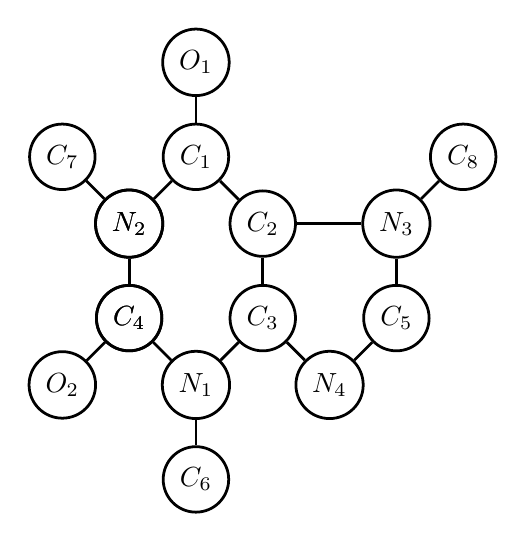
\begin{tikzpicture}[node distance={12mm}, line width=1pt, main/.style = {draw, circle}] 
\node[main] (1) []{$C_1$}; 
\node[main] (2) [below right of=1]{$C_2$}; 
\node[main] (3) [below of=2]{$C_3$}; 
\node[main] (4) [below left of=3]{$N_1$}; 
\node[main] (5) [above left of=4]{$C_4$}; 
\node[main] (6) [above of=5]{$N_2$};
\node[main] (9) [below right of=3]{$N_4$}; 
\node[main] (8) [above right of=9]{$C_5$}; 
\node[main] (7) [above of=8]{$N_3$}; 
\node[main] (10) [above of=1]{$O_1$}; 
\node[main] (11) [above left of=4]{$C_4$}; 
\node[main] (12) [above of=5]{$N_2$}; 

\node[main] (13) [below of=4]{$C_6$};  

\node[main] (17) [below left of=5]{$O_2$};

\node[main] (18) [above left of=6]{$C_7$}; 

\node[main] (22) [above right of=7]{$C_8$}; 



\draw [] (1) -- (2); 
\draw [] (2) -- (3); 
\draw [] (3) -- (4); 
\draw [] (4) -- (5); 
\draw [] (5) -- (6); 
\draw [] (6) -- (1); 
\draw [] (2) -- (7); 
\draw [] (7) -- (8); 
\draw [] (8) -- (9); 
\draw [] (9) -- (3); 
\draw [] (1) -- (10); 

\draw [] (4) -- (13); 

\draw [] (5) -- (17); 

\draw [] (6) -- (18); 

\draw [] (7) -- (22); 
\end{tikzpicture}
% \end{center}
}}
		\quad
		\subfloat[][A Path Decomposition]{\resizebox{0.16\textwidth}{!}{% !TEX root = ../main.tex
% \begin{center}
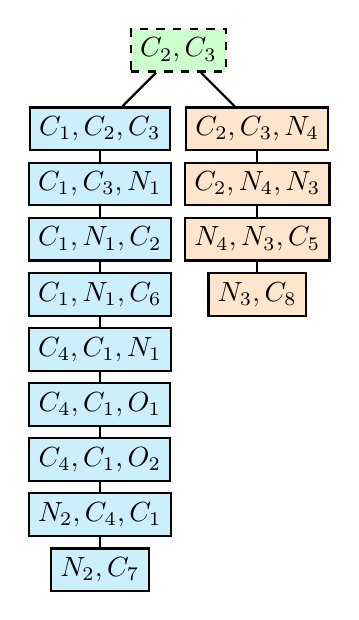
\begin{tikzpicture}[node distance={7mm}, thick, main/.style = {draw, rectangle}] 
\node[main, fill=green!20, dashed] at (0,0) (8) {$C_2,C_3$};
\node[main,fill=cyan!20] at (-1,-1) (7){$C_1,C_2,C_3$};
\node[main,fill=cyan!20] (100) [below of =7] {$C_1,C_3,N_1$};
\node[main,fill=cyan!20] (6) [below of =100]{$C_1,N_1,C_2$};
\node[main,fill=cyan!20] (5) [below of =6]{$C_1,N_1,C_6$};
\node[main,fill=cyan!20] (4) [below of =5]{$C_4,C_1,N_1$};
\node[main,fill=cyan!20] (3) [below of =4]{$C_4,C_1,O_1$};
\node[main,fill=cyan!20] (2) [below of =3]{$C_4,C_1,O_2$};
\node[main,fill=cyan!20] (1) [below of =2]{$N_2,C_4,C_1$};
\node[main,fill=cyan!20] (0) [below of =1] {$N_2,C_7$}; 

%\node[main,white] (00) [right = 1cm of 0] {}; 
%\node[main,white] (000) [left = 1cm of 0] {}; 



\node[main,fill=orange!20] at (1, -1) (9){$C_2,C_3,N_4$};
\node[main,fill=orange!20] (10) [below of =9]{$C_2,N_4,N_3$};
\node[main,fill=orange!20] (11) [below of =10]{$N_4,N_3,C_5$};
\node[main,fill=orange!20] (12) [below of =11]{$N_3, C_8$};


\draw [] (0) -- (1); 
\draw [] (1) -- (2); 
\draw [] (2) -- (3); 
\draw [] (3) -- (4); 
\draw [] (4) -- (5); 
\draw [] (5) -- (6); 
\draw [] (6) -- (100); 
\draw [] (7) -- (100); 
\draw [] (7) -- (8); 
\draw [] (8) -- (9); 
\draw [] (9) -- (10); 
\draw [] (10) -- (11); 
\draw [] (11) -- (12); 


\end{tikzpicture}
% \end{center}}}
		\quad
		\subfloat[][A Tree Decomposition]{\resizebox{0.3\textwidth}{!}{% \begin{center}
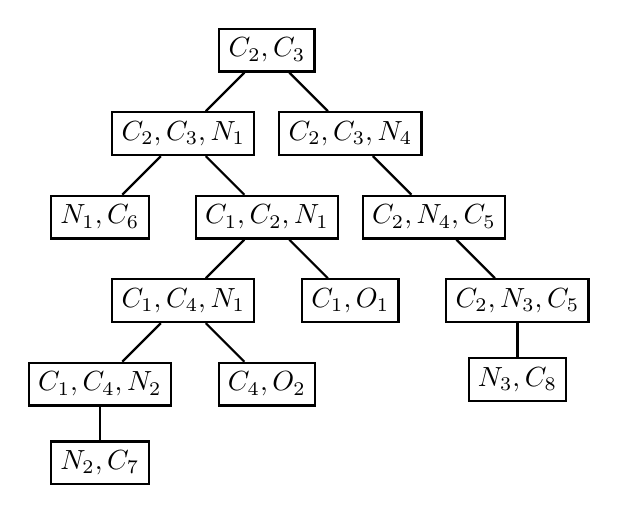
\begin{tikzpicture}[node distance={15mm}, thick, main/.style = {draw, rectangle}] 
\node[main] (0) []{$C_2,C_3$}; 
\node[main] (00) [below left of =0]{$C_2,C_3,N_1$};
\node[main] (000) [below left of =00]{$N_1,C_6$};
\node[main] (001) [below right of =00]{$C_1,C_2,N_1$};
\node[main] (0011) [below right of =001]{$C_1,O_1$};
\node[main] (0010) [below left of =001]{$C_1,C_4,N_1$};
\node[main] (00101) [below right of =0010]{$C_4,O_2$};
\node[main] (00100) [below left of =0010]{$C_1,C_4,N_2$};
\node[main] (001000) [below of =00100,,node distance={10mm}]{$N_2,C_7$};
\node[main] (01) [below right of =0]{$C_2,C_3,N_4$};
\node[main] (011) [below right of =01]{$C_2,N_4,C_5$};
\node[main] (0111) [below right of =011]{$C_2,N_3,C_5$};
\node[main] (01110) [below of =0111,,node distance={10mm}]{$N_3,C_8$};

\draw [] (0) -- (00); 
\draw [] (00) -- (000); 
\draw [] (00) -- (001); 
\draw [] (001) -- (0010); 
\draw [] (001) -- (0011); 
\draw [] (0010) -- (00100); 
\draw [] (00100) -- (001000);  
\draw [] (0010) -- (00101); 

\draw [] (0) -- (01); 
\draw [] (01) -- (011); 
\draw [] (011) -- (0111); 
\draw [] (0111) -- (01110); 

\end{tikzpicture}
% \end{center}}}
		\caption{A Graph Representation of Caffeine and a path and tree decomposition of this graph. Vertices in the root bag of the tree decomposition are highlighted in green (dashed). Notice how the removal of these nodes in the original molecule separates it into two connected components, each corresponding to one of the sides of the path decomposition, and one of the highlighted subtrees in the tree decomposition.}
		\label{fig:tree_dec_caffeine}
	\end{figure}

\end{example}
% \begin{figure}[H]
% 	\centerin{}g
% 	\chemfig{=^[:270](-[:330]=^[:30]-[:90]=^[:150]-[:210])-[:210]=_[:270](%
-[:330]=_[:30]-[:330]=_[:270]-[:210]=_[:150]-[:90])-[:210](-[:270]=_[:330]%
-[:270]=_[:210]-[:150]=_[:90]-[:30])=_[:150](-[:210]=_[:270]-[:210]=_[:150]%
-[:90]=_[:30]-[:330])-[:90](-[:150]=^[:90]-[:150]=^[:210]-[:270]=^[:330]%
-[:30])=_[:30](-[:330])-[:90]=^[:30]-[:90]=^[:150]-[:210]=^[:270](-[:330])}

% 	\caption{1,2,3,4,5,6-hexakis-phenylbenzene}
% 	\label{fig:tw_2 example}
% \end{figure}

\begin{lemma}[Proof in~\ref{app:proof}]\label{intseplemma}
	If $b$ is an introduce node with a single child $c$ and $X_b = X_c \cup \{v\}$, then $N(v)\cap G_b^\downarrow \subseteq X_c$. Here, $N(v)$ is the set of neighbors of $v.$
\end{lemma}



\begin{lemma}[Proof in~\ref{app:proof}]\label{joinseplemma}
	If $b$ is a join node with two children $c_1$ and $c_2,$ then in $G_b^\downarrow$ there is no edge with one endpoint in $V(G_{c_1}^\downarrow) \setminus X_b$ and the other in $V(G_{c_2}^\downarrow) \setminus X_b.$ Informally, $X_b$ is a cut that separates $V(G_{c_1}^\downarrow)$ from $V(G_{c_2}^\downarrow)$ in $G.$ See Figure~\ref{fig:tree_dec_caffeine}.
\end{lemma}

% \begin{proof}
% Let $T^\prime, T^{\prime\prime}, T^{\prime\prime\prime}$ be the subtrees of $T$ rooted at $b, c_1, c_2$ respectively. Let 
% $\mathcal{T}^\prime, \mathcal{T}^{\prime\prime}, \mathcal{T}^{\prime\prime\prime}$ be the corresponding tree decompositions. We will prove the given statement by contradiction. Therefore, let us assume that $u \in V(G_{c_1}^\downarrow) \setminus X_b$, $v \in V(G_{c_2}^\downarrow) \setminus X_b$, and $uv \in E(G_b^\downarrow)$.

% As $\mathcal{T}^{\prime}$ is a tree decomposition of $G^\downarrow_b$, there exists at least one bag $X_t$, such that $t \in \mathcal{T}^{\prime}$ and $u,v \in X_t$. From our initial assumption, we know that $u, v \notin X_b$, this implies that $t \neq b$. Therefore, either $t \in T^{\prime\prime}$ or $t \in T^{\prime\prime\prime}$. Without loss of generality, let us assume that $t \in T^{\prime\prime}$. As $v \in V(G_{c_2}^\downarrow) \setminus X_b$, there exists at least one bag $X_s$ such that, $ s \in T^{\prime\prime\prime}$ and $v \in X_s$. Observe that $v$ appears in both bags $X_s$ and $X_t$. Now by Definition \ref{def:tree_dec}, we know that $T^\prime_{v}$ is a connected subtree and any path connecting $s$ and $t$ goes through $b$. This implies that $X_b \in T^\prime_v$ and $v \in X_b$. This contradicts our initial assumption that $v \notin X_b$, hence completes the proof.
% \end{proof}

\section{Problem Statement}
\label{sec:p_statement}
\paragraph{Omega-regular Objectives.}
An $\omega$-regular objective is defined by a nondeterministic B\"uchi automaton $\oautomata = (\alphabets, \ostate, \oinitstate, \otrans, F)$ where $\alphabets$ is a finite \emph{alphabet}, $\ostate$ is a finite set of \emph{states}, $\oinitstate \in \ostate$ is an \emph{initial state}, $\otrans : \ostate \times \alphabets \rightarrow 2^\ostate$ is a \emph{transition function} and $F \subseteq \ostate$ is the set of \emph{accepting states}.
A B\"uchi automaton is deterministic, if $\delta(q, a)$ is singleton for all $(q, a) \in \ostate{\times}\alphabets$.
We define the extended transition function $\hat{\otrans}: \ostate \times \alphabets^* \rightarrow 2^\ostate$, derived from $\otrans$, as 
% \[
% \hat{\otrans}(q, w) = \begin{cases}
% \set{q} & \text{ if $ w = \varepsilon$}\\
% \bigcup\limits_{q' \in \otrans(q, a)} \hat{\otrans}(q', x) & \text{ if } w = ax \text{ for } a {\in} \Sigma, x {\in} \Sigma^*.
% \end{cases}
% \]
 $\hat{\otrans}(q, \varepsilon) = \set{q}$ and $\hat{\otrans}(q, ax) = \cup_{q' \in \otrans(q, a)} \hat{\otrans}(q', x)$, for $q \in \ostate$ and $ax \in \Sigma\Sigma^*$.

% B{\"u}chi automaton by \textbf{DBW}.

A \emph{run} $r$ of $\oautomata$ is an infinite sequence $(r_0, w_0, r_1, w_1, \ldots)$ where $r_0 = q_0$, $r_i \in \ostate$, $w_i \in \alphabets$ and $r_{i+1} \in \otrans(r_i,w_i)$ for all $i \in \mathbb{N}$. The word of a run $r = (r_0, w_0, r_1, w_1, \ldots)$ is ${\sf L}(r)=(w_0 w_1 \cdots)$ . Let the set of runs of $\oautomata$ be $\oruns$.
We say that a run $r \in \oruns$ is accepting if there exists a $q_f \in F$ such that $q_f$ occurs infinitely often in $r$. An $\omega$-word $w = (w_0 w_1 \cdots)$ is accepted by $\oautomata$ if there exists an accepting run $r_w = (r_0, w_0, r_1, w_1, \ldots)$ of $\oautomata$. 
The language of the automaton $\oautomata$, denoted $\Ll(\oautomata)$ is the set of all words that is accepted by the automaton. 

\paragraph{CTMDPs and Omega-regular Objectives.}
In order to express the properties of a CTMDP $\Mdp$ using a B\"uchi automaton, we introduce the notion of a labelled CTMDP.
A \emph{labelled} CTMDP is a triple $(\Mdp, \atomicprop, \labelling)$ where $\Mdp$ is a CTMDP, $\atomicprop$ is a set of atomic propositions, and $\labelling: \states \rightarrow 2^\atomicprop$ is a labelling function. 
Let $\oautomata = (2^{\atomicprop}, \ostate, \oinitstate, \otrans, \acceptingc)$ be a B\"uchi automaton expressing the learning objectives of $\Mdp$.

Recall that for a CTMDP $\Mdp$ under a schedule $\sigma$ we write $X_n$, $Y_n$, $D_n$, and $T_n$ for the random variables corresponding to the $n$-th state, action, time-delay at the $n$-th state, and time-stamp (total time spent up to the $n$-th state).
We introduce the random variable $F_n$ to indicate if the sequence of observations of the CTMDP leads to an accepting state on $\oautomata$ in $n$-steps, i.e., 
$
F_n = [\hat{\delta}(L(X_0)\cdot L(X_1) \cdots L(X_n)) \cap F].
$

For a CTMDP $(\Mdp, \atomicprop, \labelling)$ and  automaton $\oautomata = (2^{\atomicprop}, \ostate, \oinitstate, \otrans, \acceptingc)$,
we study the following problems:
\begin{enumerate}
    \item {\bf Satisfaction Semantics.} 
    Compute a schedule of $\Mdp$ that maximizes the probability of visiting accepting states $F$ of $\oautomata$ infinitely often.
    We define the satisfaction probability of a schedule $\sigma$ from starting state $s$ as: 
\begin{equation*}
\PSemSat^{\Mdp}_{\oautomata}(s, \sigma) 
{=}   {\Pr}^{\Mdp}_{\sigma}(s) \set{\forall_i  \exists_{j{\geq} i} F_j }.
\end{equation*}
% \begin{equation*}
% \PSemSat^{\Mdp}_{\oautomata}(s, \sigma) 
% {=}   \Pr{}^{\Mdp}_{\sigma}(s) \set{ r \in \Runs_{\sigma}^{\Mdp}(s) \colon
%   L(r) \in \Ll(\oautomata) }.
% \end{equation*}
% i.e, the probability of runs from $s$ under $\sigma$ for which its corresponding run in $\oautomata$ visits an accepting state infinitely often.
Intuitively, it describes the probability of runs from state $s$ under $\sigma$ in the CTMDP such that the corresponding run in $\oautomata$ visits the accepting states infinitely often.
The optimal satisfaction probability
$\PSemSat^{\Mdp}_{\oautomata}(s)$ for  $\oautomata$ 
is defined as $\sup_{\sigma \in \Sigma_{\Mdp}} \PSemSat^{\Mdp}_{\oautomata}(s, \sigma)$, and we say
that a schedule $\sigma \in \Sigma_\Mdp$ is an optimal schedule for $\oautomata$ if
$\PSemSat^{\Mdp}_{\oautomata}(s, \sigma)  = \PSemSat^{\Mdp}_{\oautomata}(s)$ for all $s \in \states$.

\item {\bf Expectation Semantics.} Compute a schedule of $\Mdp$ that maximizes the long-run expected average time spent in the accepting states of $\oautomata$.
We define the expected satisfaction time of a schedule $\sigma$ from starting state $s$ as: 
\begin{equation*}
\ESemSat{}^{\Mdp}_{\oautomata}(s, \sigma) 
=   \mathbb{E}^{\Mdp}_{\sigma}(s) \set{ \liminf_{n \rightarrow \infty} \frac{\sum_{i=1}^{n} F_i \cdot D_i}{T_n}}.
\end{equation*}
The optimal expected satisfaction time
$\ESemSat^{\Mdp}_{\oautomata}(s)$ for specification $\oautomata$ is defined as $\sup_{\sigma \in \Sigma_{\Mdp}} \ESemSat^{\Mdp}_{\oautomata}(s, \sigma)$, and we say that $\sigma \in \Sigma_\Mdp$ is an optimal expectation maximisation schedule for $\oautomata$ if $\ESemSat^{\Mdp}_{\oautomata}(s, \sigma) = \ESemSat^{\Mdp}_{\oautomata} (s)$.
\end{enumerate}


\paragraph{Product Construction.} 
Given a \emph{labelled} CTMDP $(\Mdp, \atomicprop, \labelling)$ where $\atomicprop$ is a set of atomic propositions, and $\labelling: \states \rightarrow 2^\atomicprop$ is a labelling function, and a   B{\"u}chi automaton $\oautomata = (2^{\atomicprop}, \ostate, \oinitstate, \otrans, \acceptingc)$, the product CTMDP is defined as $\Mdp \times \oautomata = ((\states \times \ostate),(\initstate,\oinitstate),\actions,\transR^{\times},\acceptingc^{\times})$ where the rates are $\transR^{\times} : (\states \times \ostate) \times \actions \times (\states \times \ostate) \rightarrow \Reals_{\geq 0}$ such that $\transR^{\times} ((s,q),a,(s',q')) = \transR(s,a,s')$ if $\transR(s,a,s')>0$ and $\otrans (q,\labelling(s)) = \{q'\}$.
If $F$ is the set of accepting 
% transitions 
states
in $\oautomata$, then the accepting condition is a set 
% transitions $F^\times$ where $((s,q),a,(s',q')) \in F^\times$ iff $(q,\labelling(s),q') \in F$ 
$F^\times$ of states where $(s,q) \in F^\times$ iff $q \in F$. 
 An example of a product CTMDP is given in Appendix~\ref{sat vs expt}.  



\paragraph{Good-for-CTMDP Automata.} 
From the definition of both the semantics, it is clear that the optimal schedule requires some memory to monitor the run in the B\"uchi automaton (see Example~\ref{ex:mem} in Appendix~\ref{exmp:memory}).
% It is easy to see that for both optimization problems, the optimal schedules require memory.
For the right kind of B\"uchi automata~\cite{HPSS20}, the amount of memory required can be equal to the size of the automata. 
A key construction to compute these schedules is the product construction, where the CTMDP and the automaton are combined together as a CTMDP with accepting states governed by the accepting states of the B\"uchi automata.
On the other hand, not every B\"uchi automaton can be used for this construction.
The class of B\"uchi automata where the semantic value of satisfaction of the property on the MDP equals to the corresponding problems on the product structure, are called good-for-MDP (GFM) automata~\cite{HPSS20}.

We introduce the notion of good-for-CTMDP automata in Appendix~\ref{app:gfm}.
% We also argue that every $\omega$-regular property can be expressed as a good-for-CTMDP automaton\todo{add a reference}. 
If a B\"uchi automaton is GFM, then one can show via uniformization that it is also good-for-CTMDPs.
There exist several syntactic characterizations of good-for-MDP automata including suitable limit-deterministic B\"uchi automata (SLDBA)~\cite{sickert2016limit} and slim automata~\cite{HPSS20}.
Moreover, every LTL specification can be effectively converted into a GFM B\"uchi automata.
Moreover, there exist tools (OWL and Spot) to convert LTL objectives to good-for-CTMDP automaton.
Hence, in this paper, w.l.o.g., we assume that $\omega$-regular objectives are given as good-for-CTMDP automata.


% Let for a run $r$, we denote by $\inf(r)$ the set of states visited infinitely often in $r$.
% A run $r$ of $\Mdp \times \mathcal{A}$ is accepting if
% $\inf(r) \cap F^\times \neq \emptyset$.
% We define the
% \emph{syntactic satisfaction}
% probabilities $\PSat^\Mdp_{\oautomata}((s,q), \sigma^\times)$ as the probability of
% accepting runs, i.e.
% \[
% \Pr{}^{\Mdp\times\oautomata}_{\sigma^\times}(s,q) \Set{ r \in
% \Runs_{\sigma^\times}^{\Mdp\times\oautomata}(s,q) : \inf(r) \cap F^\times
% \neq \emptyset }
% \]
% Similarly, we define $\PSat^\Mdp_{\oautomata}(s)$ as the optimal probability over the
% product, i.e.  $\sup_{\sigma^\times}\big(\PSat^\Mdp_{\oautomata}((s,q_0),
% \sigma^\times)\big)$.
% For a deterministic $\oautomata$ the equality $\PSat^\Mdp_{\oautomata}(s) = \PSemSat^\Mdp_{\oautomata}(s)$ holds; however it is not guaranteed for nondeterministic
% B\"uchi automata as the optimal resolution of nondeterministic
% choices may require access to future events.
% However, while \textbf{DBW}s cannot capture all of $\omega$-regular properties, it has been shown in \cite{HahnPSSTW19} that specifying an $\omega$-regular objective with a deterministic Rabin automaton is not always suitable for defining a reward mechanism necessary for reinforcement learning.
% This motivates for the definition of a good-for-MDP nondeterminisitc B\"uchi automata.
% A B\"uchi automaton $\oautomata$ is \emph{good for MDPs} (GFM),
% if $\PSat^\Mdp_{\oautomata}(s_0) = \PSemSat^\Mdp_{\oautomata}(s_0)$ holds for all
% MDPs $\Mdp$ and starting states $s_0$ \cite{Hahn20}.
% Note that every $\omega$-regular objective can be expressed as a GFM automaton \cite{Hahn20}.

% \track{CHECK IF ACCEPTING END-COMPONENT DEFINED LATER.}
\begin{comment}
For a product CTMDP, we define run and end-component in the same way as that of a CTMDP. An accepting run is a run which visits an accepting 
% transition 
state
infinitely often. An end-component is accepting if it has an accepting state.
% transition. 
    
{\color{red} After introducing nondeterminsitic B\"uchi, a quick paragraph about why nondeterminism is required, why we need to have LDBWs? Just make an assumption that all Buchi considered are LDBWs. We can do so without definition, and move the definition to the appendix, if allowed.}
\paragraph{Limit Deterministic B{\"u}chi Automaton.}
A nondeterministic B{\"u}chi automaton accepting $\omega$-words (\textbf{NBW}) can represent all $\omega$-regular objectives, while a \textbf{DBW} cannot. We define another B{\"u}chi automaton which adds some non-determinism to \textbf{DBW}s and have the same expressiveness as \textbf{NBW}. This automata is called a \emph{limit deterministic} B{\"u}chi automata (\textbf{LDBW}). Intuitively, an \textbf{LDBW} consists of a non-deterministic component without accepting states, and a deterministic component with only accepting states. The automaton can only accept by moving from the non-deterministic component to the deterministic component, and once it reaches the deterministic component, it stays there forever. 
Formally, an \textbf{LDBW} is an \textbf{NBW} $\oautomata = (\alphabets,\ostate_{N} \cup \ostate_{D},\oinitstate,\otrans,F)$ where 
\begin{inparaenum}[(1)]
    \item $\ostate_{N} \cap \ostate_{D} = \emptyset$, $F \subseteq \ostate_{D}$;
    \item $|\otrans(q,\sigma)| \leq 1$ for all $q \in \ostate_{D}$ and $\sigma \in \alphabets$;
    \item $\otrans(q,\sigma) \subseteq \ostate_{D}$ for all $q \in \ostate_{D}$ and $\sigma \in \alphabets$.
\end{inparaenum}
% \track{Definition of suitable LDBW?}\\
A suitable limit deterministic B{\"u}chi automata (\textbf{GFM}) $A$ for a property $\phi$ is an \textbf{LDBW} that recognises $\phi$ and such that, for any finite MDP $\Mdp$, there exists a pure schedule $\sigma$ such that the probability of satisfying the B{\"u}chi condition in $(\Mdp \times A)_{\sigma}$ is the same as the probability of satisfying $\phi$ in $\Mdp$ by an optimal schedule in $\Mdp$.
We can similarly define \textbf{GFM} for a CTMDP $\Mdp$.

Not every \textbf{LDBW} is suitable. Consider the  pair of automata shown in Figure~ \ref{fig:P2} for $(\always a)\lor(\always b)$. The automaton in right is suitable as the initial state $q_0$ can delay the transition to state $q_1$ or $q_2$ by staying in $q_0$, and move only when the end-component of the CTMDP is reached. The automaton in the left is not suitable as we have to pick the transition to state $q_1$ or $q_2$ immediately and cannot wait until an end-component is reached. But as we can see, both the automata accept the same language. 
\begin{theorem}[\cite{courcoubetis1995complexity},\cite{hahn2013lazy},\cite{sickert2016limit},\cite{vardi1985automatic}]\label{GFM}
Suitable limit deterministic B{\"u}chi automata exist for all $\omega$-regular languages. 
\end{theorem}
\begin{figure}[t]
    \centering
    \begin{subfigure}[b]{0.4\linewidth}
    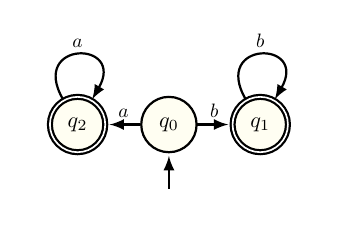
\begin{tikzpicture}[shorten >=1pt, node distance=3 cm, on grid, auto,thick,initial text=,]
\begin{scope}[every node/.style={scale=.8}]
\node (l0) [state,initial below, fill = safecellcolor] {$q_0$};
\node (l1) [state,right = of l0,xshift = -2.3cm,accepting, fill = safecellcolor]   {$q_1$};
\node (l2) [state,left = of l0,xshift = 2.3cm,accepting,fill = safecellcolor]   {$q_2$};
\end{scope}
 \begin{scope}[every node/.style={scale=.7}]
\path [->]
    (l0) edge  node [above] {$b$}   (l1)
    (l0) edge  node [above] {$a$}   (l2)
    (l1) edge [loop above] node [above] {$b$}   ()
    (l2) edge [loop above] node [above] {$a$}   ()
    ;
\end{scope}
\end{tikzpicture}
    \label{fig:P2.1}
    \end{subfigure}
\begin{subfigure}[b]{0.4\linewidth}
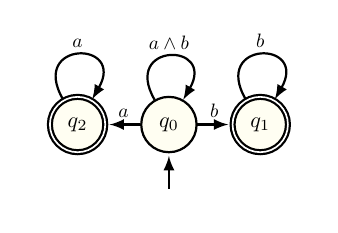
\begin{tikzpicture}[shorten >=1pt, node distance=3 cm, on grid, auto,thick,initial text=,]
\begin{scope}[every node/.style={scale=.8}]
\node (l1) [state,accepting,fill = safecellcolor]   {$q_1$};
\node (l0) [state,initial below,left = of l1,xshift = 2.3cm,fill = safecellcolor] {$q_0$};

\node (l2) [state,left = of l0,xshift = 2.3cm,accepting, fill = safecellcolor]   {$q_2$};
\end{scope}
 \begin{scope}[every node/.style={scale=.7}]
\path [->]
    (l0) edge [loop above]  node {$a \land b$}()
    (l0) edge  node [above] {$b$}   (l1)
    (l0) edge  node [above] {$a$}   (l2)
    (l1) edge [loop above] node [above] {$b$}   ()
    (l2) edge [loop above] node [above] {$a$}   ()
    ;
\end{scope}
\end{tikzpicture}
\label{fig:P2.2}
\end{subfigure}
    
    \caption{Unsuitable(left) and suitable(right) \textbf{LDBW} for the LTL formula $(\always a) \lor (\always b)$ from  \cite{hahn2013lazy}}
    \label{fig:P2}
\end{figure}
\end{comment}



% Our objective is to get an optimal schedule $\sigma$ for a given $\omega$-regular objective $\phi$ and a CTMDP $\Mdp$ with unknown transition structure using model-free learning algorithms. Model-free learning algorithms can be used only if we can define rewards that depend on the observations from the CTMDP and the satisfaction of the property. We use a product CTMDP $\pmdp$ where $\Mdp$ is a CTMDP and $\oautomata$ is an \textbf{GFM}. A product CTMDP can be used to monitor both the observations from the CTMDP and the satisfaction of the given property. Using \textbf{GFM} has been shown to give an optimal schedule in MDPs \cite{HahnPSSTW19}. We give a formal proof that we can use a similar approach on CTMDPs and get an optimal schedule. 

% \track{Are we going to consider the objective of maximizing dwell time, i.e. find a schedule for maximizing the expected dwell time. In that case, what is the use of $\omega$-regular objective? This is simply an average optimization problem. I don't see the need for LDBA any more, or a product construction as this is no longer a qualitative but a quantitative objective.}

% We note here that while composing with an MDP, it is preferred that the specification is given in terms of a deterministic automaton \cite{vardi1985automatic}.

% \vspace{0.5em}\noindent\textbf{Two Semantics.} We consider two semantics for satisfaction of $\phi$ in the context of a CTMDP in which a run includes passage of real time.
% In the first one of the two semantics, the objective is to maximise the residence time in the ``good states'' which are the set of accepting states of the \textbf{GFM}. To apply model-free RL algorithms, we need to define suitable reward mechanisms based on the observations made on the CTMDP environment.
% The reward mechanisms should be designed in a way to capture the specific objective in a model with continuous time semantics. It may be desirable to satisfy the property with certain quality, which is reflected using maximising the residence time in those states. We also refer to this semantics as the \emph{expectation semantics}.
% For an infinite run $r_{inf}=(s_1,t_1,a_1,s_2,t_2,a_2, \ldots)$ of a given CTMDP $\Mdp$ under schedule $\sigma$, we define the residence time of $s$ in $r_{inf}$ as 
% \[
% Rt^{\Mdp^{\sigma}}(s)(r_{inf}) = \liminf_{n \rightarrow \infty} \frac{\sum_{i=1}^{n} [s_i = s] \cdot t_i}{\sum_{j=1}^{n}t_j}.
% \]
% % Note that we consider $\liminf$ since the limit may not exist in general.
% For a set $T$ of good states and the infinite run $r_{inf}$, we define residence time of $T$ under schedule $\sigma$ as 
% % \todo{Should we use equation environment}
% \[
% Rt^{\Mdp^{\sigma}}(T)(r_{inf}) = \liminf_{n \rightarrow \infty} \frac{\sum_{i=1}^{n} [s_i \in T] \cdot t_i}{\sum_{j=1}^{n}t_j}.
% \]
% In the expectation semantics, our goal is to find a schedule $\sigma^*$ that maximizes the expected residence time in the set $T$ of states, i.e.
% \[
% \mathbb{E} [Rt^{\Mdp^{\sigma^*}}(T)] = \sup_{\sigma \in \Sigma_\Mdp} \mathbb{E} [Rt^{\Mdp^{\sigma}}(T)].
% \]


% In the second semantics, we consider the satisfaction of $\omega$-regular objectives in the traditional sense, where an optimal schedule is one which maximises the probability of satisfying the $\omega$-regular objective.
% The frequency of visiting the ``good" states is not relevant for the satisfaction of the objective.
% We refer to this semantics as the \emph{satisfaction} semantics.
% In the satisfaction semantics, given a CTMDP $\Mdp$, and an $\omega$-regular objective $\phi$, our goal is to find a schedule $\sigma^*$ such that \track{WHY $\geq$ BELOW?}
% \[
% \Pr[\Mdp^{\sigma^*} \models \phi] \geq \sup_{\sigma \in \Sigma_\Mdp} \Pr[\Mdp^{\sigma} \models \phi],
% \]
% where $\Pr[\Mdp^{\sigma} \models \phi]$ denotes the probability of satisfying $\phi$ by the CTMDP $\Mdp$ under schedule $\sigma$.

% We show in the following sections that we need different reward mechanisms for the two semantics in order to learn the corresponding optimal schedules using RL.

% \subsection{Reward Machines}
% Often, complex learning objectives cannot be expressed using Markovian reward
% signals. 
% A recent trend is to express learning objectives using finite-state reward
% machines~\cite{icarte2018using}. 
% We require a more expressive variant of reward machine capable of $\epsilon$ transitions\track{ARE WE USING $\epsilon$ TRANSITIONS? SIMPLER PRODUCT DEFINITION WITHOUT $\epsilon$.} and nondeterminism. We
% call them nondeterministic reward machines. 
% A (nondeterministic) reward machine is a tuple $\Rr = (\Sigma_\epsilon, U, u_0, \delta_r, \rho)$
% where $U$ is a finite set of states, $u_0 \in U$ is the starting state,
% $\delta_r: U \times \Sigma_\epsilon \to 2^U$ is the transition relation, 
% and $\rho: U \times \Sigma_\epsilon \times U \to \Reals$ is the reward function, where $\Sigma_\epsilon = (\Sigma\cup \set{\epsilon})$ and $\epsilon$ is a special silent transition.

% Given a labelled MDP $\Mdp = (S, s_0, A, T, AP, L)$\track{WE USE $\actions$ ELSEWHERE.} and a reward machine $\Rr = (\Sigma_\epsilon, U, u_0, \delta_r, \rho)$ over the alphabet $\Sigma = 2^{AP}$,  their product 
% $\Mdp\times\Rr = (S{\times} U, s_0 {\times} u_0, (A {\times} U) \cup\set{\epsilon},
% T^\times, \rho^\times)$
% is a rewardful MDP where
% $T^\times: (S {\times} U) \times ((A {\times} U) \cup \set{\epsilon}) \to \Distributions(S{\times} U)$ is such that
% $T^\times((s,u), \alpha)(({s}',{u}'))$ equals 
% \begin{multline*}
% %T^\times((s,u), \alpha)(({s}',{u}')) =\\
% \begin{cases}
% T(s,a)({s}') & \text{if } \alpha = (a, u') \text{ and } (u,L(s),u') \in \delta_r \\
% 1 & \text{if } \alpha = \epsilon \text{ and } s = s' \text{ and } \delta(u, \epsilon, {u}') \in \delta_r \\
% 0 & \text{otherwise.}
% \end{cases}
% \end{multline*}
% and $\rho^\times: (S{\times} U) \times ((A {\times}
% U) \cup \set{\epsilon}) \times (S{\times} U)\to \Reals$ is defined such that 
% $\rho^\times((s,u), \alpha, (s', u'))$ equals
% \begin{multline*}
% % \rho^\times((s,u), \alpha, (s', u')) =\\
% \begin{cases}
% \rho(u, L(s), u') & \text{if } \alpha = (a, u') \text{ and } (u,L(s),{u}') \in \delta_r \\
% \rho(u, \epsilon, u') & \text{if } \alpha = \epsilon.
% \end{cases}
% \end{multline*}
% For technical convenience, we assume that $\Mdp{\times}\Rr$ contains only reachable states from $(s_0, u_0)$.
% For both discounted and average objectives, the optimal strategies of
% $\Mdp{\times}\Rr$ are positional on $\Mdp{\times}\Rr$.
% Moreover, these positional strategies characterize a finite memory strategy (with memory skeleton based on the  states of $\Rr$ and the next-action function based on the positional strategy) over $\Mdp$
% maximizing the learning objective given by $\Rr$. 


\paragraph{Problem Definition.} Given a CTMDP $\Mdp$ with unknown transition structure and rates, and an $\omega$-regular objective $\phi$ given as a good-for-CTMDP B\"uchi automata $\oautomata$, we are interested in the following reward translation problem for the satisfaction semantics and for the expectation semantics. 

\begin{problem}[Reward Translation Scheme]
    Design a reward scheme for $\oautomata$ 
    % for satisfaction (expectation) semantics 
    such that any off-the-shelf RL algorithm optimizing the discounted reward in CTMDPs converges to an optimal schedule for satisfaction (expectation) semantics.
\end{problem}

In Section~\ref{sec:theorems&algo} we provide a solution for the satisfaction semantics, while in Section~\ref{sec:d_time} we sketch a solution for this problem for the expectation semantics.
% In both of these results, 
We reduce these problems to average reward maximization for CTMDPs.
Since average-reward RL algorithms for CTMDPs and MDPs require strong assumptions on the structure (such as communicating MDPs)~\cite{Sutton18}, we solve the average-reward RL problem by reducing it to a discounted-reward problem using the following result.
\begin{theorem}\label{corollary:1}
For every CTMDP $\Mdp$, there exists a pure schedule $\bschedule$ and a threshold $0 {\leq} \ctmdpthrate^{\Mdp} {<} 1$ such that
% \begin{inparaenum}[(1).]
    % \item 
    for every discount-rate function $\ctmdprate$, where $\ctmdprate(s,a) \geq \ctmdpthrate^{\Mdp}$ for every valid state-action pair $(s,a)$, the schedule $\bschedule$ is an optimal schedule maximising the expected discounted reward.
    % \item 
    Moreover, $\bschedule$ also maximizes the expected average reward.
% \end{inparaenum}
\end{theorem}
This schedule $\bschedule$ is known as a Blackwell optimal schedule.
We provide a novel uniformization based proof for this theorem in Appendix~\ref{sec:blackwell_optimality}.
We show that we need different reward translation schemes for the two semantics.

% In the next section, we provide a simple uniformization based proof for the Blackwell optimality for CTMDPs.
% \track{Add Theorem 3 here?}


\section{RL for Satisfaction Semantics}
\label{sec:theorems&algo}
% \vspace{0.5em}\noindent\textbf{Sub-MDP and End-Components.} For a given MDP $\Mdp= (S, s_0,\actions, T)$, a {\it sub-MDP} of $\Mdp$ is an MDP $\Mdp' = (S', s_0',\actions', T')$, where $S' \subset
% S$, $\actions' \subseteq \actions$ is such that $\actions'(s) \subseteq \actions{}(s)$,
% % \track{{\sf Act} in prelims instead of $A$} for every $s \in S'$,  
% and $T'$ is analogous to $T$ when restricted to $S'$ and
% $A'$. Moreover $\Mdp'$ is closed under probabilistic transitions.
% An {\it end-component}~\cite{alma991027942769706011} of an MDP $\Mdp$ is a sub-MDP $\Mdp'$ such that for every pair of states $s, s' \in S'$, there is a 
% schedule that can reach $s'$ from $s$ with positive probability. 
% A maximal end-component is an end-component that is maximal under set-inclusion.
% An end-component is \emph{winning} if it contains an accepting state.
% Every state $s$ of an MDP $\Mdp$ belongs to at most one maximal end-component.
% We can define sub-CTMDP, and end components in a CTMDP, as in the case of MDPs.
% % Further, we can see that Theorem~\ref{thm:ec} 
% Following is a property of end-components in an MDP that also holds for CTMDPs. 

%  \begin{theorem}[End-Component Properties \cite{alma991027942769706011}]\label{thm:ec}
% Once an end-component $C$ of an MDP is entered, there is a schedule that visits every state-action pair in $C$ with probability 1 and stays in $C$ forever. Moreover, for every schedule the probability that a run ends up in an end-component is 1.  
% \end{theorem}

% \vspace{0.5em}\noindent\textbf{Augmented Product CTMDP.} 
We reduce the problem of satisfaction semantics of an $\omega$-regular objective in a CTMDP to an expected average reward objective.
Using Blackwell optimality result stated in Theorem~\ref{corollary:1}, we further reduce this to an expected discounted reward objective which allows us to use off-the-shelf RL for CTMDP for learning schedules for $\omega$-regular objectives.

To find a schedule satisfying an $\omega$-regular objective in a CTMDP, we need to identify the accepting end-components where an accepting end-component~\cite{alma991027942769706011} is a sub-MDP that is closed under probabilistic transitions and contains an accepting state.
It is well known~\cite{alma991027942769706011} that as an end-component $C$ of an MDP is entered, there is a schedule that visits every state-action pair in $C$ with probability 1 and stays in $C$ forever.
Hence, a schedule that maximizes the probability of satisfaction of a given $\omega$-regular objective maximizes the probability of reaching the accepting end-components.
In Appendix~\ref{app:EC}, we show an example of a CTMDP and its end-components.
Also the MDP in the top part of Figure~\ref{fig:p3}, is itself an accepting end-component since the state $q_0$ is accepting.

% To tackle this problem, 
We further reduce the problem to an average reward problem as described below and then specify a reward function such that the schedule maximising the expected average reward maximizes the probability of satisfying the objective.
% Note that a reachability objective does not require identifying the end-components.
\paragraph{Reduction to Average Reward.}
Before describing our RL algorithm for unknown CTMDP, we first describe the reduction when an input CTMDP is fully known to explain the intuition behind our algorithm.
Consider a CTMDP $\Mdp$, a \textbf{GFM} $\oautomata$, and let $\pmdp$ denote the product CTMDP.
For our reduction, we define a constant $\zeta \in (0,1)$ and an augmented product CTMDP, denoted by $\augmdp$. 
The CTMDP $\augmdp$ is constructed from $\pmdp$ by adding a new sink state $t$ with a self loop labelled by an action $a'$ and with rate $\lambda(t,a') > 0$, and making it the only accepting state in $\augmdp$. 
Further, in $\augmdp$, the rates of each outgoing transition from an accepting state in $\pmdp$ is multiplied by $\zeta$. 
Also, for each action $a$ from an accepting state $s$ in $\pmdp$, in $\augmdp$ we add a new transition to the sink state $t$ with rate $\lambda(s,a) \cdot (1-\zeta)$ where $\lambda(s,a)$ is the exit rate of the state-action pair $(s,a)$ in $\pmdp$. 
% We also add an action $a'$ from $t$ with a single transition to itself.
% The rate of this action can be any positive constant $\lambda(t,a')$.
% as there are no other transition from $t$ and if the system reaches $t$ it will stay there forever.    
Figure~\ref{fig:p3} shows an example of this construction.
% \track{WHAT IS $\lambda(t,a')$? NEEDS TO BE ADDED.}
Note that in the figure, $q_0$ is the only accepting state in the product CTMDP.
There are two outgoing transitions from $q_0$ on action $a$ to $q_1$ and $q_2$ with rates $r_1$ and $r_2$ respectively, and hence $\lambda(q_0, a) = r_1 + r_2$.
% We add a sink $t$ which is the only accepting state in $\Mdp^\zeta$.
We then add a transition from $q_0$ to $t$ with rate $(r_1+r_2) \cdot (1-\zeta)$.

\begin{figure}[t]
 \centering
  \begin{minipage}{0.3\textwidth}
     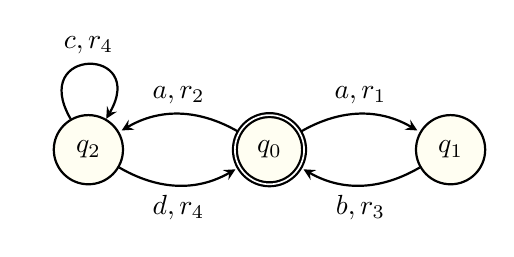
\begin{tikzpicture}[shorten >=1pt, node distance=2.3 cm, on grid, auto,thick,initial text=]
\begin{scope}[every node/.style={scale=1}]
\node (l0) [state,accepting, fill = safecellcolor] {$q_0$};
\node (l1) [state,right = of l0, fill = safecellcolor]   {$q_1$};
\node (l2) [state,left = of l0,fill = safecellcolor]   {$q_2$};
\end{scope}
 \begin{scope}
\path [-stealth, thick]
    (l0) edge [bend left]  node [above] {$a,r_1$}   (l1)
    (l0) edge [bend right]   node [above] {$a,r_2$}   (l2)
    (l1) edge [bend left]  node [below] {$b,r_3$}   (l0)
    (l2) edge  [loop above] node [above] {$c,r_4$}   ()
    (l2) edge [bend right] node [below] {$d, r_4$} (l0)
    ;
\end{scope}
\end{tikzpicture}
  \end{minipage}
  \begin{minipage}{0.3\textwidth}
    \centering
     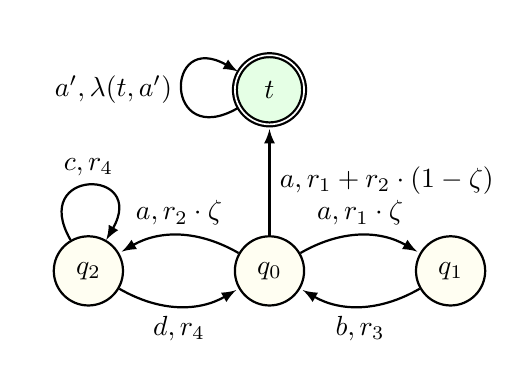
\begin{tikzpicture}[shorten >=1pt, node distance=2.3 cm, on grid, auto,thick,initial text=,]
\begin{scope}[every node/.style={scale=1}]
\node (l0) [state,fill = safecellcolor] {$q_0$};
\node (l1) [state,right = of l0, fill = safecellcolor]   {$q_1$};
\node (l2) [state,left = of l0,fill = safecellcolor]   {$q_2$};
\node (l3) [state, above = of l0,accepting, fill = goodcellcolor] {$t$};
\end{scope}
 \begin{scope}
\path [->]
    (l0) edge [bend left]  node [above] {$a,r_1  \cdot \zeta$}   (l1)
    (l0) edge  [bend right] node [above] {$a,r_2 \cdot \zeta$}   (l2)
    (l1) edge [bend left]  node [below] {$b,r_3$}   (l0)
    (l2) edge  [loop above] node [above] {$c,r_4$}   ()
    (l0) edge node [right] {$a,r_1+r_2 \cdot(1-\zeta)$}(l3)
    (l3) edge [loop left] node [left] {$a', \lambda(t,a')$} () 
    (l2) edge [bend right] node [below] {$d, r_4$} (l0)
    ;
\end{scope}
\end{tikzpicture}
  \end{minipage}
  \caption{A product CTMDP $(\Mdp \times \oautomata)$ (top) and its corresponding augmented product CTMDP $\Mdp^{\zeta}$ (bottom).}
  \label{fig:p3}
\end{figure}

% As we can see, the set of states in $\pmdp$ and $\augmdp$ differ only by $t$ and any run that reaches $t$ will stay there. 
% Therefore, given a schedule $\sigma$ in $\augmdp$, the corresponding schedule in $\pmdp$ is defined in a way where the action chosen from any state in $\pmdp$ will be the same as that of $\sigma$.
With a slight abuse of notation, if $\sigma$ is a schedule in the augmented CTMDP $\Mdp^\zeta$, then we also denote by $\sigma$ a schedule in $\Mdp \times \oautomata$ obtained by removing $t$ from the domain of $\sigma$.
Thus fix a schedule $\sigma$ in both $\Mdp^\zeta$ and in $\Mdp \times \oautomata$.
Note that for every state in an accepting end-component, the probability of reaching the sink $t$ in $\Mdp^\zeta$ is $1$.
Similarly, for every state in a rejecting end-component, the probability of reaching $t$ in $\Mdp^\zeta$ is $0$.
The probability of reaching $t$ in $\Mdp^\zeta$ under $\sigma$ overapproximates the probability of reaching the accepting end-components in $\Mdp \times \oautomata$ under $\sigma$.
The difference in the two probabilities occurs since in $\Mdp^\zeta$, from the transient accepting states, with probability $1-\zeta$, one can reach the sink $t$.
This approximation error tends to $0$ as $\zeta$ tends to $1$.
We define a reward function in $\augmdp$ such that a schedule maximising the expected average reward in $\augmdp$ maximizes the probability of satisfying the $\omega$ regular objective in $\pmdp$. 


% For a given CTMDP $\Mdp$, an embedded MDP $\embeddedMdp$ of $\mathcal{M}$ is a discrete-time MDP of the form $\embeddedMdp = (\states, \initstate, \actions{}, \transP_{\Mdp})$, that is, the transition function of $\embeddedMdp$ is derived from the probability matrix of $\Mdp$.
% As the set of states and enabled actions from each state are the same in $\Mdp$ and $\emdp$, the set of pure schedules in them are also same. 

% Time does not play a role in the definition of pure schedules. Therefore, the probability of reaching a state $s$ from the initial state in a CTMDP $\Mdp$ under a pure schedule $\sigma$ is dependant only on the transition function of the embedded MDP $\emdp$. 
% Now recall that for $\omega$-regular objectives, given a B\"{u}chi GFM, the states of the accepting condition of the product CTMDP need to be visited infinitely often.
% As there exist optimal pure schedules for reaching such states, we get the following lemma for an $\omega$-regular objective $\phi$.

% \begin{lemma} \label{lem:embedded}
% There exists a pure schedule that maximises the probability of satisfying $\phi$ in $\mathcal{M} \times \mathcal{A}$ which also maximises the probability of satisfying $\phi$ in the embedded product DTMDP $\mathcal{M}_\mathcal{E} \times \mathcal{A}$.
% \end{lemma}
% \begin{comment}
% Theorem 3 from \cite{HahnPSSTW19} gives us the existence of a threshold $\zeta' \in (0,1)$ and that for any $\zeta > \zeta'$, an optimal schedule maximising the probability of reaching the sink state $t$ from a state $s$ in the DTMDP $\augmdp_{\mathcal{E}}$ (denoted by $p_s(\zeta)$) also maximises the probability of satisfying $\phi$ in $\Mdp_{\mathcal{E}} \times \oautomata$.
% \end{comment}
% From Theorem~3 in \cite{HahnPSSTW19}, we obtain the following result about DTMDP: 
% % \begin{lemma}[Theorem3, \cite{HahnPSSTW19}]\label{lem:hahn}
% There exists a threshold $\zeta' \in (0,1)$ such that for all $\zeta > \zeta'$, and for every state $s$, a schedule maximising the probability $p_s(\zeta)$ of reaching the sink in $\mathcal{M}_{\mathcal{E}}^{\zeta}$ is
% \begin{inparaenum}[(1)]
% \item an optimal schedule in $\mathcal{M}_{\mathcal{E}} \times \mathcal{A}$ from $s$ for satisfying the $\omega$-regular objective $\phi$, and
% \item induces an optimal schedule for the MDP $\mathcal{M}_{\mathcal{E}}$ from $s$ with objective $\phi$.
% \end{inparaenum}
% % \end{lemma}

\begin{comment}
We have shown in Lemma \ref{lem:embedded} that there exists an optimal pure schedule maximising $\phi$ in both $\pmdp$ and $\Mdp_{\mathcal{E}} \times \oautomata$. 
With a similar argument it also follows that an optimal pure schedule maximising the probability to reach the sink $t$ in the CTMDP $\augmdp$ also maximises the probability to reach $t$ in the DTMDP $\augmdp_{\mathcal{E}}$.
% Now we show that there also exists an optimal pure  optimal reachability strategies in the CTMDP $\augmdp$ and the DTMDP $\augmdp_{\mathcal{E}}$.
\begin{lemma}\label{lem:augmented}
There exists a threshold $\zeta' \in (0,1)$ such that for all $\zeta > \zeta'$, and for every state $s$, there exists a pure schedule maximising the probability to reach the sink in the augmented CTMDP $\mathcal{M}^{\zeta}$ which also maximises the probability to reach the sink in the augmented DTMDP $\mathcal{M}_\mathcal{\mathcal{E}}^{\zeta}$.
\end{lemma}
Using Lemma \ref{lem:embedded} and Lemma \ref{lem:augmented}, we get Lemma~\ref{lem:final}.
\begin{lemma}\label{lem:final}
There exists a threshold $\zeta' \in (0,1)$ such that for all $\zeta > \zeta'$, and for every state $s$, a schedule maximising the probability $p_s(\zeta)$ of reaching the sink in $\mathcal{M}_{\mathcal{E}}^{\zeta}$ is
\begin{inparaenum}[(1)]
\item an optimal schedule in the product CTMDP $\mathcal{M} \times \mathcal{A}$ from $s$ for satisfying the $\omega$-regular objective $\phi$, and
\item induces an optimal schedule for the CTMDP $\mathcal{M}$ from $s$ with objective $\phi$.
\end{inparaenum}
\end{lemma}
\end{comment}


\paragraph{Reward Function.} 
The reward function 
% is such that every time the sink state is reached, we 
provides a reward of $1$ per time unit for staying in the accepting sink $t$, while the reward is $0$ otherwise, i.e.
% \[
% rew(s) = [s=t]
% \]
\[
rew(s) = \begin{cases}
1 & \text{if $s=t$}  \\
0 & \text{otherwise}
\end{cases}
\]
As there is only a single action $a'$ from state $t$ in $\augmdp$ which is a self loop, we can conclude that any schedule that maximizes the probability of reaching $t$ also maximizes the expected average reward in $\mathcal{M}^{\zeta}$.
Further, following the discussion above, for high values of $\zeta$, the schedule also maximizes the probability of satisfying the $\omega$-regular objective in $\Mdp \times \oautomata$.
We thus have the following.

\begin{theorem}\label{theorem:4.1}
There exists a threshold $\zeta' \in (0,1)$ such that for all $\zeta > \zeta'$, and for every state $s$, a schedule maximising the expected average reward in $t$ in $\augmdp$ is 
\begin{inparaenum}[(1)]
\item an optimal schedule in the product CTMDP $\mathcal{M} \times \mathcal{A}$ from $s$ for satisfying the $\omega$-regular objective $\phi$.
Further, since $\oautomata$ is a GFM, we have that \item $\sigma$ induces an optimal schedule for the CTMDP $\mathcal{M}$ from $s$ with objective $\phi$.
\end{inparaenum}
\end{theorem}
Detailed proof of this theorem is provided in Appendix~\ref{app:sat}.
From the above theorem, we have that for a large $\zeta$ value, a schedule maximising the expected average reward in $\augmdp$ also maximizes the probability of satisfying the $\omega$-regular property in $\pmdp$.
Therefore, when the CTMDP is known, the problem of satisfaction semantics of an $\omega$-regular property is reduced to an expected average reward objective.
% \begin{proof}[Proof sketch]
% % \track{@Shibashis: Have made some changes here}
% We have shown in Lemma \ref{lem:embedded} that there exists an optimal pure schedule maximising $\phi$ in both $\pmdp$ and $\Mdp_{\mathcal{E}} \times \oautomata$. With a similar argument it also follows that an optimal pure schedule maximising the probability to reach the sink $t$ in the CTMDP $\augmdp$ also maximises the probability to reach $t$ in the DTMDP $\augmdp_{\mathcal{E}}$.

% Theorem 3 from \cite{HahnPSSTW19} gives us the existence of a threshold $\zeta' \in (0,1)$ and that for any $\zeta > \zeta'$, an optimal schedule maximising the probability of reaching the sink state $t$ from a state $s$ in the DTMDP $\augmdp_{\mathcal{E}}$ also maximises the probability of satisfying $\phi$ in $\Mdp_{\mathcal{E}} \times \oautomata$.
% \setlength{\tabcolsep}{2.5pt}
\begin{table*}[t]
\small
\centering
\caption{Experimental results of proposed method.}
\begin{tabular}{lcccccccccccccccclccccc}
\hline
                              &  &               &              &  & \multicolumn{7}{c}{Total   Power Consumption {[}mW{]}}                &  & \multicolumn{2}{c}{}          &  &                                                                           &  & \multicolumn{1}{l}{}                                                            \\ \cline{6-12}
                              &  & \multicolumn{2}{c}{Accuracy} &  &
			      \multicolumn{3}{c}{Standard HW} &  &
			      \multicolumn{3}{c}{Optimized HW} &  &
			      \multicolumn{2}{c}{\#Selected} &  &
			      \multirow{2}{*}{\begin{tabular}[c]{@{}c@{}}Max
				Delay\\ Red.\end{tabular}} &  &
				\multirow{2}{*}{\begin{tabular}[c]{@{}c@{}}Voltage
				  Scaling\\ Factor\end{tabular}} &
				  \multirow{2}{*}{\begin{tabular}[c]{@{}c@{}}
				    \\ V\_SHW\end{tabular}} &
				    \multirow{2}{*}{\begin{tabular}[c]{@{}c@{}}\\
				    V\_OHW\end{tabular}}\\ \cline{3-4} \cline{6-8} \cline{10-12} \cline{14-15}
Network-Dataset               &  & Orig.         & Prop.        &  & Orig.   & Prop.     & Red.      &  & Orig.   & Prop.     & Red.      &  & Wei.            & Act.          &  &                                                                           &  &                                                                                 \\ \hline
LeNet-5-CIFAR-10              &  & 80.6\%        & 78.5\%       &  & 375.5   & 149.6   & 60.2\%  &  & 360.7    & 78.3    & 78.3\%  &  & 35            & 210           &  & 40 ps                                                                    &  & 0.71/0.8  & 10.1\%  & 5.4\%                                                                       \\
ResNet-20-CIFAR-10            &  & 91.9\%        & 89.6\%       &  & 718.9   & 361.0   & 49.8\%  &  & 663.9    & 288.3   & 56.6\%  &  & 35            & 210           &  & 40 ps                                                                    &  & 0.71/0.8    & 13.2\%  & 11.5\%                                                                     \\
ResNet-50-CIFAR-100           &  & 79.9\%        & 78.5\%       &  & 708.7   & 293.8   & 58.5\%  &  & 701.8    & 157.1   & 77.6\%  &  & 41            & 223           &  & 30 ps                                                                    &  & 0.73/0.8  & 8.1\%  & 4.2\%                                                                      \\
EfficientNet-B0-Lite-ImageNet &  & 73.8\%        & 69.7\%       &  & 21.2    & 19.3    & 9.0\%   &  & 2.4      & 1.9     & 20.8\%  &  & 50            & 236           &  & 20 ps                                                                    &  & 0.75/0.8  & 6.4\%  & 6.5\%                                                                      \\ \hline
\end{tabular}
\label{tab:results}
\end{table*}





% % Hence we have that there exists a threshold $\zeta' \in (0,1)$ such that for all $\zeta > \zeta'$, and for every state $s$, there exists a pure schedule maximising the probability to reach the sink in the augmented CTMDP $\mathcal{M}^{\zeta}$ which also maximises the probability to reach the sink in the augmented DTMDP $\mathcal{M}_\mathcal{\mathcal{E}}^{\zeta}$.

% This leads to the following statement.
% There exists a threshold $\zeta' \in (0,1)$ such that for all $\zeta > \zeta'$, and for every state $s$, a schedule $\sigma$ maximising the probability $p_s(\zeta)$ of reaching the sink in $\mathcal{M}_{\mathcal{E}}^{\zeta}$ is
% \begin{inparaenum}[(1)]
% \item an optimal schedule in the product CTMDP $\mathcal{M} \times \mathcal{A}$ from $s$ for satisfying the $\omega$-regular objective $\phi$, and
% \item induces an optimal schedule for the CTMDP $\mathcal{M}$ from $s$ with objective $\phi$.
% \end{inparaenum}

% The reward machine defined gives a positive reward for each time unit spent in $t$. Therefore, we can conclude that any schedule that maximises the probability of reaching $t$ also maximises the expected average reward.
% \end{proof}
\paragraph{The case of unknown CTMDP.} 
% Now we look at the case when the CTMDP is unknown, 
Recall that we consider a CTMDP model with unknown rate and transition structure.
For such unknown CTMDP models, 
% it may not be possible to identify the winning end-components a priori.
% Thus for RL, we 
an RL algorithm cannot construct the product $\Mdp \times \oautomata$ explicitly.
 From Theorem \ref{theorem:4.1}, we can conclude that any schedule maximising the expected average reward that is accrued by visiting the sink state $t$ in $\augmdp$ where $\zeta>\zeta'$ for some $\zeta' \in (0,1)$ also maximizes the probability of satisfying the $\omega$-regular objective $\phi$ in $\pmdp$.
% \todo{We need to rewrite this para.} 
% But, as we do not know the transition structure of the CTMDP beforehand, we cannot construct an augmented product CTMDP for finding an optimal schedule. Instead, we define a reward function $rew$ where 
This leads to a very simple model-free RL algorithm which does not require the augmented product CTMDP $\Mdp^\zeta$ to be constructed explicitly.
% since the transition structure of the CTMDP is not known beforehand. 
% without constructing the augmented product CTMDP, 
We define the following reward function $rew'$ to be used by the RL algorithm: 
\[
rew'((s,q),a) = \begin{cases}
1 \text{\quad with probability $1-\zeta$ if $(s,q)$ is} \\
\text{\quad \quad accepting} \\
0  \text{\quad otherwise}
\end{cases}
\]
% which gives a positive reward with probability $1 - \zeta$ on each action from an accepting state in $\pmdp$ and $0$ reward for any action from other states. 
% where $C$ is a large positive constant. 
Recall that in the augmented product $\Mdp^\zeta$, for each action from an accepting state, we add a transition to sink state $t$ with probability $1-\zeta$, and give a reward of $1$ for staying in $t$ per unit time.
The RL algorithm simulates this in the following way: When a transition from an accepting state is visited, the learning agent tosses a biased coin and obtains a reward of $1$ with probability $1-\zeta$.
% for each action taken from the accepting state.
% As we cannot construct the augmented product CTMDP $\augmdp$, and thus cannot give positive rewards for each time unit spent in the sink, we provide a positive reward of $1$ with probability $1-\zeta$ for each action taken from an accepting state.
% This simulates that when we visit an accepting state, with probability $1-\zeta$ we reach the sink state $t$ in the augmented product CTMDP $\augmdp$.
% This reward function gives a large positive reward from each action from an accepting state with probability $1-\zeta$ which is similar to what is done by the reward machine .
Therefore, any schedule maximising the expected average reward w.r.t. $rew'$ also maximizes the probability of satisfying the objective.
% Thus, a schedule maximising the expected average reward also maximises the probability of satisfying the objective.
As Theorem~\ref{corollary:1} shows the existence of Blackwell optimal schedules in CTMDPs, we can conclude that for a high enough discount factor, any off-the-shelf model-free RL algorithm for CTMDP maximising the expected discounted reward gives an optimal schedule maximising the satisfaction of $\phi$. 
% We provide an algorithm based on this reward function in Appendix~\ref{algo}.
A pseudocode of our algorithm is given in Appendix~\ref{algo}.

% \paragraph{Algorithm for Satisfaction Semantics.} The algorithm is similar to that in Algorithm $\ref{algo:expt}$, but here the reward function and the terminating condition would be different.
% The major differences with Algorithm~\ref{algo:expt} are in the definition of the reward function $rew$
% % \track{USE $rew$?} 
% and how we terminate an episode. 
% The reward function $rew$ is defined as shown above and an episode ends when a positive reward is obtained.
% A detailed algorithm is provided in Appendix~\ref{algo: sat}
% With this reward function, any off the shelf model-free RL algorithm for CTMDP maximising the discounted payoff gives the optimal schedule for reaching $t$ and hence in turn gives the optimal schedule maximising the satisfaction of $\phi$.

\section{RL for Expectation Semantics}
\label{sec:d_time}
\setlength{\tabcolsep}{2.5pt}
\begin{table*}[t]
\small
\centering
\caption{Experimental results of proposed method.}
\begin{tabular}{lcccccccccccccccclccccc}
\hline
                              &  &               &              &  & \multicolumn{7}{c}{Total   Power Consumption {[}mW{]}}                &  & \multicolumn{2}{c}{}          &  &                                                                           &  & \multicolumn{1}{l}{}                                                            \\ \cline{6-12}
                              &  & \multicolumn{2}{c}{Accuracy} &  &
			      \multicolumn{3}{c}{Standard HW} &  &
			      \multicolumn{3}{c}{Optimized HW} &  &
			      \multicolumn{2}{c}{\#Selected} &  &
			      \multirow{2}{*}{\begin{tabular}[c]{@{}c@{}}Max
				Delay\\ Red.\end{tabular}} &  &
				\multirow{2}{*}{\begin{tabular}[c]{@{}c@{}}Voltage
				  Scaling\\ Factor\end{tabular}} &
				  \multirow{2}{*}{\begin{tabular}[c]{@{}c@{}}
				    \\ V\_SHW\end{tabular}} &
				    \multirow{2}{*}{\begin{tabular}[c]{@{}c@{}}\\
				    V\_OHW\end{tabular}}\\ \cline{3-4} \cline{6-8} \cline{10-12} \cline{14-15}
Network-Dataset               &  & Orig.         & Prop.        &  & Orig.   & Prop.     & Red.      &  & Orig.   & Prop.     & Red.      &  & Wei.            & Act.          &  &                                                                           &  &                                                                                 \\ \hline
LeNet-5-CIFAR-10              &  & 80.6\%        & 78.5\%       &  & 375.5   & 149.6   & 60.2\%  &  & 360.7    & 78.3    & 78.3\%  &  & 35            & 210           &  & 40 ps                                                                    &  & 0.71/0.8  & 10.1\%  & 5.4\%                                                                       \\
ResNet-20-CIFAR-10            &  & 91.9\%        & 89.6\%       &  & 718.9   & 361.0   & 49.8\%  &  & 663.9    & 288.3   & 56.6\%  &  & 35            & 210           &  & 40 ps                                                                    &  & 0.71/0.8    & 13.2\%  & 11.5\%                                                                     \\
ResNet-50-CIFAR-100           &  & 79.9\%        & 78.5\%       &  & 708.7   & 293.8   & 58.5\%  &  & 701.8    & 157.1   & 77.6\%  &  & 41            & 223           &  & 30 ps                                                                    &  & 0.73/0.8  & 8.1\%  & 4.2\%                                                                      \\
EfficientNet-B0-Lite-ImageNet &  & 73.8\%        & 69.7\%       &  & 21.2    & 19.3    & 9.0\%   &  & 2.4      & 1.9     & 20.8\%  &  & 50            & 236           &  & 20 ps                                                                    &  & 0.75/0.8  & 6.4\%  & 6.5\%                                                                      \\ \hline
\end{tabular}
\label{tab:results}
\end{table*}





We study the expectation semantics of $\omega$-regular objective and show that the problem can be reduced to maximising the expected average reward problem in CTMDPs.
Using Theorem~\ref{corollary:1}, this reduces to maximising expected discounted reward for a large discount factor.
We then describe the corresponding reward machine to maximize the \emph{expected satisfaction time} in the good states.

\paragraph{Reduction to Average Reward.} For an $\omega$-regular objective $\phi$, let $\oautomata$ be a \textbf{GFM} corresponding to $\phi$ with a set $F$ of B{\"u}chi accepting states. Let $\Mdp$ be a CTMDP and $\Mdp \times \oautomata$ be the product CTMDP of $\Mdp$ and $\oautomata$.
For a state $s$ in $\Mdp \times \oautomata$, we define the \emph{expected satisfaction time} of a schedule $\sigma$ from starting state $s$ as:
% For a given finite run $r_f = (s_1,a_1,t_1,s_2,a_2,t_2...a_{n-1},t_{n-1},s_n)$, we define the residence time of $s$ in $r_f$ as 
% $\dtime(s)(r_f) = \frac{\sum_{s_i = s,i=1}^{n-1} t_i}{\sum_{j=1}^{n-1} t_j}$.
% Similarly for an infinite run $r_{inf}=(s_1,t_1,a_1,s_2,t_2,a_2...)$, we define the residence time of $s$ in $r_{inf}$ as $\dtime(s)(r_{inf}) = \liminf_{n \rightarrow \infty} \frac{\sum_{i=1,s_i = s}^{n} t_i}{\sum_{j=1}^{n}t_j}$. Note that we consider $\liminf$ since the limit may not exist in general.
 %\todo{Should we use equation environment}
\[
\ESat^{\Mdp {\times} \oautomata}_{\sigma}(s) {=} \mathbb{E}^{\Mdp \times \oautomata}_{\sigma}(s) \set{\liminf_{n \rightarrow \infty} \frac{\sum_{i=1}^{n} [X_i \in F^{\times}] {\cdot} D_i}{T_n}}.
\]
It gives the long-run expected average time spent in the accepting states. 
The reward rate function $r' : S \rightarrow \{0,1\}$ for $~{\Mdp \times \oautomata}$ is defined such that $r'(s) = 1$ if $s \in F^{\times}$, and $r'(s) = 0$, otherwise. Thus the reward is $r'(s)\cdot t = t$ for $s \in F^{\times}$ if $t$ time is spent in $s$.

% The following lemma gives an equivalence between the residence time and the average reward obtained for every run in $(\Mdp \times \oautomata)^{\sigma}$ for every schedule $\sigma$.
% \begin{lemma} \label{lemma:6.1}
% For a product CTMDP $\Mdp \times \oautomata$ with $\oautomata$ being a \textbf{GFM} for an $\omega$-regular objective, and a set $T$ of target states, for a schedule $\sigma$, for all runs in $(\Mdp \times \oautomata)^{\sigma}$, the average reward obtained by the reward function $r'$ is equal to the residence time in $(\Mdp \times \oautomata)^{\sigma}$.
% \end{lemma}

% For a schedule $\sigma \in \Sigma_{\Mdp \times \oautomata}$, we denote the expected residence time in $T$ under $\sigma$ by $\edtime(T)$, and the expected average reward obtained under $\sigma$ for the reward function $r'$ by $\eavgreward(T)$.
% From Lemma~\ref{lemma:6.1} it follows that for any schedule $\sigma$, the expected average reward obtained by $r'$ and the expected residence time in $T$ are equivalent.
The following lemma (proof in Appendix~\ref{app:expt}) gives an equivalence between the expected satisfaction time and expected average reward obtained in $\pmdp$.
\begin{lemma} \label{lemma:6.2}
For a product CTMDP $\Mdp \times \oautomata$ where $\oautomata$ is a \textbf{GFM} for an $\omega$-regular objective and for a schedule $\sigma$, the expected average reward obtained w.r.t. the reward function $r'$ is equal to the expected satisfaction time in $~{(\pmdp)}$ and there exists a pure schedule that maximizes this.
\end{lemma}
% For the product CTMDP $\Mdp \times \oautomata$ with accepting states $T$ corresponding to the B{\"u}chi acceptance, 
% Our objective is to find an optimal schedule $\sigma^*$ that maximises the expected residence time in $T$, i.e, $\edstime(T) = \sup_{\sigma \in \Sigma_{\Mdp \times \oautomata}}\edtime(T)$. We show that such a schedule exists in $\pmdp$, and there exists an optimal schedule that is pure.
% From \cite{puterman2014markov}, we know that there exist optimal pure schedules for maximising the expected average reward and from this result we get the following lemma.

% \begin{lemma}\label{lemma:6.3}
% For a product CTMDP $\Mdp \times \oautomata$ there exists a pure schedule that maximises the expected satisfaction time.
% \end{lemma}
Using the results from Lemma~\ref{lemma:6.2} and Theorem~\ref{corollary:1}, we can conclude that a schedule maximising the discounted reward objective for a large discount factor in $\pmdp$ with reward function $r'$ also maximizes the expected satisfaction time.
% Lemma \ref{lemma:6.3} follows from Lemma~\ref{lemma:6.2} since it is known that an optimal pure schedule exists for maximising $\eavgreward(T)$ over all $\sigma \in \Sigma_{\Mdp}$~\cite{puterman2014markov}.
% we can conclude that there exists an optimal pure schedule $\sigma^*$ for the expectation semantics. 

\paragraph{Algorithm for Expectation Semantics.}
Here, we provide a brief description of the algorithm.  
% We show the procedure to obtain an optimal schedule $\sigma$ for expectation semantics in Algorithm \ref{algo:expt}. 
% Initially, the Q-function for reinforcement learning is initialised to zeroes. 
% Line 1 initialises the Q-function for reinforcement learning.
The Q-function is defined on the states of the product CTMDP, i.e, $\mathcal{Q}_f: (\states \times Q) \times \actions \rightarrow \mathbb{R}$ where $\states$ is the set of states of the CTMDP $\Mdp$ and $Q$ is the set of states of the \textbf{GFM} $A$.
Initially, the state space is unknown to the agent and the agent will have information only on the initial state. 
States seen are stored in a Q-table where the Q-value of the state is stored. 
The initial value of a state in the Q-table is zero.
% Variable $i$ keeps track of the number of episodes completed and variable $j$ keeps track of the length of an episode.
The number of episodes to be conducted and the length of each episode are defined by the user, let these be denoted by $k$ and $eplen$ respectively.
In each episode, the RL agent picks an action from its current state in the CTMDP according to the RL schedule and observes the next state and the time spent in the current state. 
It also picks the transition in the GFM based on the observed state in the CTMDP. 
For each transition taken, the reward obtained is based on the reward function $r'$.
% \todo{Where is $r'$ defined?}
% The variables $s$ and $q$ represent the current state of $\Mdp$ and $A$ respectively and are initialised to the respective initial states. 
% The action $a$ from the current state of CTMDP and the transition $t$ from the state of GFM are picked according to the RL policy used (eg. $\epsilon$-greedy). 
% The RL agent observes the next state $(s',q')$ and the time spent $\tau$ in the current state. 
% The reward function $rew$ is defined based on $r'$ defined previously. 
% For a given state $(s,q)$ and action $a$, if $\tau$ is the observed time spent in $(s,q)$ then,
% $$
%  rew((s,q),a,\tau) = \begin{cases}
%  \tau & \text{if ($s,q$) is an accepting state}\\
%  0 & \text{otherwise}
%  \end{cases}
%  $$
% Variable $r$ stores the reward obtained in each iteration of the episode. 
The Q-function is updated according to the Q-learning rule defined in Section~\ref{prelims}. 
An episode ends when the length of the episode reaches $eplen$. 
After the completion of $k$ episodes, we obtain a schedule $\sigma$ by choosing the action that gives the highest Q-value from each state.
The schedule learnt by the Q-learning algorithm converges to an optimal schedule as the number of training episodes tend to infinity.
We provide a pseudocode of the algorithm 
% for the expectation semantics 
in Appendix~\ref{algo}. 
% \begin{algorithm}
% \caption{Algorithm for expectation semantics}\label{algo:expt}
% \hspace*{\algorithmicindent} \textbf{Input:}  \text{Initial state $s_{init}$, SLDBW $A$, discount factor $\gamma$,}\\
% \hspace*{\algorithmicindent} \hspace{11mm}\text{reward function $R'$, number of episodes $k$,} \\
% \hspace*{\algorithmicindent}\hspace{11mm} \text{learning rate $\alpha$, episode length $eplen$}\\
% \hspace*{\algorithmicindent} \textbf{Output:}  \text{Optimal strategy $\sigma$}
% \begin{algorithmic}[1]
% \STATE Initialise $Q_f$ to all zeroes
% \STATE $i \leftarrow 0$
% \WHILE{$i < k$}
% \STATE $s \leftarrow \initstate$
% \STATE $q \leftarrow q_0$
% \STATE $r \leftarrow 0$
% \STATE $j \leftarrow 0$
% \WHILE{$j < eplen$}
% \STATE Choose action $a$ according to the RL policy
% \STATE Take action $a$, observe next state $s'$, and time $\tau$
% \STATE Choose transition $t$ in SLDBW according to the RL policy
% \STATE Take transition $t$ in SLDBW, observe next state $q'$
% \STATE $r \leftarrow R'(s,q,a,\tau)$
% \STATE $Q_f(s,q,a) \leftarrow Q_f(s,q,a) +\alpha \bigl[ r + e^{-\gamma\tau} \max_{a' \in \actions} Q_f(s',q',a')- Q_f(s,q,a) \bigr]$
% \STATE $s \leftarrow s'$
% \STATE $q \leftarrow q'$
% \ENDWHILE
% \STATE $i \leftarrow i+1$
% \ENDWHILE
% \end{algorithmic}
% \end{algorithm}
% \subsection{Blackwell Optimality In CTMDP}
% % \subsection{Blackwell Optimality In CTMDP}
% \track{Though both of our semantics use different reward machines, for learning schedules for both objectives, we reduce the problem to maximising the expected average reward.
% We use off-the-shelf RL algorithms for learning the schedulers in both settings.}
% Standard RL algorithms try to optimise discounted payoff objective while 
% % as shown above, for the expectation semantics, 
% we need to optimise the expected average reward. Blackwell optimality allows us to use a schedule that optimises the expected discounted payoff with a high discount factor and such a schedule also optimises the expected average payoff.

% \vspace{0.5em}\noindent\textbf{Existence of Blackwell Optimal Schedules in CTMDP.} 
% We give a simple uniformization based proof on the existence of a Blackwell optimal pure schedule in a CTMDP.
In this section, we provide a uniformization based proof of Theorem~\ref{corollary:1}.
Consider a CTMDP $\Mdp$, a pure schedule $\sigma$, and a continuous-time discounting with parameter $\dfactor > 0$. 
% The one-step expected reward obtained from taking action $a \in \actions{}(s)$ from state $s \in \states$ is given by $\rho(s,a) = rew(s,a) + \frac{rew(s)}{\dfactor + \lambda(s,a)}$ (~$\!\!$\cite{puterman2014markov}~Eq 11.5.3). 
We define a function $\ctmdprate : \states \times \actions \rightarrow [0,1) $ where $\ctmdprate(s,a) = \frac{\lambda(s,a)}{\lambda(s,a) + \dfactor}$ where $\dfactor > 0$.
We call $\ctmdprate(s,a)$ the \emph{discount rate} of the state-action pair $(s,a)$ in $\Mdp$.
So, the expected discounted reward (also known as value of $s$) $\discobjective^{\Mdp[\sigma]} (\alpha)(s)$ is given by
% For a pure schedule $\sigma$, the value of a state $s$, denoted by $\valuesigma_{\ctmdprate(s,\sigma(s))}$,
% \track{CHANGE NOTATION} 
% is given by 
\begin{equation}\label{eq:7.1}
\begin{split}
     \rho(s,a_{\sigma}) + 
     \ctmdprate(s,a_{\sigma})
     \sum_{s' \in s} \pmtrx(s,a_\sigma,s') 
     \discobjective_{\sigma}^{\Mdp}(\alpha)(s')
\end{split}
\end{equation}
Consider a DTMDP $\mathcal{N}$, a schedule $\sigma$, and a discount rate $0\leq \drate < 1$. Let $\valuesigma_{\drate}(\mathcal{N},s)$ denote the total discounted value from state $s$ in $\mathcal{N}$ under schedule $\sigma$.

A pure schedule $\bschedule$ is \emph{Blackwell optimal} in $\mathcal{N}$ if there exists a threshold discount rate $0 \leq \thrate < 1$ such that for any discount rate $\thrate \leq \drate < 1$, we have $\valuestar_{\drate}(\mathcal{N},s) \geq \valuesigma_{\drate}(\mathcal{N},s)$ for all $\sigma \in \Sigma_{\mathcal{N}}$. It is known that a Blackwell optimal schedule maximises both discounted and average reward objectives in DTMDPs.
% From \cite{puterman2014markov}~Thm 10.1.4, we have,
% \begin{theorem}\label{puterman1}
From \cite{puterman2014markov}~(Thm 10.1.4), we have that for every DTMDP $\mathcal{N}$, there exists a Blackwell optimal \emph{pure} schedule $\bschedule$, and $\bschedule$ also maximises the average reward in $\mathcal{N}$.
% \end{theorem}
Now, given a CTMDP $\Mdp$, let $C$ be a constant such that $C \geq \lambda(s,a)$ for all state-action pairs in $\Mdp$. 
Let $\uMdp$ be the uniformized CTMDP of $\Mdp$ with constant exit rate $C$, and let $\upmtrx$ be the probability matrix of $\uMdp$. As the exit rate $\lambda(s,a) = C$ for all $s\in \states$ and $a \in \actions{}(s)$, we have that $\ctmdprate(s,a) = \frac{C}{C+\dfactor}$ for all state-action pairs. We denote this discount rate by $\udrate$. 
The value of a state $s$ under a schedule $\sigma$ in $\uMdp$, 
% \track{under schedule $\sigma$}
denoted $\discobjective^{\uMdp^{\sigma}}(\alpha)(s)$
% $\valuesigma_{\udrate}(\uMdp,s)$ 
is given by, 
\begin{equation}\label{eq:7.2}
     \Bar{\rho}(s,a_\sigma) + \udrate \sum_{s' \in s} \upmtrx(s,a_\sigma,s') \discobjective^{\uMdp^{\sigma}}(\alpha)(s')
\end{equation}
where $\Bar{\rho}(s,a) = \rho(s,a)\cdot \frac{\dfactor + \lambda(s,a)}{\dfactor + C} $. 
We extend the above result of existence of Blackwell optimal schedules in DTMDPs to uniform CTMDPs.
\begin{lemma} \label{lemma:1}
For a uniform CTMDP $\uMdp$, there exists a Blackwell optimal schedule $\bschedule$. Further, $\bschedule$ also maximises the expected average reward in $\uMdp$.
\end{lemma}
\begin{proof}
Consider a DTMDP $\mathcal{N}$ with the same set of states as that of $\uMdp$, one step reward function $\Bar{r}$ and probability matrix $P_{\mathcal{N}} = \upmtrx$. For a pure schedule $\sigma$ and a discount rate $0 \leq \drate < 1$, the value of a state $s$ in $\mathcal{N}$ is 
\begin{equation}\label{eq:7.3}
    \valuesigma_{\drate}(\mathcal{N},s) = \Bar{r}(s,\sigma(s)) + \drate \sum_{s' \in s} \upmtrx(s,\sigma(s),s') \valuesigma_{\drate}(\mathcal{N},s')
\end{equation}
We observe that equation \ref{eq:7.3} is identical to equation \ref{eq:7.2} when $\udrate = \drate$. Therefore, the set of equations defining the values of states in $\mathcal{N}$ and $\uMdp$ are identical. Let this set be denoted by $E^\sigma$. From \cite{puterman2014markov}~Thm 6.1.1, we know that for each stationary schedule $\sigma$, there exists a unique solution for $E^\sigma$. The set of pure schedules in $\uMdp$ and $\mathcal{N}$ are equal as the set $S$ of states and the set $\av$ of available actions from each state are the same for both.\\*
Therefore, for a pure schedule $\sigma$, and discount rates $0 \leq \drate = \udrate < 1$, we have
\begin{equation}\label{eq:7.4}
    \valuesigma_{\udrate}(\uMdp,s) = \valuesigma_{\drate}(\mathcal{N},s) \text{\: for $\udrate = \drate$, for all states $s$}
\end{equation}
From Theorem~10.1.4 in \cite{puterman2014markov}, we know that in $\mathcal{N}$, there exist a Blackwell optimal pure schedule $\sigma^*$, and a threshold discount rate $\thrate$ such that 
\begin{align}\label{eq:7.5}
 \valuestar_{\drate}(\mathcal{N},s) \geq \valuesigma_{\drate}(\mathcal{N},s)   
\end{align}
for all $\sigma \in \Sigma_{N}$ and $\thrate \leq \drate < 1$.\\
From equations \ref{eq:7.4} and \ref{eq:7.5} we can conclude that 
\begin{equation}\label{eq:7.60}
    \valuestar_{\udrate}(\uMdp,s) \geq \valuesigma_{\udrate}(\uMdp,s)   
\end{equation}
for all $\sigma \in \Sigma_{\uMdp}^{pure}$ and $\thrate \leq \udrate < 1$.\\
From \cite{puterman2014markov}~Thm 11.5.2(d), we know that there exists an optimal pure schedule maximising the discounted reward in a CTMDP. Therefore,
\begin{equation}\label{eq:7.}
    \valuestar_{\udrate}(\uMdp,s) \geq \valuesigma_{\udrate}(\uMdp,s)   
\end{equation}
for all $\sigma \in \Sigma_{\uMdp}$ and $\thrate \leq \udrate < 1$.\\
A similar argument can be made to show that $\sigma^*$ also maximises the expected average reward in $\uMdp$.
\end{proof}

The above lemma proves the existence of a Blackwell optimal schedule in uniform CTMDPs. 
We further extend this result to general CTMDPs which is the main result of this section.

\begin{lemma}\label{lemma:2}
If $\sigma^*$ is a Blackwell optimal pure schedule in $\uMdp$, then it is also Blackwell optimal in $\Mdp$.
\end{lemma}
\begin{proof}
Since $\bstrategy$ is a Blackwell optimal pure schedule in $\uMdp$, there exists a threshold discount rate $\uthrate$ such that for all $\uthrate \leq \udrate < 1$, we have that 
\begin{equation}\label{eq:7.7}
    \valuestar_{\udrate}(\uMdp,s) \geq \valuesigma_{\udrate}(\uMdp,s)   
\end{equation}
for all $\sigma \in \Sigma_{\uMdp}$.\\
The set of pure schedules in $\Mdp$ and $\uMdp$ are the same. From \cite{puterman2014markov}~Thm 11.5.2(d), we know that there exists an optimal pure schedule maximising the discounted reward in $\Mdp$. \cite{puterman2014markov}~Prop 11.5.1, states that for every pure schedule $\sigma$ and a state $s$, we have that  
\begin{equation}\label{eq:7.8}
    \valuesigma_{\ctmdprate(s,\sigma(s))}(\Mdp,s) = \valuesigma_{\udrate}(\uMdp,s)   
\end{equation}
If $\uthrate = \frac{C}{C+\dfactor}$ is the threshold discount rate in $\uMdp$, then the corresponding threshold discount rate for a state $s$ in $\Mdp$ is given by 
$\ctmdpthrate(s,a) = \frac{\lambda(s,a)}{\lambda(s,a)+\dfactor_{o}}$.\\
From equations \ref{eq:7.7} and \ref{eq:7.8}, we can conclude that for each state $s$ in $\Mdp$, there exist a pure schedule $\bstrategy$, and a threshold discount rate $\ctmdpthrate(s,\bstrategy(s)) $ such that for all $\ctmdpthrate(s,\bstrategy(s)) \leq \ctmdprate(s,\bstrategy(s)) < 1$, we have that
\begin{equation}\label{eq:7.9}
    \valuestar_{\ctmdprate(s,\bstrategy(s))}(\Mdp,s) \geq \valuesigma_{\ctmdprate(s,\sigma(s))}(\Mdp,s)   
\end{equation}
for all $\sigma \in \Sigma_{\Mdp}$.
As the set of states is finite in $\Mdp$, the threshold discount rate for $\Mdp$ is given by
    $\ctmdpthrate^{\Mdp} = \max_{(s,a) \in \states \times \actions} \ctmdpthrate(s,a)$.
\end{proof}
Thus, any Blackwell optimal schedule $\bstrategy$ in $\uMdp$ is also Blackwell optimal in $\Mdp$. The following lemmas show that $\sigma^*$ also maximises the expected average reward.
\begin{lemma}\label{lemma:3}
An optimal schedule maximising the expected average reward in $\uMdp$ also maximises the expected average reward in $\Mdp$.
\end{lemma}
\begin{proof}
For a pure schedule $\sigma$ , the expected average reward in $\Mdp$ is denoted by $\avgrew^{\sigma}(\Mdp)$. From \cite{puterman2014markov}~Chap 11.5.3, we observe that for a pure schedule $\sigma$, 
\begin{equation}\label{eq:7.10}
    \avgrew^{\sigma}(\Mdp) = \avgrew^{\sigma}(\uMdp)\cdot C 
\end{equation}
Let $\sigma'$ be a pure schedule maximising the expected average reward in $\uMdp$, i.e, 
\begin{equation}\label{eq:7.11}
 \avgrew^{\sigma'}(\uMdp) = \sup_{\sigma \in \Sigma_{\uMdp}} \avgrew^{\sigma}(\uMdp)
\end{equation}
The set of pure schedules in $\Mdp$ and $\uMdp$ are equal and we know that there exists a pure schedule maximising the average reward in a CTMDP (\cite{puterman2014markov}~Thm 11.4.6(d)). Therefore, from equations \ref{eq:7.10} and \ref{eq:7.11} we can conclude that, 
\begin{equation}\label{eq:7.12}
    \avgrew^{\sigma'}(\Mdp) = \sup_{\sigma \in \Sigma_{\Mdp}} \avgrew^{\sigma}(\Mdp)
\end{equation}
Therefore, $\sigma'$ is an optimal schedule maximising the average reward in $\Mdp$.
\end{proof}
\begin{lemma}\label{lemma:4}
A Blackwell optimal schedule $\bstrategy$ in $\Mdp$ also maximises the average reward in $\Mdp$.
\end{lemma}
\begin{proof}
From Lemma \ref{lemma:1}, we know that $\bstrategy$ is an optimal schedule maximising the expected average reward in $\uMdp$. Lemma \ref{lemma:3} shows that if $\bstrategy$ is an optimal schedule maximising the expected average reward in $\uMdp$ then $\bstrategy$ also maximises the expected average reward in $\Mdp$. Therefore, we can conclude that $\bstrategy$ is an optimal schedule maximising the expected average reward in $\Mdp$.
\end{proof}
Lemma~\ref{lemma:2} and Lemma~\ref{lemma:4} gives us the following.
\paragraph{Theorem~\ref{corollary:1}.}For a CTMDP $\Mdp$, there exists a Blackwell optimal pure schedule $\bschedule$ and a threshold $0 \leq \ctmdpthrate^{\Mdp} < 1$ such that :
\begin{inparaenum}[(1).]
    \item For any discount-rate function $\ctmdprate$ where $\ctmdprate(s,a) \geq \ctmdpthrate^{\Mdp}$ for all valid state-action pairs $(s,a)$, the schedule $\bschedule$ is an optimal schedule maximising the expected discounted reward.
    \item The schedule $\bschedule$ also maximises the expected average reward.
\end{inparaenum}
% \paragraph{Theorem ~\ref{corollary:1}}
% For a CTMDP $\Mdp$, there exists a Blackwell optimal pure schedule $\bschedule$ and a threshold $0 \leq \ctmdpthrate^{\Mdp} < 1$ such that :
% \begin{inparaenum}[(1).]
%     \item For any discount-rate function $\ctmdprate$ where $\ctmdprate(s,a) \geq \ctmdpthrate^{\Mdp}$ for all valid state-action pairs $(s,a)$, the schedule $\bschedule$ is an optimal schedule maximising the expected discounted reward.
%     \item The schedule $\bschedule$ also maximises the expected average reward.
% \end{inparaenum}

% \begin{proof}[Proof sketch]
% % \begin{lemma}\label{lemma:2}
% Note that the set of pure schedules are the same in $\Mdp$ and $\uMdp$.
% First we prove that if $\bschedule$ is a Blackwell optimal pure schedule in $\uMdp$, then it is also Blackwell optimal in $\Mdp$. 
% This is done using the fact that the value of each state in $\uMdp$ and $\Mdp$ are equal (Prop 11.5.1 in \cite{puterman2014markov}) i.e, for every pure schedule $\sigma$ and a state $s$, we have that
% \[
% \discobjective^{\ctmc} (\alpha)(s) = \discobjective^{\uMdp^{\sigma}}(\alpha)(s)
% \] 
% % \track{ELABORATE}
% From this equation, we can get the threshold discount rate satisfying the Blackwell optimality condition for $\Mdp$.
% % \end{lemma}
% Thus, we conclude that any Blackwell optimal schedule $\sigma^*$ in $\uMdp$ is also Blackwell optimal in $\Mdp$. 
% % The following lemmas show that $\sigma^*$ also maximises the expected average reward in $\Mdp$.

% Next we show that 
% % \begin{lemma}\label{lemma:3}
% an optimal schedule maximising the expected average reward in $\uMdp$ also maximises the expected average reward in $\Mdp$. 
% For a given pure schedule $\sigma$, we denote the expected average reward in $\Mdp$ and $\uMdp$ from a state $s$ by $\avgobjective^{\Mdp^{\sigma}}(s)$ and $\avgobjective^{\uMdp^{\sigma}}(s)$
% % \track{WE ALREADY HAVE NOTATIONS FOR EXPECTED AVERAGE REWARD} 
% respectively.
% From Section~11.5.3 in \cite{puterman2014markov}, we get the following result:
% \[
% \avgobjective^{\Mdp^{\sigma}}(s) = \avgobjective^{\uMdp^{\sigma}}(s)\cdot C \] 
% % This is due to the fact that 
% % the expected average reward obtained by a schedule in $\uMdp$ is directly proportional to the expected average obtained by the same schedule in $\Mdp$, . \track{ELABORATE}
% From this equation, we have that if a pure schedule maximises the expected average reward in $\uMdp$, it also maximises the expected average reward in $\Mdp$.
% % Therefore, optimal pure schedules maximising the expected average reward in $\Mdp$ and $\uMdp$ are the same. 
% % Now we prove the following lemma.

% In Lemma~\ref{lemma:1}, we have shown the existence of a pure Blackwell optimal schedule $\bschedule$ in $\uMdp$ and it also maximises the expected average reward. 
% From the above results we obtain that $\bschedule$ also is Blackwell optimal and maximises the expected average reward in $\Mdp$.
% % Finally, using Lemma~\ref{lemma:1}, we show that a Blackwell optimal schedule $\bschedule$ in $\Mdp$ also maximises the average reward in $\Mdp$. \track{ELABORATE}
% % We can get this result directly from Lemma~\ref{lemma:1}.
% % \end{lemma}
% % Lemma \ref{lemma:2} and Lemma \ref{lemma:4} give us the following.
% % \begin{corollary}\label{corollary:1}
% % For a CTMDP $\Mdp$, there exists a Blackwell optimal pure schedule $\bschedule$ and a threshold $0 \leq \ctmdpthrate^{\Mdp} < 1$ such that :
% % \begin{inparaenum}[(1).]
% %     \item For any discount-rate function $\ctmdprate$ where $\ctmdprate(s,a) \geq \ctmdpthrate^{\Mdp}$ for all valid state-action pairs $(s,a)$, the schedule $\bschedule$ is an optimal schedule maximising the expected discounted reward.
% %     \item The schedule $\bschedule$ also maximises the expected average reward.
% % \end{inparaenum}
% % \end{corollary}
% \end{proof}

% \track{ In the following sections, we design reward functions for specific objectives such that a schedule maximising the expected average reward will also maximise the given objective. As standard RL algorithms optimise discounted reward objectives, we use the result from Theorem~\ref{corollary:1} to conclude that for a large enough discount factor, the RL algoirithm will synthesise the optimal schedule. }

\begin{comment}
\vspace{0.5em}\noindent\textbf{Algorithm for Expectation Semantics.} We show the procedure to obtain an optimal schedule $\sigma$ for expectation semantics in Algorithm \ref{algo:expt}.  Line 1 initialises the Q-function for reinforcement learning. Here, the Q-function is defined on the states of the product CTMDP i.e, $Q_f: (\states \times Q) \times \actions \rightarrow \mathbb{R}$ where $\states$ is the set of states of the CTMDP $\Mdp$ and $Q$ is the set of states of the \textbf{GFM} $A$.
% Variable $i$ keeps track of the number of episodes completed and variable $j$ keeps track of the length of an episode.
The number of episodes to be conducted and the length of the episode is defined by the user and is stored in $k$ and $eplen$ respectively.
The variables $s$ and $q$ represents the current state of $\Mdp$ and $A$ respectively and is initialised to their initial states. The action $a$ from the current state of CTMDP and the transition $t$ from the state of GFM is picked according to the RL policy used (eg. $\epsilon$-greedy). We observe the next state $(s',q')$ and the time spent $\tau$ in the current state. The reward function $R'$ is defined based on $r'$ defined previously. For a given state $(s,q)$ and action $a$, if $\tau$ is the observed time spent in $(s,q)$ then,
$$
 R'((s,q),a,\tau) = \begin{cases}
 \tau & \text{if ($s,q$) is an accepting state}\\
 0 & \text{otherwise}
 \end{cases}
 $$
Variable $r$ stores the reward obtained in each iteration of the episode. The Q-function is updated according to the Q-learning rule defined in section \ref{prelims}. An episode ends when the length of the episode reaches $eplen$. After the completion of $k$ episodes, we obtain the optimal schedule $\sigma$ by choosing the action that gives the highest Q-value from each state.

\begin{algorithm}[t]
\caption{Algorithm for expectation semantics}\label{algo:expt}
\hspace*{\algorithmicindent} \textbf{Input:}  \text{Initial state $s_{init}$, GFM $A$, discount factor $\gamma$,}\\
\hspace*{\algorithmicindent} \hspace{11mm}\text{reward function $R'$, number of episodes $k$,} \\
\hspace*{\algorithmicindent}\hspace{11mm} \text{learning rate $\alpha$, episode length $eplen$}\\
\hspace*{\algorithmicindent} \textbf{Output:}  \text{Optimal schedule $\sigma$}
\begin{algorithmic}[1]
\STATE Initialise $Q_f$ to all zeroes
% \STATE $i \leftarrow 0$
\FOR{$k$ episodes}
\STATE Initialise $s$ and $q$ to $s_0$ and $q_0$ respectively
% \STATE $q \leftarrow q_0$
% \STATE $r \leftarrow 0$
% \STATE $j \leftarrow 0$
\FOR{each episode}
\STATE Choose action $a$ using policy derived from $Q$ 
\STATE Take action $a$, observe next state $s'$, and time $\tau$
\STATE Choose non-deterministic transition $t$ in $A$ using the derived policy
\STATE Take transition $t$ in $A$, observe next state $q'$
\STATE $r \leftarrow R'(s,q,a,\tau)$
\STATE $V(s',q') \leftarrow \max\limits_{a' \in \actions} Q_f(s',q',a')$
\STATE $Q_f(s,q,a) {\leftarrow} (1-\alpha) Q_f(s,q,a)  {+}\alpha \bigl(r {+} e^{-\gamma\tau} V(s',q') \bigr)$
\STATE $s \leftarrow s'$; $q \leftarrow q'$
% \STATE $q \leftarrow q'$
% \STATE $j \leftarrow j+1$
\ENDFOR
% \STATE $i \leftarrow i+1$
\ENDFOR
\FOR{Each state (s,q)}
\STATE $\sigma(s,q) = \max_{a \in \actions}Q(s,q,a)$
\ENDFOR
\end{algorithmic}
\end{algorithm}
\end{comment}
% \setlength{\tabcolsep}{2.5pt}
\begin{table*}[t]
\small
\centering
\caption{Experimental results of proposed method.}
\begin{tabular}{lcccccccccccccccclccccc}
\hline
                              &  &               &              &  & \multicolumn{7}{c}{Total   Power Consumption {[}mW{]}}                &  & \multicolumn{2}{c}{}          &  &                                                                           &  & \multicolumn{1}{l}{}                                                            \\ \cline{6-12}
                              &  & \multicolumn{2}{c}{Accuracy} &  &
			      \multicolumn{3}{c}{Standard HW} &  &
			      \multicolumn{3}{c}{Optimized HW} &  &
			      \multicolumn{2}{c}{\#Selected} &  &
			      \multirow{2}{*}{\begin{tabular}[c]{@{}c@{}}Max
				Delay\\ Red.\end{tabular}} &  &
				\multirow{2}{*}{\begin{tabular}[c]{@{}c@{}}Voltage
				  Scaling\\ Factor\end{tabular}} &
				  \multirow{2}{*}{\begin{tabular}[c]{@{}c@{}}
				    \\ V\_SHW\end{tabular}} &
				    \multirow{2}{*}{\begin{tabular}[c]{@{}c@{}}\\
				    V\_OHW\end{tabular}}\\ \cline{3-4} \cline{6-8} \cline{10-12} \cline{14-15}
Network-Dataset               &  & Orig.         & Prop.        &  & Orig.   & Prop.     & Red.      &  & Orig.   & Prop.     & Red.      &  & Wei.            & Act.          &  &                                                                           &  &                                                                                 \\ \hline
LeNet-5-CIFAR-10              &  & 80.6\%        & 78.5\%       &  & 375.5   & 149.6   & 60.2\%  &  & 360.7    & 78.3    & 78.3\%  &  & 35            & 210           &  & 40 ps                                                                    &  & 0.71/0.8  & 10.1\%  & 5.4\%                                                                       \\
ResNet-20-CIFAR-10            &  & 91.9\%        & 89.6\%       &  & 718.9   & 361.0   & 49.8\%  &  & 663.9    & 288.3   & 56.6\%  &  & 35            & 210           &  & 40 ps                                                                    &  & 0.71/0.8    & 13.2\%  & 11.5\%                                                                     \\
ResNet-50-CIFAR-100           &  & 79.9\%        & 78.5\%       &  & 708.7   & 293.8   & 58.5\%  &  & 701.8    & 157.1   & 77.6\%  &  & 41            & 223           &  & 30 ps                                                                    &  & 0.73/0.8  & 8.1\%  & 4.2\%                                                                      \\
EfficientNet-B0-Lite-ImageNet &  & 73.8\%        & 69.7\%       &  & 21.2    & 19.3    & 9.0\%   &  & 2.4      & 1.9     & 20.8\%  &  & 50            & 236           &  & 20 ps                                                                    &  & 0.75/0.8  & 6.4\%  & 6.5\%                                                                      \\ \hline
\end{tabular}
\label{tab:results}
\end{table*}





% % \subsection{Limiting Distribution of a CTMC}
% Limiting distribution of a CTMC gives the probability of being in a state in the `long run' or when time is infinity at the limit. Consider a CTMC $H$ where $\states$ is the set of states and $\initstate$ is the initial state. We define a random variable $X(t)$ for $t \in \realpositives$ to be the  state at which the CTMC $H$ is in at time $t$. We define the limiting distribution of $H$ as $\pi^{H} = [\pi_{s_1}^{H}, \pi_{s_2}^H... \pi_{s_n}^H]$ where $s_1,s_2...s_n \in \states$ and for each state $s_i \in \states$
% \begin{center}
%     $\pi^H_{s_i} = \lim_{t \rightarrow \infty} P(X(t) = s_i | X(0) = \initstate)$
% \end{center}
% Also $\sum_{s_i \in S} \pi^{H}_{s_i} = 1$. We omit $X(0) = \initstate$ when the initial state is clear from the context. For a set $T$ of states, we define the limiting probability of $T$ as $\pi_{T}^{H} = \sum_{s \in T} \pi^{H}_{s}$. For a given CTMDP $\Mdp$, a pure strategy $\sigma$, and set $T$ of states, we show the relationship between the expected average reward with respect to the reward function $r'$ and the limiting probability of $T$ in the CTMC $\Mdp^{[\sigma]}$.

% \begin{lemma}\label{csl1}
% For a given CTMDP $\Mdp$, a pure strategy $\sigma$, and a set $T$ of states,
% \[
% Ear^{\Mdp^{[\sigma]}}(T) = \pi_{T}^{\Mdp^{[\sigma]}}
% \]
% where $\pi_{T}^{\Mdp^{[\sigma]}}$ is the limiting probability of $T$.
% \end{lemma}
% \begin{proof}
%  We define the expected average reward from a CTMC $\ctmc$ as,
% \begin{equation*}
%     \begin{split}
%  Ear^{\ctmc} = \lim_{n \rightarrow \infty} \frac{\mathbb{E}_{\sigma}^{\Mdp} \{\sum^{n}_{i=0} r(s_i,a_i)\}}{\mathbb{E}_{\sigma}^{\Mdp} \{\sum_{i=0}^{n} \tau_i\}}
%  \end{split}
% \end{equation*}
% From the definition of reward function r', it gives a reward of $1$ for one time unit spent in a state in $T$ and $0$ otherwise. Therefore, the expected average reward becomes,
% \[
% Ear^{\ctmc} = \lim_{n \rightarrow \infty} \frac{\mathbb{E}_{\sigma}^{\Mdp} \{\sum_{i=0,s_i \in T}^{n}\tau_{s_{i}}\}}{\mathbb{E}_{\sigma}^{\Mdp} \{\sum_{i=0}^{n} \tau_i\}}
% \]
% where $\sum_{i=0,s_i \in T}^{n}\tau_{s_{i}}$ gives the expected time spent in states of $T$ and $\sum_{i=0}^{n} \tau_i$ is the total time. This gives the fraction of time spent in states of $T$ in the long run (i.e when $t \rightarrow \infty$) i.e,
% \[
% \sum_{s_i \in T}\lim_{t \rightarrow \infty} P(X(t) = s_i) = \lim_{n \rightarrow \infty} \frac{\mathbb{E}_{\sigma}^{\Mdp} \{\sum_{i=0,s_i \in T}^{n}\tau_{s_{i}}\}}{\mathbb{E}_{\sigma}^{\Mdp} \{\sum_{i=0}^{n} \tau_i\}}
% \]
 
%  From the definition of $\pi_{T}^{\Mdp^{[\sigma]}}$, we can conclude that 
% \[
% Ear^{\ctmc} = \pi_{T}^{\ctmc}
% \]
% \end{proof}
% From Lemma \ref{csl1}, it is clear that for a given set $T$ of states, a reward function $r'$, and a strategy $\sigma$, the expected average reward and the limiting probability of $T$ in the resulting CTMC are the same.

% \begin{theorem}\label{csl2}
% For a CTMDP $M$, and a set $T$ of states, an optimal pure strategy $\sigma^*$ maximising the expected average reward with respect to $r'$ results in a CTMC $M^{[\sigma^*]}$ which also maximises the limiting probability of $T$.
% \end{theorem}
% \begin{proof}
% From Lemma \ref{csl1}, for each pure strategy $\sigma$,
% \[
% Ear^{\Mdp^{[\sigma]}}(T) = \pi_{T}^{\Mdp^{[\sigma]}}
% \]
% Therefore, if $\sigma^*$ is the strategy maximising the expected average reward then we can conclude that it also maximises the limiting probability of $T$.
% \end{proof}
% From Theorem \ref{csl2}, it is clear that the reward function $r'$ gives the optimal pure strategy that maximises the limiting probability of $T$. From Theorem \ref{csl2}, and  Corollary \ref{corollary:1}, we obtain the following.
% \begin{corollary}\label{corollary2}
% For a CTMDP $\Mdp$, a set $T$ of states and a reward function $r'$, there exists a Blackwell optimal pure strategy $\sigma^*$ such that it maximises \begin{inparaenum}
% \item the expected average reward, 
% \item and the limiting probability of $T$ is maximised in $\Mdp^{[\sigma^*]}$.
% \end{inparaenum}
% \end{corollary}
% From Corollary \ref{corollary2}, it is clear that given a set $T$ of states, the problem of obtaining an optimal strategy maximising the expected average reward and obtaining a strategy which maximises the limiting probability of $T$ are the same.

% Finally, we describe the relation between continuous time stochastic logic(CSL) \cite{baier1999CSL} which is a stochastic branching time temporal logic that is used to model-check CTMCs against properties expressed in it and our expectation semantics.
% This logic contains a steady state operator $\mathcal{S}$ and maximizing the probability of satisfaction of this $\mathcal{S}$ for a formula that is true in the good states of a CTMDP corresponds to maximising the expected time of stay in these sttaes.

\begin{comment}
{\color{red} What did we decide regarding CSLs?}
Continuous time stochastic logic(CSL) \cite{baier1999CSL} is a stochastic branching time temporal logic and is used to model-check CTMCs against properties expressed in it. We show the relationship between expectation semantics and CSL.
\subsection{CSL}
Consider a CTMC $H$, the state formulas of CSL are interpreted over the states of $H$. Let $a \in \atomicprop$, and $p \in [0,1]$, the syntax of a state formula is defined by:
\begin{center}
    $\phi := True | a | \phi_1 \land \phi_2 | \lnot \phi | \mathcal{S}_{\bowtie p}(\phi) | \mathcal{P}_{\bowtie p}(\psi)$
\end{center}
Let $I \subseteq \realpositives $ be an interval. A path formula is defined by:
\begin{center}
    $\psi := \nextt \phi | \phi_1 \until \phi_2 | \phi_1 \until^{I} \phi_2$
\end{center}
Where $\bowtie \in \{\geq,\leq\}$.
Here the meaning of $\nextt$ and $\until$ is the same as LTL. The operator $\until^I$ is a timed variant of until operator used in LTL. For a path $\rho$ in a CTMC, we denote the state of $\rho$ at time $t$ by $\rho[t]$. For a time interval $I$, a formula $\phi_1 \until^I \phi_2$ is satisfied if there exists a path $\rho$ such that there exists a time $t \in I$ where $\rho[t]$ satisfies $\phi_2$ and for all $u \in [0,t)$ $\rho[u]$ satisfies $\phi_1$. The operator $\mathcal{S}_{\bowtie p}(\phi)$ is satisfied if the limiting probability of $sat (\phi)$ (the set of states satisfying $\phi$) is $q$ and $q\bowtie p$. The operator $\mathcal{P}_{\bowtie p}(\phi)$ is satisfied if the probability of paths from a state s satisfying $\phi$ is $q$ and $q\bowtie p$. We concentrate on the $S$ operator and relate it to the expectation semantics.

The semantics of state and path formulas are the same as that of LTL, and we denote the semantics of $\mathcal{S}$ operator as
\begin{center}
    $\initstate \models \mathcal{S}_{\bowtie p}(\phi)$ iff $\pi^{H}_{Sat(\phi)} \bowtie p$,
\end{center}
where $sat(\phi)$ is the set of states satisfying the formula $\phi$. 

For a CTMDP $\Mdp$, we say that it satisfies a CSL formula $\phi$ if there exists a strategy $\sigma$ such that $\Mdp^{[\sigma]}$ satisfies $\phi$. We look at formulas of the form $\mathcal{S}_{\geq p}(\phi)$ that are called steady-state formulas, where $\phi$ is an LTL formula. We show that the reward function $r'$ can be used to check if there exists a strategy that satisfies a steady-state formula. We provide a sketch of this procedure.


Given an $\omega$-regular property $\phi$, Theorem \ref{GFM} states that a corresponding \textbf{GFM} $A_\phi$ exists. For a given CTMDP $M$ and a \textbf{GFM} $A_\phi$, let $(\Mdp \times A_\phi)$ be the product CTMDP as defined in Section~\ref{prelims}. Let $Acc$ be the set of accepting states in $(\Mdp \times \caut)$. We can construct a reward function $r'$ with respect to $Acc$ as shown previously. From Theorem~\ref{csl2}, a strategy maximising the expected average reward also maximises the limiting probability for $Acc$. Let $\sigma^*$ be an optimal pure strategy in $(\Mdp \times \caut)$ maximising the expected average reward. Therefore, $\sigma^*$ also maximises the limiting probability for the states in $Acc$ in $(\Mdp \times A_{\phi})^{[\sigma^*]}$ and let this limiting probability be denoted by $q_{Acc}$, i.e, 
\begin{center}
$q_{Acc} = \sum_{s \in Acc} \pi^{(\Mdp \times A_{\phi})^{[\sigma^*]}}_{s}(\phi)$    
\end{center}


From the semantics of CSL, a formula $\mathcal{S}_{\geq p}  (\phi)$ is satisfied in $(\Mdp \times \caut)$ if there exists a strategy $\sigma$ such that 
\begin{center}
    $\pi^{(\Mdp \times \caut)^{[\sigma]}}_{sat(\phi)} \geq p$
\end{center}
From the definitions, we know that $sat(\phi) = Acc$ and as $\sigma^*$ is an optimal pure strategy maximising the limiting probability of $Acc$, we can conclude that $(\Mdp \times A_\phi)$ satisfies $\mathcal{S}_{\geq p}(\phi)$ iff $q_{Acc} \geq p$.
\end{comment}






% \section{Reinforcement Learning of CTMDP}
% \label{sec:RL_methods}
% % Popular model-free reinforcement learning algorithms like TD($\lambda$) and Q-learning for CTMDPs were defined by Bradtke and Duff in \cite{BD94}. We give a small summary of these methods for the reader.
% \subsection{Value functions for states}
% An optimal policy for a discounted objective is obtained by defining expected discounted reward for each state. These are called `value' of a state. The value of a state $s$ in CTMDP $\Mdp$ under a pure strategy $\sigma$ is denoted by $\valuef$. The expected reward from a transition from state $s$ to $s'$ on action $a$ is defined as \begin{equation*}
% \begin{split}
%   \erew(s,s',a) & = rew(s,a) +\\
%   & \int_{0}^{\infty} \int_{0}^{t} e^{\lambda(s,a)x}rew(s)dx dF(t|s,a)  
% \end{split}
%  \end{equation*}
% The expected discount factor on value of $s'$ in the transition from $s$ to $s'$ on action $a$ is defined as \\
% $\gamma = \int_{0}^{\infty} e^{\lambda(s,a)t}dF(t|s,a)$\\
% Now we can define $\valuef$ as 
% \begin{equation}
%     \begin{split}
%         \valuef & = \sum_{s'\in \states} \Delta(s,\sigma(s),s').\erew(s,s',\sigma(s)) + \\
%         & \gamma \sum_{s' \in \states} \Delta(s,\sigma(s),s') v_{\sigma}(s')
%     \end{split}
% \end{equation}
% \subsection{Temporal difference learning}
% In MDPs, TD(0) algorithm stores value for each state of the MDP. When a reward $r(s,s',a)$ is observed from a transition from $s$ to $s'$ on an action $a$, the value function is updated. If current value of $s$ is denoted by $\kvalue$, then the new value is given by \\
% $$\newvalue = \kvalue + \alpha_{k}[r(s,s',a) + \gamma v^{(k)}(s') - \kvalue]$$\\
% where $\alpha_{k}$ is the learning rate. It is proven that for a suitable $\alpha$, the TD(0) algorithm converges to the real value of the state with probability 1. \\ 
% The algorithm is similar for CTMDPs where the only difference is in the computation of the value function. The value function is intended to solve equation (1). 
% \begin{equation}
% \begin{split}
% \newvalue = \kvalue + \alpha_{k}[r(s,a) + \frac{1 - e^{-\lambda(s,a)\tau}}{\lambda(s,a)}r(s) + \\ e^{\lambda(s,a)\tau}v^{(k)}(s') - v^{(k)}(s)]    
% \end{split}
% \end{equation}
% where the sampled transition time from $s$ to $s'$ is $\tau$, $r(s,a) + \frac{1 - e^{-\lambda(s,a)\tau}}{\lambda(s,a)}r(s)$ is the sample reward from the transition and $e^{\lambda(s,a)\tau}$ is the sample discount on the value of the next state $s'$. TD($\lambda$) learning rule can be defined from this equation.

% \subsection{Q-learning}
% Q-learning is a model-free reinforcement learning algorithm which is similar to TD(0). For an MDP $\Mdp$ and a strategy $\sigma$ we define a function $\valueq(s,a)$ for each state $s$ and action $a$. The Q-function must satisfy the following equation 
% \begin{equation}
%     \begin{split}
%         \valueq(s,a) = rew(s,s',a) + \gamma \sum_{s' \in \states} P(s,s',a)\valueq(s',\sigma(s'))
%     \end{split}
% \end{equation}
% Here, the main difference is that $a$ can be any action and not necessarily the action chosen by $\sigma$. Therefore, $\valueq(s,a)$ gives the expected discounted reward from choosing an action $a$ in state $s$ under a policy $\sigma$. The optimal Q-function is denoted by $\optvalueq$. The optimal Q-function $\optvalueq$ satisfies the Bellman-style optimality equation 
% \begin{equation}
%     \begin{split}
%         \optvalueq(s,a) = r(s,s',a) + \gamma \sum_{s' \in \states} p(s,s',a) \max_{a' \in \actions} \optvalueq(s',a')
%     \end{split}
% \end{equation}
% Q-learning uses stochastic approximation to iteratively refine the $\optvalueq$ function. When a transition from state $s$ to $s'$ on action $a$ is observed, the $\optvalueq$ function is updated according to the following learning rule
% \begin{equation}
% \begin{split}
%     \newvaluef(s,a) &= \kvaluef(s,a) + [r(s,s',a) +\\& \gamma \cdot \max_{a'} \kvaluef(s',a') - \kvalue]
% \end{split}    
% \end{equation}
% We can define a similar learning rule for CTMDPs. The optimal Q-function for a CTMDP satisfies the following equation 
% \begin{equation}
%     \begin{split}
%         \optvalueq(s,a) = \sum_{s' \in \states} \Delta(s,a,s') \erew(s,s',a) + \\
%         \gamma \sum_{s'\in \states} \Delta(s,a,s') \max_{a' \in \actions} \valueq(s',a')
%     \end{split}
% \end{equation}
% This leads to the following Q-learning rule for CTMDPs 
% \begin{equation}
%     \begin{split}
%         \newvaluef(s,a) = \kvaluef(s,a) + \alpha_{k}[rew(s,a)d + \frac{1-e^{-\lambda(s,a)\tau}}{\lambda(s,a)}r(s) + \\
%         e^{-\lambda(s,a)\tau} \max_{a'} \kvaluef(s',a') - \kvaluef(s,a)]
%     \end{split}
% \end{equation}
% % From the above equations it is clear that Q-learning and TD(0) works in a similar fashion. \*       
        


\section{Experimental Evaluation}
\label{sec:expt}

% \begin{table*}[t!]
%   \caption{Q-learning results.  The default values of the learner
%     hyperparameters are: $\zeta = 0.99$, $\epsilon=0.1$, $\alpha=0.1$,
%     tol$=0.01$, ep-l$=30$, and ep-n$=20000$.  Times are in seconds.}
%   \label{tab:experiment}
%   \centering
%   %\small
%   \begin{tabular}[c]{l|cccccccccccccc}
% Name & states & prod. & Prob. & Est. Prob. & Time 1 & Est-Avg & Time 2\\\hline
% \texttt{DynamicPM-tt\_3\_qs\_2}  & 816 & 825 & 1 & 1    & 2.73944 & 1.95225 & 2.09464\\
% \texttt{ErlangStages-k500\_r10}  & 508 & 509 & 1 & 1    & 2.73944 & 5.786 & 1.12393 \\
% \texttt{ErlangStages-k2000\_r10}  & 2008 & 2009 & 1 & 1    & 2.73944 & 5.78565 &1.22119 \\
% \texttt{PollingSystem-jt1\_qs1}  & 16 & 20 & 1     & 1    & 78.00 &18.8849 & 1.12183\\
% \texttt{PollingSystem-jt1\_qs4}  & 348 & 352 & 1     & 1    & 78.00 & 0.3302 &1.3917\\
% \texttt{PollingSystem-jt1\_qs7}  & 1002 & 1006 & 1     & 1    & 1.72974 & 0.0004 &1.6969 \\
% \texttt{QS-lqs\_1\_rqs\_1\_jt\_2}  & 266 & 282 & 1     & 1    & 1.72974 & 2.38395 &1.28006 \\
%  \texttt{QS-lqs\_1\_rqs\_1\_jt\_5}  & 3977 & 4152 & 1     & 1    &  1.98968 & 0.3981 & 8.51865\\
% \texttt{QS-lqs\_2\_rqs\_2\_jt\_3}  & 11045 & 24672 & 1     & 1 & & 0.49755 & 29.527 \\
% \texttt{SJS-procn\_2\_jobn\_2}  & 17 & 21 & 1     & 1    & 4.05513 & 26.4677 &1.09653\\
% \texttt{SJS-procn\_2\_jobn\_6}  & 7393 & 7405 & 1     & 1    & 6.39278 &9.1482&3.65823\\
% \texttt{ftwc\_001\_mrmc}  & 82 & 122 & 0.999774 & 0.999779    &  19.8628 &0.00075 &19.4509
%   \end{tabular}
% \end{table*}
% \setlength{\tabcolsep}{2.5pt}
\begin{table*}[t]
\small
\centering
\caption{Experimental results of proposed method.}
\begin{tabular}{lcccccccccccccccclccccc}
\hline
                              &  &               &              &  & \multicolumn{7}{c}{Total   Power Consumption {[}mW{]}}                &  & \multicolumn{2}{c}{}          &  &                                                                           &  & \multicolumn{1}{l}{}                                                            \\ \cline{6-12}
                              &  & \multicolumn{2}{c}{Accuracy} &  &
			      \multicolumn{3}{c}{Standard HW} &  &
			      \multicolumn{3}{c}{Optimized HW} &  &
			      \multicolumn{2}{c}{\#Selected} &  &
			      \multirow{2}{*}{\begin{tabular}[c]{@{}c@{}}Max
				Delay\\ Red.\end{tabular}} &  &
				\multirow{2}{*}{\begin{tabular}[c]{@{}c@{}}Voltage
				  Scaling\\ Factor\end{tabular}} &
				  \multirow{2}{*}{\begin{tabular}[c]{@{}c@{}}
				    \\ V\_SHW\end{tabular}} &
				    \multirow{2}{*}{\begin{tabular}[c]{@{}c@{}}\\
				    V\_OHW\end{tabular}}\\ \cline{3-4} \cline{6-8} \cline{10-12} \cline{14-15}
Network-Dataset               &  & Orig.         & Prop.        &  & Orig.   & Prop.     & Red.      &  & Orig.   & Prop.     & Red.      &  & Wei.            & Act.          &  &                                                                           &  &                                                                                 \\ \hline
LeNet-5-CIFAR-10              &  & 80.6\%        & 78.5\%       &  & 375.5   & 149.6   & 60.2\%  &  & 360.7    & 78.3    & 78.3\%  &  & 35            & 210           &  & 40 ps                                                                    &  & 0.71/0.8  & 10.1\%  & 5.4\%                                                                       \\
ResNet-20-CIFAR-10            &  & 91.9\%        & 89.6\%       &  & 718.9   & 361.0   & 49.8\%  &  & 663.9    & 288.3   & 56.6\%  &  & 35            & 210           &  & 40 ps                                                                    &  & 0.71/0.8    & 13.2\%  & 11.5\%                                                                     \\
ResNet-50-CIFAR-100           &  & 79.9\%        & 78.5\%       &  & 708.7   & 293.8   & 58.5\%  &  & 701.8    & 157.1   & 77.6\%  &  & 41            & 223           &  & 30 ps                                                                    &  & 0.73/0.8  & 8.1\%  & 4.2\%                                                                      \\
EfficientNet-B0-Lite-ImageNet &  & 73.8\%        & 69.7\%       &  & 21.2    & 19.3    & 9.0\%   &  & 2.4      & 1.9     & 20.8\%  &  & 50            & 236           &  & 20 ps                                                                    &  & 0.75/0.8  & 6.4\%  & 6.5\%                                                                      \\ \hline
\end{tabular}
\label{tab:results}
\end{table*}





% {\color{blue}{Todo: Ashutosh to add info about the tool.}}
We implemented the reward schemes described in the previous sections in a C++-based tool \textsc{Mungojerrie}~\cite{hahn2021mungojerrie} 
which reads CTMDPs described in the PRISM language \cite{kwiatk11} and $\omega$-regular automata written in the \emph{Hanoi Omega Automata} format \cite{Babiak15}. 
Our implementation provides an Openai-gym~\cite{Brockm16} style interface for RL algorithms and supports probabilistic model checking for CTMDPs based on uniformization. 

Table~\ref{tab:experiment} shows the results of the evaluation of our algorithms on a set of CTMDP benchmarks from the Quantitative Verification Benchmark set ({\tt https://qcomp.org}).
% A brief description of these benchmarks is given below. 
\texttt{RiskReward} is based on Example~\ref{example:1} with $\lambda(0,b) = 10$ and $r = 9$.
\texttt{DynamicPM-tt\_3\_qs\_2}  models encode dynamic power management problem based on~\cite{DPM00}.
Queuing System (QS) models \texttt{QS-lqs\_i\_rqs\_j\_jt\_k} are based on a CTMDP modelling of queuing systems with arrival rate $i$, service rate $j$, and jump rate $k$ as the key parameters.
\texttt{ftwc\_001\_mrmc} models consist of two networks of $n$ workstations each where each network is interconnected by a switch communicating via a backbone. The components may fail arbitrarily, but can only be repaired one at a time. The initial state is the one where all components are functioning, and the goal state is the one where in both networks either all the workstations or all the switches are broken.
The Polling System examples \texttt{PollingSystem-jt1\_qsj} consist of $j$ stations and $1$ server. Here, the incoming requests of $j$ types are buffered in queues of size $k$ each, until they are processed by the server and delivered to their station. The system starts in a state with all the queues being nearly full. We consider 2 goal conditions: (i) all the queues are empty and (ii) one of the queues is empty.
Finally, the stochastic job scheduling (SJS) examples \texttt{SJS-procn\_i\_jobn\_j} model multiple processors ($i$) with a sequence of independent jobs ($j$) with a goal job completion.


The results are summarized in Table~\ref{tab:experiment}.  
For each model, we provide the number of states in the CTMDP ({\bf states}) and in the product CTMDP ({\bf prod}), the probability of satisfaction ({\bf Sat. Prob.})) of the objective for the satisfaction semantics, estimated probability for the satisfaction semantics ({\bf Est. Sat.}) by the RL algorithm, and time ({\bf Time 1}) spent in learning that schedule. 
The probability of satisfaction for the expectation semantics ({\bf Exp. Prob.}), estimated probability by the RL algorithm ({\bf Est. Exp.}), and the learning time ({\bf Time 2}) for the expectation semantics are provided next. All of our timings and values are averaged over three runs with randomly chosen seeds.
We kept the default values for the hyperparameters as shown in 
Table~\ref{tab:experiment}.

% The results are summarized in Table~\ref{tab:experiment}.  
% For each model, we provide the number of states in the CTMDP ({\bf states}) and in the product CTMDP ({\bf prod}), the probability of satisfaction ({\bf Sat. Prob.})) of the objective for the satisfaction semantics, estimated probability ({\bf Est. Prob.}) by the RL algorithm, and time ({\bf Time 1}) spent in learning that schedule. 
% The estimated expected average ({\bf Est. Avg.}) and the learning time ({\bf Time 2}) for the expectation semantics are provided next. All of our timings and values are averaged over three runs with randomly chosen seeds.
% We kept the default values for the hyperparameters as shown in 
% Table~\ref{tab:experiment}.
% It should be noted that the models used for testing are designed for checking reachability property and therefore the probability of satisfaction for both the semantics are the same here. The first benchmark in the table (riskReward) represents Example~\ref{example:1} where $\lambda(0,b) = 10$ and $r = 9$. It can be seen that the probability of satisfaction of the objective for satisfaction semantics gives $1$ (picking action $a$) while for expectation semantics, the probability of satisfaction is $0.9$ (picking action $b$).

Our experimental results demonstrate that the proposed RL algorithms are effective in handling medium sized CTMDPs. 
Since for the expectation semantics, the optimal probability was computed using linear programming, we can notice that the RL algorithm efficiently estimates the optimal probability and computes the optimal schedule.


% Results 



% {\color{blue} Perhaps add a discussion talking about similarities with CSL here.}

% {\color{red} Need more related work, including the following:
% \begin{itemize}
%     \item  RL in real-time context
%     \item work on CTMDPs
%     \item Work on omega-regular semantics
%     \item Work on logics like LTL, DC, STL, MTL, and CSL
%     \item Other models for timed systems like timed automata..
%     \item 
%     Summary of work on omega-regular RL
%     \item 
%     semi-markov decision process reinfrocement learning 
%     \item 
%     Timed automata, probabilsitic timed automata, stochastic timed automata 
% \end{itemize}
% }


\section{Conclusion}
\label{sec:conc}
Continuous-time MDPs are canonical models to express nondeterministic and stochastic behavior under dense-time semantics.
Reinforcement learning (RL) provides a sampling-based method to compute an optimal schedule in the absence of an explicit environment model. 
The RL approach for CTMDPs has recently received considerable attention~\cite{GZ16,RS13}. 
Our work enabled the specification of learning objectives in CTMDPs as $\omega$-regular specifications.
To accommodate temporal modelling, we consider two semantics of $\omega$-regular specifications (that include LTL objectives) and provide translations to scalar reward forms amenable for model-free reinforcement learning.
We believe that this work will open doors to study and develop model-free reinforcement learning for continuous-time models that go beyond CTMDPs and allow temporal constraints on planner's choices and residence-time requirements. 

% A natural next step is to investigate the CTMDP-like environments where the controller can select timed actions in the environment. These models will combine the timed automata~\cite{AD94} based modelling with clock variables to continuous distributions of CTMDPs.
% Another important direction is to improve the scalability of RL-driven scheduler synthesis to develop deep RL algorithms capable of exploiting symmetry inherent in dense-time environments.

\section*{Acknowledgement}
This work is partially supported by DST-SERB grant SRG/2021/000466 and by the National Science Foundation (NSF) grant CCF-2009022 and by NSF CAREER award CCF-2146563.

\bibliography{references}
\pagebreak

\onecolumn
\appendix
\begin{center}
    {\LARGE Appendix}
\end{center}
\newpage

\section{Proofs for Case $2$ of the D-ESM}
\label{sec:proofsESSG}
\vspace{-0.05in}
For the consumers in $\Sigma_1$, we need to show that  $\upsilon^d_{\vartheta}(\mathbf{p})<\upsilon^n_{ \vartheta}(\mathbf{p})$, $\forall \mathbf{p}$ and $\forall \vartheta \in \Sigma_1$. Assume a consumer type $\vartheta\in \Sigma_{1}$ and that her allocated RES energy is $E'$. Then, we have that $\upsilon^d_{ \vartheta}(\mathbf{p})= E'  \cdot c^{RES}+(E_{\vartheta}-E')\cdot \gamma \cdot  c^{RES}$ and 
$\upsilon^n_{ \vartheta}(\mathbf{p})= \varepsilon_\vartheta \cdot E_{\vartheta} \cdot \beta \cdot c^{RES}$. The inequality $\upsilon^d_{\vartheta}(\mathbf{p})<\upsilon^n_{ \vartheta}(\mathbf{p})$ is then equivalent to $ E'  (1-\gamma) \cdot c^{RES} <  E_\vartheta \cdot (\varepsilon_\vartheta \cdot \beta -\gamma) \cdot c^{RES}$, which is true by assumption, since $(1-\gamma)<0$ and $(\varepsilon_\vartheta \cdot \beta -\gamma)>0$.

                                     
  Next, for the consumers in $\Sigma_{2,1}$, we need to show that $\upsilon^d_{ \vartheta}(\mathbf{p})>\upsilon^n_{ \vartheta}(\mathbf{p})$, $\forall \mathbf{p}$ and $\forall \vartheta\in \Sigma_{2,1}$. Assume a consumer type $\vartheta \in \Sigma_{2,1}$ and that her allocated RES energy is $E'$. Then, the inequality $\upsilon^d_{\vartheta}(\mathbf{p})>\upsilon^n_{ \vartheta}(\mathbf{p})$ is equivalent to the inequality $E_\vartheta >E' \frac{(\gamma-1)}{(\gamma-\varepsilon_\vartheta\beta)}$, which is true by assumption, since $E'<\mathcal{RE}$.

Now, we prove the condition of existence of a mixed strategies NE for the consumers in $\Sigma_{2,2}$. Recall that in the ESG under the PA policy, a mixed strategy NE, $\mathbf{p^{NE}}$, among consumers in $\Sigma_{2,2}$ exists under the condition
\vspace{-0.05in}

\small
\begin{equation}\label{eq:condition_PA_NE_2}
res_{\vartheta}^{PA}(\mathbf{p}^{NE}) =res_{\vartheta}^{NE}(\mathbf{p}^{NE}), \forall \vartheta \in \Sigma_{2,2}. \end{equation}
\normalsize
%Next we give the conditions such that either \eqref{eq:condition_PA_NE} holds and mixed NE exist or there exist dominant strategies. For this study, we distinguish cases with respect to the RES capacity, the risk aversion degree values and the daytime energy demand levels. 

To derive condition \eqref{eq:relation_E_0_E_1_pa_ne_extra_demand} we re-write \eqref{eq:condition_PA_NE} first with assuming that a consumer $i$ of type $\vartheta_i \in \Sigma_{2,2}$ plays the pure strategy $A_i=d$ (in \eqref{eq:probrelation1}) and second with assuming that a consumer $j$ with type $\vartheta_j \in \Sigma_{2,2} \setminus \{\vartheta_i\}$ plays the pure strategy $A_j=d$ (in \eqref{eq:probrelation2}):

\vspace{-0.1in}
\begin{small}
\begin{align}
&  \mathcal{RE}\frac{(\gamma-1)}{(\gamma-\varepsilon_{\vartheta_i}\beta)}-E_{\vartheta_i}= D^{Total}_{\Sigma_1}+\sum_{ {\vartheta'}\in \Sigma_{2,2}} r_{\vartheta'}~ (N-1)~E_{\vartheta'}~p^{d,NE}_{\vartheta'},
    \label{eq:probrelation1}\\
  &  \mathcal{RE}\frac{(\gamma-1)}{(\gamma-\varepsilon_{\vartheta_j}\beta)}-E_{\vartheta_j}=D^{Total}_{\Sigma_1}+  \sum_{ {\vartheta'}\in \Sigma_{2,2}} r_{\vartheta'} ~(N-1)~E_{\vartheta'}~ p^{d,NE}_{\vartheta'}.
    \label{eq:probrelation2}  
\end{align}
\end{small}

%Eq. \eqref{eq:condition_PA_NE} can be re-written in a similar way for any other type $\vartheta_j \in \Theta$. 
Note that to derive (\ref{eq:probrelation1}) we consider that if a consumer $i$ in $\Sigma_{2,2}$ of type $\vartheta_i$ plays  the pure strategy $A_i=d$, then, the aggregate expected daytime energy of the consumers in $\Sigma_{2,2}$, $D_{\Sigma_{2,2}}(\mathbf{p^{NE}})$ can be expressed as $E_{\vartheta_i}+ \sum_{ {\vartheta'}\in \Sigma_{2,2}} r_{\vartheta'}~ (N-1)~E_{\vartheta'}~p^{d,NE}_{\vartheta'}$ for a large number of consumers and similarly also for (\ref{eq:probrelation2}). Then, since the right-hand sides of \eqref{eq:probrelation1}-\eqref{eq:probrelation2} are equal, the left-hand sides will be also equal and \eqref{eq:relation_E_0_E_1_pa_ne_extra_demand} derives. %\eqref{eq:probrelation1}-\eqref{eq:probrelation2} 

To derive the probability bounds, we re-write \eqref{eq:condition_PA_NE} assuming that all consumers of the same type play the same mixed strategy, i.e., 

\vspace{-0.1in}
\begin{small}
\begin{align}
&  \mathcal{RE}\frac{(\gamma-1)}{(\gamma-\varepsilon_{\vartheta_i}\beta)}= D^{Total}_{\Sigma_1}+N\sum_{ {\vartheta'}\in \Sigma_{2,2}} r_{\vartheta'}~ E_{\vartheta'}~p^{d,NE}_{\vartheta'}.
    \label{eq:probrelation3}  
\end{align}
\end{small}

The minimum bound on the probability for competing for RESs, $p_{\vartheta}^{\min}$, derives by setting in (\ref{eq:probrelation3}) $p^{d,NE}_{\tilde{\vartheta}}=1$, $\forall \tilde{\vartheta}\in \Sigma_{2,2}$ with $\tilde{\vartheta}\neq \vartheta=\vartheta_i$. Similarly, the maximum bound on the probability for competing for RESs, $p_{\vartheta}^{\max}$, derives by setting in (\ref{eq:probrelation3}) $p^{d,NE}_{\tilde{\vartheta}}=0$, $\forall \tilde{\vartheta}\in \Sigma_{2,2}$ with $\tilde{\vartheta}\neq \vartheta=\vartheta_i$. 

Finally, the expression for the aggregate expected daytime energy demand given in \eqref{eq:demand1_2c} is constructed as follows. First we can write that 
\begin{align}
 D^{d,NE} = D^{Total}_{\Sigma_1} +N\sum_{ {\vartheta'}\in \Sigma_{2,2}} r_{\vartheta'}~E_{\vartheta'}~p^{d,NE}_{\vartheta'}. \label{eq:totdemand}
 \end{align}

Second, by multiplying \eqref{eq:probrelation1} with $\frac{N}{N-1}$, we obtain:


\begin{small}
\begin{align}
&  N\sum_{ {\vartheta'}\in \Sigma_{2,2}} r_{\vartheta'}~E_{\vartheta'}~p^{d,NE}_{\vartheta'}=\frac{N}{N-1}\left[\frac{\mathcal{RE}(\gamma-1)}{(\gamma-\varepsilon_{\vartheta_i}\beta)}-E_{\vartheta_i}-D^{Total}_{\Sigma_1}\right].
    \label{eq:probrelation3}
\end{align}
\end{small}

Third, by replacing \eqref{eq:probrelation3} in \eqref{eq:totdemand} we obtain \eqref{eq:demand1_2c}, where the $\min\{.\}, ~\max\{.\}$ operators account for the case that the initially obtained probability values by  \eqref{eq:probrelation1} do not lie in the range $[0,1]$ and should be set to the values $1$ or $0$, correspondingly. 

\section{Proofs for Case $2$ of the C-ESM}
\label{appendix:dual}

In this case, it is optimal for the C-ESM to schedule loads during the day so that the total RES capacity is fully utilized, i.e., the expected aggregate daytime energy demand is greater than or equal to the RES capacity:

 \vspace{-0.1in} 
 \small
\begin{align}
N \sum_{{\vartheta} \in \Theta}r_{{\vartheta}} ~E_{{\vartheta}}~p^{d}_{{\vartheta}} \geq \mathcal{RE}.
\label{eq:optimal}
\end{align}
\normalsize 
\vspace{-0.1in}


\noindent Therefore, the social cost reduces to:

 \vspace{-0.1in} 
 \begin{small}
\begin{align}
C(\mathbf{p}) &=  \mathcal{RE} \cdot c^{RES}   + \left[N \sum_{{\vartheta} \in \Theta} r_{\vartheta} ~p_{{\vartheta}}^{d}~  E_{\vartheta} - \mathcal{RE}\right]  \gamma \cdot c^{RES} \nonumber \\
& + N \left[ \sum_{{\vartheta} \in \Theta} r_{\vartheta } \left(1-p^{d}_{{\vartheta}}\right)\varepsilon_{{\vartheta} }~E_{{\vartheta}}\right] \beta \cdot c^{RES},
 \label{eq:social_cost_pa_extra_demand_2}
 \end{align}
\end{small} \vspace{-0.1in}

\noindent and the C-ESM optimization problem \eqref{eq:social_cost_x_opt} is equivalent to minimizing $ N \sum_{\vartheta \in \Theta} \left[ r_{\vartheta} E_{\vartheta} \left(\gamma - \varepsilon_{\vartheta} \beta \right) p^{d}_{\vartheta} \right] c^{RES}$, subject to constraints \eqref{eq:opt_2.1}-\eqref{eq:opt_3.2} and \eqref{eq:optimal}. Below, we derive closed-form expressions of the solutions of this linear optimization problem.

We define two complementary subsets of consumer types, depending on their risk aversion degrees: $\Sigma_1 = \Bigl\{\vartheta \in \Theta : \varepsilon_{\vartheta} \geq \gamma/\beta \Bigr\} \subset \Theta$, and $\Sigma_2 = \Bigl\{ \vartheta \in \Theta :1\leq \varepsilon_{\vartheta} < \gamma/\beta \Bigr\} \subset \Theta$.

For all consumers whose type $\vartheta \in \Sigma_1$, it is optimal for the C-ESM to schedule them during daytime, such that $p^{d,*}_{\vartheta}=1 $. Therefore, the optimal schedule for the remaining consumers whose type $\vartheta \in \Sigma_2$ can be found by solving the following linear optimization problem: 


%\vspace{-0.1in} 
 \begin{small}
 \begin{subequations} \label{eq:social_cost_x_opt_2}
\begin{alignat}{2}
& \min_{\mathbf{p}} \ &&  N \sum_{\vartheta \in \Sigma_2} \left[ r_{\vartheta} ~E_{\vartheta} \left(\gamma - \varepsilon_{\vartheta} \beta \right) p^{d}_{\vartheta} \right] c^{RES} \label{eq:opt_S2_1} \\
 & \text{s.t. } && \eqref{eq:opt_2.1}-\eqref{eq:opt_3.2} \label{eq:opt_S2_2}\\
 & \quad && N \sum_{{\vartheta} \in \Sigma_2}r_{{\vartheta}} ~E_{{\vartheta}}~p^{d}_{{\vartheta}} \geq \left( \mathcal{RE} - N \sum_{{\vartheta} \in \Sigma_1}r_{{\vartheta}} E_{{\vartheta}}\right). \label{eq:opt_S2_3} 
 \end{alignat}
 \end{subequations}
\end{small} %\vspace{-0.1in}

\noindent And the dual function of this optimization problem is 

\begin{footnotesize}
 \begin{align} \label{eq:social_cost_x_opt_2_dual}
 \max_{\lambda \geq 0}\min_{\mathbf{p}} \quad & N \sum_{\vartheta \in \Sigma_2} \left[ r_{\vartheta} E_{\vartheta} \left(\gamma - \varepsilon_{\vartheta} \beta \right) p^{d}_{\vartheta} \right] c^{RES} \nonumber \\&-\lambda\left( N \sum_{{\vartheta} \in \Sigma_2}r_{{\vartheta}} E_{{\vartheta}}p^{d}_{{\vartheta}} - \left( \mathcal{RE} - N \sum_{{\vartheta} \in \Sigma_1}r_{{\vartheta}} E_{{\vartheta}}\right)\right),
 \end{align}
\end{footnotesize} \vspace{-0.1in}

\hspace{-0.2in} subject to \eqref{eq:opt_S2_2}, where $\lambda$ represents the dual variable associated with \eqref{eq:opt_S2_3} and let $\lambda^*$ represent its optimal value.

It results that:\\
$\bullet$ for all $\vartheta \in \Sigma_{2}$ where $1 \leq \varepsilon_\vartheta < \dfrac{\gamma c^{RES} - \lambda^*}{\beta c^{RES}}$, $p^{d,*}_{\vartheta}=0$,\\
$\bullet$ for all $\vartheta \in \Sigma_2$ where $ \varepsilon_\vartheta = \dfrac{\gamma c^{RES} - \lambda^*}{\beta c^{RES}}$, $0<p^{d,*}_{\vartheta}<1$,\\
$\bullet$  for all $\vartheta \in \Sigma_2$ where $ \dfrac{\gamma c^{RES} - \lambda^*}{\beta c^{RES}} < \varepsilon_\vartheta <\dfrac{\gamma}{\beta}$, $p^{d,*}_{\vartheta}=1$.

This means that the consumer types are fully dispatched during the day in the order of increasing risk aversion degree (or decreasing $\varepsilon_\vartheta$), until constraint \eqref{eq:opt_S2_3} is satisfied. 


\section{Analysis For the ES Allocation Policy}
\subsection{Decentralized Energy Sharing Mechanism Under ES}
The analysis and proofs of this section follow similar lines as the analysis and proofs for the PA policy. Most proofs are however omitted for brevity.

In the ESG with the ES policy, a mixed-strategy NE exists under the condition:


 %\vspace{-0.1in} 
 \small
\begin{equation}\label{eq:condition_ES_NE}
rse^{ES}_{\vartheta_i}(\mathbf{p^{NE}}) =res_{\vartheta}^{NE}(\mathbf{p}^{NE}), ~\forall \vartheta \in \Theta. \end{equation}
\normalsize 
\vspace{-0.1in}  

\noindent 
%Therefore, for all cases, any existing mixed-strategy NE competing probabilities, $\mathbf{p}^{NE}$, are obtained by resolving condition \eqref{eq:condition_ES_NE}.
Let us distinguish the following cases:

\subsubsection*{\textbf{Case $1$: $\bm{\mathcal{RE}}$ exceeds $\bm{D^{Total}}$}}

As consumers have knowledge of $\mathcal{RE}$ and $D^{Total}$, it is straightforward to show that the dominant-strategy for all consumers is to schedule their daily flexible loads during daytime. As a result, the competing probabilities that lead to equilibrium states are equal to $p_{\vartheta}^{d,NE} = 1$ for all consumer types $\vartheta \in \Theta$.


\subsubsection*{\textbf{Case $2$: $\bm{\mathcal{RE}}$ is lower than $\bm{D^{Total}}$}} 

In this case, the strategies of the consumers depend on their respective risk aversion degrees and the TOU tariffs. We define two complementary subsets of consumer types, depending on their risk aversion degrees: $\Sigma_1 = \Bigl\{\vartheta \in \Theta : \varepsilon_{\vartheta} \geq \gamma/\beta \Bigr\} \subset \Theta$, and $\Sigma_2 = \Bigl\{ \vartheta \in \Theta :1\leq \varepsilon_{\vartheta} < \gamma/\beta \Bigr\} \subset \Theta$.


Firstly, the dominant strategy for all consumers $i$ whose type $\vartheta_i$ is in the set $\Sigma_1$ is to schedule their daily flexible loads during daytime, i.e., to play the pure strategy $A_i = d$ with probability $p_{\vartheta_i}^{d,NE} = 1$. Their expected aggregate daytime energy demand is then $D^{Total}_{\Sigma_1}=N\sum_{\theta \in \Sigma_1}r_{\theta} E_{\theta}$.

Secondly, the strategies of the consumers $i$ whose type $\vartheta_i$ is in the set $\Sigma_2$ depends on their daily flexible loads and risk-aversion degrees. Therefore, we define two distinct subsets of consumer types in $\Sigma_2$: $\Sigma_{2,1} = \left\{ \vartheta \in \Sigma_2 : E_{\vartheta} > \mathcal{RE}\frac{(\gamma-1)}{(\gamma-\varepsilon_{\vartheta}\beta)} \right\}$ and $\Sigma_{2,2} = \left\{ \vartheta \in \Sigma_2 : E_{\vartheta} \leq \mathcal{RE}\frac{(\gamma-1)}{(\gamma-\varepsilon_{\vartheta}\beta)}\right\}$.

%$\Sigma_{2,1} = \left\{ \vartheta \in \Sigma_2 : E_{\vartheta} > \left(\mathcal{RE}-D^{Total}_{\Sigma_1}\right)\frac{(\gamma-1)}{(\gamma-\varepsilon_{\vartheta}\beta)} \right\}$ and $\Sigma_{2,2} = \left\{ \vartheta \in \Sigma_2 : E_{\vartheta} \leq \left(\mathcal{RE}-D^{Total}_{\Sigma_1}\right)\frac{(\gamma-1)}{(\gamma-\varepsilon_{\vartheta}\beta)}\right\}$

For consumers $i$ whose type $\vartheta_i$ is in the set $\Sigma_{2,1}$, the dominant strategy is to schedule their daily flexible loads during nighttime, i.e., to play the pure strategy $A_i=n$ with probability $p^{n,NE}_{\vartheta_i}=1$, and $A_i=d$ with probability $p^{d,NE}_{\vartheta_i}=0$.

For consumers whose types are in the set $\Sigma_{2,2}$, a mixed-strategy NE with the ES policy exists if and only if the following condition holds:

 \vspace{-0.1in} 
 \small
\begin{equation}\label{eq:relation_E_0_E_1_es_ne_extra_demand}
(\gamma-\varepsilon_{\vartheta}\beta)\cdot E_{\vartheta} = (\gamma-\varepsilon_{\tilde{\vartheta} }\beta)\cdot E_{\tilde{\vartheta}} , \ \forall \vartheta , \tilde{\vartheta} \in \Sigma_{2,2}.
\end{equation}
\normalsize 


To derive condition \eqref{eq:relation_E_0_E_1_es_ne_extra_demand} we re-write \eqref{eq:condition_ES_NE} first with assuming that a consumer $i$ of type $\vartheta_i \in \Sigma_{2,2}$ plays the strategy $A_i=d$ with probability $p^{d,NE}_{\vartheta_i}=1$ (in \eqref{eq:probrelation1es}) and second with assuming that a consumer $j$ with type $\vartheta_j \in \Sigma_{2,2} \setminus \{\vartheta_i\}$ plays the strategy $A_j=d$ with probability $p^{d,NE}_{\vartheta_j}=1$ (in \eqref{eq:probrelation2es}).

\vspace{-0.1in}
\begin{small}
\begin{align} \label{eq:probrelation1es}
  D^{Total}_{\Sigma_1}+1+\sum_{ {\vartheta'}\in \Sigma_{2,2}} r_{\vartheta'}~ (N-1)~p^{d,NE}_{\vartheta'}=\frac{\mathcal{RE}(\gamma-1)}{E_{\vartheta_i}(\gamma-\varepsilon_{\vartheta_i}\beta)},
\end{align}
\end{small}
\vspace{-0.1in}

\begin{small}
\begin{align} \label{eq:probrelation2es}
  D^{Total}_{\Sigma_1}+1+\sum_{ {\vartheta'}\in \Sigma_{2,2}} r_{\vartheta'}~ (N-1)~p^{d,NE}_{\vartheta'}=\frac{\mathcal{RE}(\gamma-1)}{E_{\vartheta_j}(\gamma-\varepsilon_{\vartheta_j}\beta)}.
\end{align}
\end{small}
Then, since the right-hand sides of \eqref{eq:probrelation1es}-\eqref{eq:probrelation2es} are equal, the left-hand sides will be also equal and \eqref{eq:relation_E_0_E_1_es_ne_extra_demand} derives.


Additionally, for the consumers of type $\vartheta \in \Sigma_{2,2}$, the competing probabilities that lead to NE states lie in the range $p^{min}_{\vartheta} \leq p^{d,NE}_{{\vartheta}} \leq p^{max}_{\vartheta}$, where:

 \vspace{-0.1in} 
 \footnotesize
\begin{align}
&  p^{min}_{\vartheta}=\nonumber\\&\max \left\{0,\frac{\frac{\mathcal{RE}(\gamma-1)}{E_{\vartheta}(\gamma-\varepsilon_{\vartheta}\beta)}-
  \sum\limits_{\tilde{\vartheta} \in \Sigma_{2,2} \cup \Sigma_1 \setminus \{\vartheta\}}N r_{\tilde{\vartheta}} }{N r_{\vartheta}} \right\}, \label{eq:plminbound_appendix}\\
& p^{max}_{\vartheta} = \min \left\{1,\frac{\frac{\mathcal{RE}(\gamma-1)}{E_{\vartheta}(\gamma-\varepsilon_{\vartheta}\beta)}-\sum\limits_{\tilde{\vartheta} \in  \Sigma_1 }N r_{\tilde{\vartheta}} }{N r_{\vartheta}}\right\}.
    \label{eq:plmaxbound_appendix}
\end{align}
\normalsize  
\vspace{-0.1in}

To derive the probability bounds, we re-write \eqref{eq:condition_ES_NE} assuming that all consumers of the same type play the same mixed strategy, i.e., 

\vspace{-0.1in}
\begin{small}
\begin{align} \label{eq:probrelation3es}
  D^{Total}_{\Sigma_1}+\sum_{ {\vartheta'}\in \Sigma_{2,2}} N~r_{\vartheta'}~p^{d,NE}_{\vartheta'}=\frac{\mathcal{RE}(\gamma-1)}{E_{\vartheta_i}(\gamma-\varepsilon_{\vartheta_i}\beta)}.
\end{align}
\end{small}

The minimum bound on the probability for playing RES, $p_{\vartheta}^{\min}$, derives by setting in (\ref{eq:probrelation3es}) $p^{d,NE}_{\tilde{\vartheta}}=1$, $\forall \tilde{\vartheta}\in \Sigma_{2,2}$ with $\tilde{\vartheta}\neq \vartheta=\vartheta_i$. Similarly, the maximum bound on the probability for playing RES, $p_{\vartheta}^{\max}$, derives by setting in (\ref{eq:probrelation3es}) $p^{d,NE}_{\tilde{\vartheta}}=0$, $\forall \tilde{\vartheta}\in \Sigma_{2,2}$ with $\tilde{\vartheta}\neq \vartheta=\vartheta_i$. 

The Remarks 3 and 4, which are stated for the PA allocation policy in Section \ref{sec:gameanalysis}, also hold in case of the ES allocation policy. 

The social cost under the ES policy can be expressed as 

\footnotesize
\begin{align}
&C^{ES}(\mathbf{p^{NE}}) =  N \sum_{\vartheta \in \Theta} r_{\vartheta}~ \min\{sh(\mathbf{p^{NE}}), E_{\vartheta}\} ~p_{\vartheta}^{d,NE}~ c^{RES} \nonumber\\ + &\left[D(\mathbf{p^{NE}}) -N \sum_{\vartheta \in \Theta} r_{\vartheta} ~\min\{sh(\mathbf{p^{NE}}), E_{\vartheta}\} ~p_{ \vartheta}^{d,NE}\right]
 ~c^{grid,d}\nonumber\\ + &
 N \left[ \sum_{\vartheta \in \Theta} r_{\vartheta }~ p^{n,NE}_{\vartheta}~ \varepsilon_{\vartheta }~E_{\vartheta}\right] c^{grid,n}.
 \label{eq:social_cost_es_sc}
 \end{align}
\normalsize

\subsection{Centralized Energy Sharing Mechanism Under ES Policy}
Similar to C-ESM under the PA policy (Section \ref{sec:coordinated}), the C-ESM under the ES policy is modeled as an optimization problem, defined as:

 \vspace{-0.1in} 
 \begin{small}
 \begin{subequations} \label{eq:social_cost_x_opt_es}
\begin{alignat}{2}
& \min_{\mathbf{p}} \ && C^{ES}(\mathbf{p}) \label{eq:opt_1_es} \\
 & \text{s.t. } &&p^{d}_{\vartheta},~ p^{n}_{\vartheta}\geq 0  ,  \ \forall \vartheta \in \Theta \label{eq:opt_2_es} \\
 & \quad && p^{d}_{\vartheta} + p^{n}_{\vartheta} = 1,  \ \forall \vartheta \in \Theta. \label{eq:opt_4_es}
 \end{alignat}
 \end{subequations}
\end{small} 

The problem \eqref{eq:social_cost_x_opt_es} is non-convex due to its objective function and the form of the equal share $sh(\mathbf{p^{NE}})$ (Eq. \eqref{eq:fairshare}). In our simulations in Section \ref{sec:comptoES}, we solve it with genetic algorithms using the Global Optimization Toolbox of MATLAB. 

% \section{Example: Satisfaction Vs. Expectation Semantics}
% As a motivation for the expectation semantics, consider the situation where a good state signifies some desirable behavior (time spent in performing some critical aspect of the mission), then the satisfaction semantics
% require that such states are visited infinitely often, whereas the expectation semantics provide incentives to policies that maximize the expected
% time spent in such states.  
% Conversely, in some situations one may argue against the expectation semantics being inadequate as
% they incentivize expected behavior instead of good behavior of a greater measure of runs.  
% Depending upon the context, one of these semantics may be more apt than the other.
% Let us consider a mockup to explicate the utility of these semantics.
% \begin{example}[Satisfaction or Expectation?]
% The grid-world shown in Figure~\ref{fig:grid-world} (adapted from \cite{HahnPSSTW19}) represents four triangular zones (numbered $0$ to $3$) on the Mars surface. 
% Suppose that a mission to Mars arrives in Zone~$0$ (a known, safe territory) and is expected to explore the terrain in a safe fashion, gather and transmit information, and stay alive to maximize the return on the mission.
% For simplicity, assume that Zone $1$ (blue) models a crevasse harmful to the safe operations, while zones $2$ and $3$ are central to exploration mission and are analogous in their information contents.

% \begin{figure*}[t]
\noindent\resizebox{0.3\textwidth}{!}{
 \begin{minipage}{0.33\textwidth}
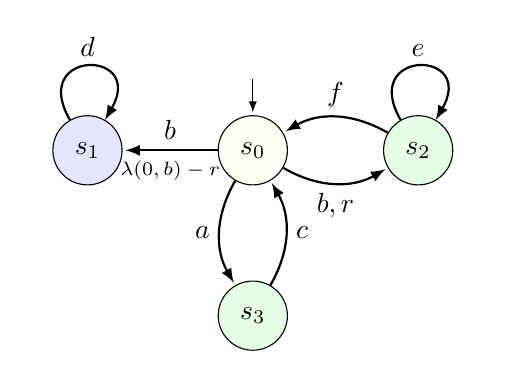
\begin{tikzpicture}[shorten >=1pt]
\begin{scope}
\node (l0) [state,ellipse,initial above, fill = safecellcolor]   {$s_0$};
\node (l1) [state, ellipse, fill = badcellcolor] at (-2.1,0)   {$s_1$};
\node (l2) [state, ellipse, fill = goodcellcolor] at (2.1,0)   {$s_2$};
\node (l3) [state,ellipse, fill = goodcellcolor] at (0,-2.1)   {$s_3$};
% \end{scope}
% \begin{scope}[every node/.style={scale=0.8}]

% \draw[rounded corners,->, thick] (l3) -- (-4.5,-4.3) -- node [below] {$b,(\lambda(0,b){-}r)$}  (l5);
\path [->, thick,above=.5cm,align=center]
    (l0) edge node [above] {$b$} node [below, font = \scriptsize]{$\lambda(0,b)-r$}   (l1)
    (l0) edge [bend right]  node [below] {$b,r$}   (l2)
    (l2) edge [bend right]  node [above] {$f$}   (l0)
    (l0) edge [bend right]  node [left] {$a$}   (l3)
    (l3) edge [bend right]  node [right] {$c$}   (l0)
    (l1) edge [loop above]  node [above] {$d$} ()
    (l2) edge [loop above]  node [above] {$e$} ()
    ;
\end{scope}
\end{tikzpicture}     
  \end{minipage}
  }
  \noindent\resizebox{0.3\textwidth}{!}{
  \begin{minipage}{0.33\textwidth}
   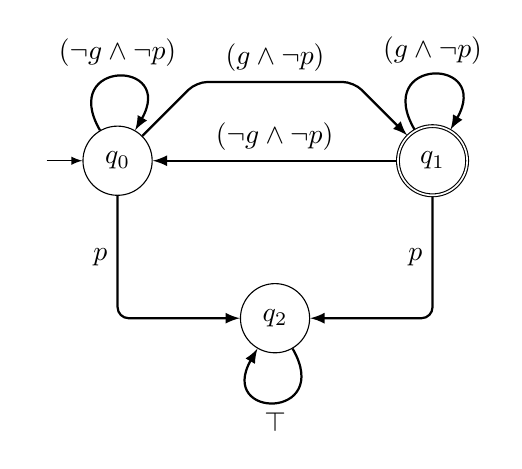
\begin{tikzpicture}
    \begin{scope}
    \node (l2) [state] {$q_2$};
    \node (l0) [state,initial] at (-2,2)   {$q_0$};
    \node (l1) [state,accepting] at (2,2)   {$q_1$};
    
\draw[rounded corners,->, thick] (l0) -- (-1, 3) -- node [above] {$(g \land \neg p)$} (1, 3) -- (l1);
\draw[->, thick] (l1) --  node [above] {$(\neg g \land \neg p)$} (l0);
\draw[rounded corners,->, thick] (l0) --  node [left] {$p$} (-2, 0) -- (l2);
\draw[rounded corners,->, thick] (l1) --  node [left] {$p$} (2, 0) -- (l2);
\path [->,thick]
    (l1) edge [loop above] node [above] {$(g \land \neg p)$} () 
    (l2) edge [loop below] node [below] {$\top$} ()
    (l0) edge [loop above] node [above] {$(\neg g \land \neg p)$}   ();
\end{scope}
\end{tikzpicture}
 \end{minipage}
 }
 \noindent\resizebox{0.3\textwidth}{!}{
\begin{minipage} {0.33\textwidth}
\centering
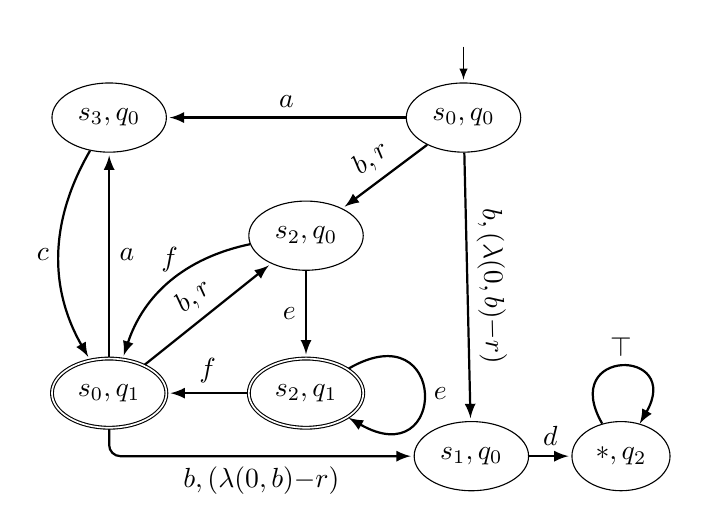
\begin{tikzpicture}[shorten >=1pt]
\begin{scope}
\node (l0) [state,ellipse,initial above]   {$s_0,q_0$};
\node (l1) [state, ellipse] at (-2,-1.5)   {$s_2,q_0$};
\node (l2) [state, ellipse] at (-4.5,0)   {$s_3,q_0$};
\node (l3) [state,ellipse,accepting] at (-4.5,-3.5)   {$s_0,q_1$};
\node (l4) [state,ellipse,accepting] at (-2,-3.5)   {$s_2,q_1$};
\node (l5) [state, ellipse] at (0.1,-4.3)   {$s_1,q_0$};
\node (l6) [state,ellipse] at (2,-4.3)   {$*,q_2$};
\draw[rounded corners,->, thick] (l3) -- (-4.5,-4.3) -- node [below] {$b,(\lambda(0,b){-}r)$}  (l5);
\path [->, thick,above=.5cm,align=center]
    (l0) edge node [above, sloped] {$b,r$}   (l1)
    (l0) edge  node [above] {$a$}   (l2)
    (l0) edge node [above,sloped] {$b,(\lambda(0,b){-}r)$}   (l5)
    (l2) edge [bend right] node [left] {$c$} (l3)
    (l3) edge  node [right] {$a$} (l2)
    (l3) edge node [above, sloped] {$b,r$} (l1)
    (l1) edge [bend right] node [above] {$f$} (l3)
    (l1) edge  node [left] {$e$} (l4)
    (l4) edge node [above] {$f$} (l3)
    % (l3) edge node [below] {$b,(\lambda(0,b){-}r)$} (l5)
    (l5) edge  node [above] {$d$} (l6)
    (l6) edge [loop above]  node [above] {$\top$} ()
    (l4) edge [loop right] node [right] {$e$} ()
    ;
\end{scope}
\end{tikzpicture}

  \end{minipage}
  }
% }
  \caption{The mars surveillance example where a CTMDP (left) can be in four different states where states $s_0$ has the label $\{\neg \mathtt{p} , \neg \mathtt{g}\}$, state $s_2$ and $s_3$ have label $\{\neg \mathtt{p}, \mathtt{g} \}$, and state $s_1$ have the label $\{\mathtt{p} ,\neg \mathtt{g}\}$. 
The rates of each transition (if not $1$) is written in the figure. 
  A deterministic B{\"u}chi automata for the $\omega$-regular objective $\varphi = (\always \neg \mathtt{p}) \wedge (\always\eventually \mathtt{g})$ (center). Product CTMDP (right) where each zone has two components for denoting the CTMDP and the B{\"u}chi automaton parts. All the zones whose second component is $q_2$ is combined as one. 
%   The accepting zones are coloured in green.
  The exit rate of an action from a zone $(s,q_i)$ in the product CTMDP is same as the exit rate of the action from $s$ in the original CTMDP. 
%   For example, the rate of action $b$ from zone $(0,q_0)$ is $\lambda(0,b)$.
}
 \label{fig:grid-world}
\end{figure*}

% \begin{tikzpicture}[shorten >=1pt]
% \begin{scope}
% \node (l0) [state,ellipse,initial above, fill = safecellcolor]   {$q_0$};
% \node (l1) [state, ellipse, fill = badcellcolor] at (-2.1,0)   {$q_1$};
% \node (l2) [state, ellipse, fill = goodcellcolor] at (2.1,0)   {$q_2$};
% \node (l3) [state,ellipse, fill = goodcellcolor] at (0,-2.1)   {$q_3$};
% % \end{scope}
% % \begin{scope}[every node/.style={scale=0.8}]

% % \draw[rounded corners,->, thick] (l3) -- (-4.5,-4.3) -- node [below] {$b,(\lambda(0,b){-}r)$}  (l5);
% \path [->, thick,above=.5cm,align=center]
%     (l0) edge node [above] {$b$} node [below, font = \scriptsize]{$\lambda(0,b)-r$}   (l1)
%     (l0) edge [bend right]  node [below] {$b,r$}   (l2)
%     (l2) edge [bend right]  node [above] {$f$}   (l0)
%     (l0) edge [bend right]  node [left] {$a$}   (l3)
%     (l3) edge [bend right]  node [right] {$c$}   (l0)
%     (l1) edge [loop left]  node [left] {$d$} ()
%     (l2) edge [loop right]  node [right] {$e$} ()
%     ;
% \end{scope}
% \end{tikzpicture}
 % \begin{tikzpicture}[scale=1.3,action/.style={->,very thick},
 %          cell name/.style={circle,fill=black,text=white,inner sep=1pt}]
 %        \coordinate (t1) at (0,0);
 %        \coordinate (t2) at ($ (t1) + (2,0) $);
 %        \coordinate (t3) at ($ (t1) + (60:2) $);
 %        \coordinate (c0) at ($ (t1) + (2,{2/sqrt(3)}) $);
 %        \foreach \x in {1, 2, 3} {
 %          \pgfmathparse{\x == 1 ? "badcellcolor" : "goodcellcolor"}
 %          \edef\cellcolor{\pgfmathresult}
 %          \path[fill=\cellcolor] (t\x) -- ++(2,0) -- ++(120:2) --cycle;
 %          \coordinate (c\x) at ($ (t\x) + (1,{1/sqrt(3)}) $);
 %        }
 %        % Cell contours.
 %        \draw[thick] (0,0) -- ++(4,0) -- ++(120:4) --cycle;
 %        \draw[fill=safecellcolor] (2,0) -- ++(60:2) -- ++(-2,0) --cycle;
 %        % Cell names.
 %        \node[cell name] at ($ (t1) + (2,3) $) {$3$};
 %        \node[cell name] at ($ (t2) + (0,1.2) $) {$0$};
 %        \node[cell name] at ($ (t1) + (1,1.2) $) {$1$};
 %        \node[cell name] at ($ (t2) + (1,1.2) $) {$2$};
 %        % Actions.
 %        \draw[action] ($ (c0) + (0.1,0.3) $) -- node[pos=0.15,right] {$a$} +(0,0.9);
 %        \draw[action] ($ (c0) - (0,0.2) $) -- node[pos=0.4,right]
 %             {$b$} ++(0,-0.5) -- node[at end,below,black] {$\lambda(0,b){-}r~$} ++(-0.7,0);
 %             \draw[action] ($ (c0) - (0,0.2) $) ++(0,-0.5) --
 %             node[at end,below,black] {$r~~~$} ++(0.7,0);
 %             \draw[action] ($ (c3) - (0.1,0) $) -- node[pos=0.25,left] {$c$} +(0,-0.9);
 %            %  \draw[action] (c1) -- node[pos=0.1,above] {$d$} ++(30:0.9);
 %             \draw[action] ($ (c1) + (215:0.5) $)            arc[radius=0.4cm,start angle=390,end angle=45] node[at start,left] {$~d$};
 %             \draw[action] ($ (c2) + (-45:0.5) $)
 %             arc[radius=0.4cm,start angle=150,end angle=490] node[at start,right] {$e$};
 %             \draw[action] (c2) -- node[pos=0.1,above] {$f$} ++(150:0.9);
 %      \end{tikzpicture}
% Given the unknown uncertainty of the terrain of Mars, the system is modeled as a CTMDP with associated uncertainty on the time of various actions where the exit rate of action $a$ from Zone (state) $0$ is denoted by $\lambda(0,a)$. In other words, when selected an action $a$ in a state $s$, the probability of spending $t$ time units in $s$ before taking $a$ is given by the cumulative distribution function $1 - e^{- \lambda(0,a)t}$.
% Assume that the action $b$ from Zone $0$ goes to Zone $2$ with rate $r$ (high probability) and to Zone $1$ with rate  $(\lambda(0,b) - r)$ (low probability).

% The mission objective is to avoid Zone $1$ (blue zone) while infinitely often visiting the Zone $2$ or $3$ (the green zones). 
% It can be captured in LTL~\cite{Baier08} as:
% \[
% \varphi = (\always \neg \mathtt{b}) \wedge (\always(\eventually \mathtt{g}))
% \]
% specifying that across the infinite horizon {\bf globally} (i.e. at every step expressed as temporal modality, $\always$) avoid the blue region ($\neg b$), and globally {\bf finally} (i.e. at some time in the future expressed as temporal modality, $\eventually$) reach the green region, i.e. $(\always (\eventually g))$. 
% The $GF \phi$ modality is often referred as \emph{infinitely often $\phi$}.
% LTL combines these temporal operators using the standard propositional logic connectives such as: and ($\wedge$), or ($\lor$), not ($\neg$), and implication ($\to$).

% This declarative specification can also be expressed using the B\"uchi automaton shown in Figure~\ref{fig:grid-world} (center) where the double circled states (here, $q_1$) denote accepting states.
% The B\"uchi automata can be used as the monitors of the behaviors of the learner over the environments given as CTMDPs. For our example, it is visualized by taking the synchronous product (an extended space CTMDP) of the CTMDP with the automaton shown in Figure~\ref{fig:grid-world} (right).

% For the satisfaction semantics on the product CTMDP, our goal is to maximize the probability that every infinite horizon behavior visits the accepting state infinitely often, while for the expectation semantics the goal is to maximize the expected time the system dwells in the final state.
% \begin{itemize}
%     \item \noindent {\bf Satisfaction Objective.} 
% Consider the case where we have one Mars rover in this mission. Hence, our goal naturally is to maximize the probability of visiting green zones infinitely often while avoiding the blue zone (the satisfaction semantics).
% In this case, the optimal schedule is to choose actions $a$ and $c$ indefinitely, i.e. the schedule $(a \to c)^\omega$, that satisfies the objective with probability $1$.
% Note that it does not make sense to choose action $b$ no matter how low the probability is to reach the blue zone.
% \item 
% \noindent {\bf Expectation Objective.} Consider an alternative setting where we have a fleet of drones (we are okay is losing some drones as long as we maximize the mission objective) that needs to be sent to the surveillance of zone $2$ or $3$. 
% Suppose that due to unforeseeable circumstances the mission may cease operation any time, and hence the goal is to maximize total expected time spent in the green zones ($2$ and $3$).
% The schedule $(a\to c)^\omega$ is not optimal anymore as it may dwell a considerable amount in the Zone $0$. 
% On the hand hand any drone that chooses $b$ in Zone $0$ risks moving to Zone $1$ with a small probability.
% As our goal is to maximize the expected time over a large group of drones, the expectation semantics captures this intent and the optimal schedule is to start with action $b$.
% \end{itemize}
% \end{example}

% \section{Good-for-CTMDP B\"uchi Automata}
% \label{app:gfm}
% \paragraph{Product CTMDP.}
%  Given a \emph{labelled} CTMDP $(\Mdp, \atomicprop, \labelling)$ where $\atomicprop$ is a set of atomic propositions, and $\labelling: \states \rightarrow 2^\atomicprop$ is a labelling function and a   B{\"u}chi automaton $\oautomata = (2^{\atomicprop}, \ostate, \oinitstate, \otrans, \acceptingc)$, the product CTMDP is defined as $\Mdp \times \oautomata = ((\states \times \ostate),(\initstate,\oinitstate),\actions,\transR^{\times},\acceptingc^{\times})$ where the rates are $\transR^{\times} : (\states \times \ostate) \times \actions \times (\states \times \ostate) \rightarrow \Reals_{\geq 0}$ such that $\transR^{\times} ((s,q),a,(s',q') = \transR(s,a,s')$ if $\transR(s,a,s')>0$ and $\otrans (q,\labelling(s)) = \{q'\}$.
% If $F$ is the set of accepting 
% % transitions 
% states
% in $\oautomata$, then the accepting condition is a set 
% % transitions $F^\times$ where $((s,q),a,(s',q')) \in F^\times$ iff $(q,\labelling(s),q') \in F$ 
% $F^\times$ of states where $(s,q) \in F^\times$ iff $q \in F$. An example of a product CTMDP is given in Figure~\ref{fig:grid-world}.  

% Given an MDP $\Mdp$, a B\"uchi automaton  $\oautomata$, and product $\Mdp \times \oautomata$, we define the following two  problems:
% \begin{enumerate}
%     \item {\bf Satisfaction Semantics.} 
%     Compute a schedule of $\Mdp$ that maximizes the probability of visiting final states $F$ of $\oautomata$ infinitely often.
%     We define the satisfaction probability $\PSat^{\Mdp \times \oautomata}(s, \sigma)$ of a schedule $\sigma$ from starting state $s$ as: 
% \begin{equation*}
% \Pr{}^{\Mdp \times \oautomata}_{\sigma}(s) \set{\forall_i  \exists_{j{\geq} i} [X_j \in F^\times] }.
% \end{equation*}
% The optimal satisfaction probability
% $\PSemSat^{\Mdp \times \oautomata}_{\oautomata}(s)$ for specification $\oautomata$ 
% is defined as $\sup_{\sigma \in \Sigma_{\Mdp \times \oautomata}} \Pr^{\Mdp \times \oautomata}_{\sigma}(s, \sigma)$ and we say
% that $\sigma$ is an optimal schedule for $\oautomata$ if
% $\PSemSat^{\Mdp \times \oautomata}_{\oautomata}(s, \sigma) (s) = \PSemSat^{\Mdp \times \oautomata}_{\oautomata}$.

% \item {\bf Expectation Semantics.} Compute a schedule of $\Mdp$ that maximize the long-run expected average time spent in the final states of $\oautomata$.
% We define the expected satisfaction time $\ESat^{\Mdp \times \oautomata}_{\oautomata}(s, \sigma)$ 
% of $\sigma$ from starting state $s$ as: 
% \begin{equation*}
%  \mathbb{E}^{\Mdp \times \oautomata}_{\sigma}(s) \set{ \liminf_{n \rightarrow \infty} \frac{\sum_{i=1}^{n} [X_i {\in} F] D_i}{T_n}}.
% \end{equation*}
% The optimal expected satisfaction time
% $\ESat^{\Mdp \times \oautomata}_{\oautomata}(s)$ for $\oautomata$ is defined as $\sup_{\sigma \in \Sigma_{\Mdp}} \ESat^{\Mdp \times \oautomata}_{\oautomata}(s, \sigma)$ and we say that $\sigma \in \Sigma_\Mdp$ is an optimal expected-satisfaction schedule for $\oautomata$ if
% $\ESat^{\Mdp \times \oautomata}_{\oautomata}(s, \sigma) = \ESat^{\Mdp \times \oautomata}_{\oautomata} (s)$.
% \end{enumerate}

% We call a B{\"u}chi automaton $\oautomata = (2^{\atomicprop}, \ostate, \oinitstate, \otrans, \acceptingc)$ good-for-CTMDP if for every \emph{labelled} CTMDP $(\Mdp, \atomicprop, \labelling)$ where $\atomicprop$ is a set of atomic propositions, we have that 
% \begin{eqnarray*}
%     \PSemSat^{\Mdp}_{\oautomata}(s, \sigma) &=&\PSat^{\Mdp \times \oautomata}_{\oautomata}(s, \sigma)~\text{ and }\\
%     \ESemSat{}^{\Mdp}_{\oautomata}(s, \sigma) &=&
%     \ESat^{\Mdp \times \oautomata}_{\oautomata}(s, \sigma).
% \end{eqnarray*}
% A good-for-CTMDP automaton allows the computation of the optimal schedule by solving the corresponding problem on the product CTMDP. 
% If a B\"uchi automata is good-for-MDP, then one can show via uniformization that it is also good-for-CTMDPs.
% There exists several syntactic characterizations of good-for-MDP automata including suitable limit-deterministic B\"uchi automata (SLDBA)~\cite{sickert2016limit} and slim automata~\cite{HPSS20}.
% Moreover, every LTL specification can be effectively converted into a GFM B\"uchi automata.

% % \begin{theorem}[Good-for-MDP B\"uchi Automata]
% % \end{theorem}

% \section{Blackwell Optimality In CTMDP}
% \label{sec:blackwell_optimality}
% % \subsection{Blackwell Optimality In CTMDP}
% \track{Though both of our semantics use different reward machines, for learning schedules for both objectives, we reduce the problem to maximising the expected average reward.
% We use off-the-shelf RL algorithms for learning the schedulers in both settings.}
% Standard RL algorithms try to optimise discounted payoff objective while 
% % as shown above, for the expectation semantics, 
% we need to optimise the expected average reward. Blackwell optimality allows us to use a schedule that optimises the expected discounted payoff with a high discount factor and such a schedule also optimises the expected average payoff.

% \vspace{0.5em}\noindent\textbf{Existence of Blackwell Optimal Schedules in CTMDP.} 
% We give a simple uniformization based proof on the existence of a Blackwell optimal pure schedule in a CTMDP.
In this section, we provide a uniformization based proof of Theorem~\ref{corollary:1}.
Consider a CTMDP $\Mdp$, a pure schedule $\sigma$, and a continuous-time discounting with parameter $\dfactor > 0$. 
% The one-step expected reward obtained from taking action $a \in \actions{}(s)$ from state $s \in \states$ is given by $\rho(s,a) = rew(s,a) + \frac{rew(s)}{\dfactor + \lambda(s,a)}$ (~$\!\!$\cite{puterman2014markov}~Eq 11.5.3). 
We define a function $\ctmdprate : \states \times \actions \rightarrow [0,1) $ where $\ctmdprate(s,a) = \frac{\lambda(s,a)}{\lambda(s,a) + \dfactor}$ where $\dfactor > 0$.
We call $\ctmdprate(s,a)$ the \emph{discount rate} of the state-action pair $(s,a)$ in $\Mdp$.
So, the expected discounted reward (also known as value of $s$) $\discobjective^{\Mdp[\sigma]} (\alpha)(s)$ is given by
% For a pure schedule $\sigma$, the value of a state $s$, denoted by $\valuesigma_{\ctmdprate(s,\sigma(s))}$,
% \track{CHANGE NOTATION} 
% is given by 
\begin{equation}\label{eq:7.1}
\begin{split}
     \rho(s,a_{\sigma}) + 
     \ctmdprate(s,a_{\sigma})
     \sum_{s' \in s} \pmtrx(s,a_\sigma,s') 
     \discobjective_{\sigma}^{\Mdp}(\alpha)(s')
\end{split}
\end{equation}
Consider a DTMDP $\mathcal{N}$, a schedule $\sigma$, and a discount rate $0\leq \drate < 1$. Let $\valuesigma_{\drate}(\mathcal{N},s)$ denote the total discounted value from state $s$ in $\mathcal{N}$ under schedule $\sigma$.

A pure schedule $\bschedule$ is \emph{Blackwell optimal} in $\mathcal{N}$ if there exists a threshold discount rate $0 \leq \thrate < 1$ such that for any discount rate $\thrate \leq \drate < 1$, we have $\valuestar_{\drate}(\mathcal{N},s) \geq \valuesigma_{\drate}(\mathcal{N},s)$ for all $\sigma \in \Sigma_{\mathcal{N}}$. It is known that a Blackwell optimal schedule maximises both discounted and average reward objectives in DTMDPs.
% From \cite{puterman2014markov}~Thm 10.1.4, we have,
% \begin{theorem}\label{puterman1}
From \cite{puterman2014markov}~(Thm 10.1.4), we have that for every DTMDP $\mathcal{N}$, there exists a Blackwell optimal \emph{pure} schedule $\bschedule$, and $\bschedule$ also maximises the average reward in $\mathcal{N}$.
% \end{theorem}
Now, given a CTMDP $\Mdp$, let $C$ be a constant such that $C \geq \lambda(s,a)$ for all state-action pairs in $\Mdp$. 
Let $\uMdp$ be the uniformized CTMDP of $\Mdp$ with constant exit rate $C$, and let $\upmtrx$ be the probability matrix of $\uMdp$. As the exit rate $\lambda(s,a) = C$ for all $s\in \states$ and $a \in \actions{}(s)$, we have that $\ctmdprate(s,a) = \frac{C}{C+\dfactor}$ for all state-action pairs. We denote this discount rate by $\udrate$. 
The value of a state $s$ under a schedule $\sigma$ in $\uMdp$, 
% \track{under schedule $\sigma$}
denoted $\discobjective^{\uMdp^{\sigma}}(\alpha)(s)$
% $\valuesigma_{\udrate}(\uMdp,s)$ 
is given by, 
\begin{equation}\label{eq:7.2}
     \Bar{\rho}(s,a_\sigma) + \udrate \sum_{s' \in s} \upmtrx(s,a_\sigma,s') \discobjective^{\uMdp^{\sigma}}(\alpha)(s')
\end{equation}
where $\Bar{\rho}(s,a) = \rho(s,a)\cdot \frac{\dfactor + \lambda(s,a)}{\dfactor + C} $. 
We extend the above result of existence of Blackwell optimal schedules in DTMDPs to uniform CTMDPs.
\begin{lemma} \label{lemma:1}
For a uniform CTMDP $\uMdp$, there exists a Blackwell optimal schedule $\bschedule$. Further, $\bschedule$ also maximises the expected average reward in $\uMdp$.
\end{lemma}
\begin{proof}
Consider a DTMDP $\mathcal{N}$ with the same set of states as that of $\uMdp$, one step reward function $\Bar{r}$ and probability matrix $P_{\mathcal{N}} = \upmtrx$. For a pure schedule $\sigma$ and a discount rate $0 \leq \drate < 1$, the value of a state $s$ in $\mathcal{N}$ is 
\begin{equation}\label{eq:7.3}
    \valuesigma_{\drate}(\mathcal{N},s) = \Bar{r}(s,\sigma(s)) + \drate \sum_{s' \in s} \upmtrx(s,\sigma(s),s') \valuesigma_{\drate}(\mathcal{N},s')
\end{equation}
We observe that equation \ref{eq:7.3} is identical to equation \ref{eq:7.2} when $\udrate = \drate$. Therefore, the set of equations defining the values of states in $\mathcal{N}$ and $\uMdp$ are identical. Let this set be denoted by $E^\sigma$. From \cite{puterman2014markov}~Thm 6.1.1, we know that for each stationary schedule $\sigma$, there exists a unique solution for $E^\sigma$. The set of pure schedules in $\uMdp$ and $\mathcal{N}$ are equal as the set $S$ of states and the set $\av$ of available actions from each state are the same for both.\\*
Therefore, for a pure schedule $\sigma$, and discount rates $0 \leq \drate = \udrate < 1$, we have
\begin{equation}\label{eq:7.4}
    \valuesigma_{\udrate}(\uMdp,s) = \valuesigma_{\drate}(\mathcal{N},s) \text{\: for $\udrate = \drate$, for all states $s$}
\end{equation}
From Theorem~10.1.4 in \cite{puterman2014markov}, we know that in $\mathcal{N}$, there exist a Blackwell optimal pure schedule $\sigma^*$, and a threshold discount rate $\thrate$ such that 
\begin{align}\label{eq:7.5}
 \valuestar_{\drate}(\mathcal{N},s) \geq \valuesigma_{\drate}(\mathcal{N},s)   
\end{align}
for all $\sigma \in \Sigma_{N}$ and $\thrate \leq \drate < 1$.\\
From equations \ref{eq:7.4} and \ref{eq:7.5} we can conclude that 
\begin{equation}\label{eq:7.60}
    \valuestar_{\udrate}(\uMdp,s) \geq \valuesigma_{\udrate}(\uMdp,s)   
\end{equation}
for all $\sigma \in \Sigma_{\uMdp}^{pure}$ and $\thrate \leq \udrate < 1$.\\
From \cite{puterman2014markov}~Thm 11.5.2(d), we know that there exists an optimal pure schedule maximising the discounted reward in a CTMDP. Therefore,
\begin{equation}\label{eq:7.}
    \valuestar_{\udrate}(\uMdp,s) \geq \valuesigma_{\udrate}(\uMdp,s)   
\end{equation}
for all $\sigma \in \Sigma_{\uMdp}$ and $\thrate \leq \udrate < 1$.\\
A similar argument can be made to show that $\sigma^*$ also maximises the expected average reward in $\uMdp$.
\end{proof}

The above lemma proves the existence of a Blackwell optimal schedule in uniform CTMDPs. 
We further extend this result to general CTMDPs which is the main result of this section.

\begin{lemma}\label{lemma:2}
If $\sigma^*$ is a Blackwell optimal pure schedule in $\uMdp$, then it is also Blackwell optimal in $\Mdp$.
\end{lemma}
\begin{proof}
Since $\bstrategy$ is a Blackwell optimal pure schedule in $\uMdp$, there exists a threshold discount rate $\uthrate$ such that for all $\uthrate \leq \udrate < 1$, we have that 
\begin{equation}\label{eq:7.7}
    \valuestar_{\udrate}(\uMdp,s) \geq \valuesigma_{\udrate}(\uMdp,s)   
\end{equation}
for all $\sigma \in \Sigma_{\uMdp}$.\\
The set of pure schedules in $\Mdp$ and $\uMdp$ are the same. From \cite{puterman2014markov}~Thm 11.5.2(d), we know that there exists an optimal pure schedule maximising the discounted reward in $\Mdp$. \cite{puterman2014markov}~Prop 11.5.1, states that for every pure schedule $\sigma$ and a state $s$, we have that  
\begin{equation}\label{eq:7.8}
    \valuesigma_{\ctmdprate(s,\sigma(s))}(\Mdp,s) = \valuesigma_{\udrate}(\uMdp,s)   
\end{equation}
If $\uthrate = \frac{C}{C+\dfactor}$ is the threshold discount rate in $\uMdp$, then the corresponding threshold discount rate for a state $s$ in $\Mdp$ is given by 
$\ctmdpthrate(s,a) = \frac{\lambda(s,a)}{\lambda(s,a)+\dfactor_{o}}$.\\
From equations \ref{eq:7.7} and \ref{eq:7.8}, we can conclude that for each state $s$ in $\Mdp$, there exist a pure schedule $\bstrategy$, and a threshold discount rate $\ctmdpthrate(s,\bstrategy(s)) $ such that for all $\ctmdpthrate(s,\bstrategy(s)) \leq \ctmdprate(s,\bstrategy(s)) < 1$, we have that
\begin{equation}\label{eq:7.9}
    \valuestar_{\ctmdprate(s,\bstrategy(s))}(\Mdp,s) \geq \valuesigma_{\ctmdprate(s,\sigma(s))}(\Mdp,s)   
\end{equation}
for all $\sigma \in \Sigma_{\Mdp}$.
As the set of states is finite in $\Mdp$, the threshold discount rate for $\Mdp$ is given by
    $\ctmdpthrate^{\Mdp} = \max_{(s,a) \in \states \times \actions} \ctmdpthrate(s,a)$.
\end{proof}
Thus, any Blackwell optimal schedule $\bstrategy$ in $\uMdp$ is also Blackwell optimal in $\Mdp$. The following lemmas show that $\sigma^*$ also maximises the expected average reward.
\begin{lemma}\label{lemma:3}
An optimal schedule maximising the expected average reward in $\uMdp$ also maximises the expected average reward in $\Mdp$.
\end{lemma}
\begin{proof}
For a pure schedule $\sigma$ , the expected average reward in $\Mdp$ is denoted by $\avgrew^{\sigma}(\Mdp)$. From \cite{puterman2014markov}~Chap 11.5.3, we observe that for a pure schedule $\sigma$, 
\begin{equation}\label{eq:7.10}
    \avgrew^{\sigma}(\Mdp) = \avgrew^{\sigma}(\uMdp)\cdot C 
\end{equation}
Let $\sigma'$ be a pure schedule maximising the expected average reward in $\uMdp$, i.e, 
\begin{equation}\label{eq:7.11}
 \avgrew^{\sigma'}(\uMdp) = \sup_{\sigma \in \Sigma_{\uMdp}} \avgrew^{\sigma}(\uMdp)
\end{equation}
The set of pure schedules in $\Mdp$ and $\uMdp$ are equal and we know that there exists a pure schedule maximising the average reward in a CTMDP (\cite{puterman2014markov}~Thm 11.4.6(d)). Therefore, from equations \ref{eq:7.10} and \ref{eq:7.11} we can conclude that, 
\begin{equation}\label{eq:7.12}
    \avgrew^{\sigma'}(\Mdp) = \sup_{\sigma \in \Sigma_{\Mdp}} \avgrew^{\sigma}(\Mdp)
\end{equation}
Therefore, $\sigma'$ is an optimal schedule maximising the average reward in $\Mdp$.
\end{proof}
\begin{lemma}\label{lemma:4}
A Blackwell optimal schedule $\bstrategy$ in $\Mdp$ also maximises the average reward in $\Mdp$.
\end{lemma}
\begin{proof}
From Lemma \ref{lemma:1}, we know that $\bstrategy$ is an optimal schedule maximising the expected average reward in $\uMdp$. Lemma \ref{lemma:3} shows that if $\bstrategy$ is an optimal schedule maximising the expected average reward in $\uMdp$ then $\bstrategy$ also maximises the expected average reward in $\Mdp$. Therefore, we can conclude that $\bstrategy$ is an optimal schedule maximising the expected average reward in $\Mdp$.
\end{proof}
Lemma~\ref{lemma:2} and Lemma~\ref{lemma:4} gives us the following.
\paragraph{Theorem~\ref{corollary:1}.}For a CTMDP $\Mdp$, there exists a Blackwell optimal pure schedule $\bschedule$ and a threshold $0 \leq \ctmdpthrate^{\Mdp} < 1$ such that :
\begin{inparaenum}[(1).]
    \item For any discount-rate function $\ctmdprate$ where $\ctmdprate(s,a) \geq \ctmdpthrate^{\Mdp}$ for all valid state-action pairs $(s,a)$, the schedule $\bschedule$ is an optimal schedule maximising the expected discounted reward.
    \item The schedule $\bschedule$ also maximises the expected average reward.
\end{inparaenum}
% \paragraph{Theorem ~\ref{corollary:1}}
% For a CTMDP $\Mdp$, there exists a Blackwell optimal pure schedule $\bschedule$ and a threshold $0 \leq \ctmdpthrate^{\Mdp} < 1$ such that :
% \begin{inparaenum}[(1).]
%     \item For any discount-rate function $\ctmdprate$ where $\ctmdprate(s,a) \geq \ctmdpthrate^{\Mdp}$ for all valid state-action pairs $(s,a)$, the schedule $\bschedule$ is an optimal schedule maximising the expected discounted reward.
%     \item The schedule $\bschedule$ also maximises the expected average reward.
% \end{inparaenum}

% \begin{proof}[Proof sketch]
% % \begin{lemma}\label{lemma:2}
% Note that the set of pure schedules are the same in $\Mdp$ and $\uMdp$.
% First we prove that if $\bschedule$ is a Blackwell optimal pure schedule in $\uMdp$, then it is also Blackwell optimal in $\Mdp$. 
% This is done using the fact that the value of each state in $\uMdp$ and $\Mdp$ are equal (Prop 11.5.1 in \cite{puterman2014markov}) i.e, for every pure schedule $\sigma$ and a state $s$, we have that
% \[
% \discobjective^{\ctmc} (\alpha)(s) = \discobjective^{\uMdp^{\sigma}}(\alpha)(s)
% \] 
% % \track{ELABORATE}
% From this equation, we can get the threshold discount rate satisfying the Blackwell optimality condition for $\Mdp$.
% % \end{lemma}
% Thus, we conclude that any Blackwell optimal schedule $\sigma^*$ in $\uMdp$ is also Blackwell optimal in $\Mdp$. 
% % The following lemmas show that $\sigma^*$ also maximises the expected average reward in $\Mdp$.

% Next we show that 
% % \begin{lemma}\label{lemma:3}
% an optimal schedule maximising the expected average reward in $\uMdp$ also maximises the expected average reward in $\Mdp$. 
% For a given pure schedule $\sigma$, we denote the expected average reward in $\Mdp$ and $\uMdp$ from a state $s$ by $\avgobjective^{\Mdp^{\sigma}}(s)$ and $\avgobjective^{\uMdp^{\sigma}}(s)$
% % \track{WE ALREADY HAVE NOTATIONS FOR EXPECTED AVERAGE REWARD} 
% respectively.
% From Section~11.5.3 in \cite{puterman2014markov}, we get the following result:
% \[
% \avgobjective^{\Mdp^{\sigma}}(s) = \avgobjective^{\uMdp^{\sigma}}(s)\cdot C \] 
% % This is due to the fact that 
% % the expected average reward obtained by a schedule in $\uMdp$ is directly proportional to the expected average obtained by the same schedule in $\Mdp$, . \track{ELABORATE}
% From this equation, we have that if a pure schedule maximises the expected average reward in $\uMdp$, it also maximises the expected average reward in $\Mdp$.
% % Therefore, optimal pure schedules maximising the expected average reward in $\Mdp$ and $\uMdp$ are the same. 
% % Now we prove the following lemma.

% In Lemma~\ref{lemma:1}, we have shown the existence of a pure Blackwell optimal schedule $\bschedule$ in $\uMdp$ and it also maximises the expected average reward. 
% From the above results we obtain that $\bschedule$ also is Blackwell optimal and maximises the expected average reward in $\Mdp$.
% % Finally, using Lemma~\ref{lemma:1}, we show that a Blackwell optimal schedule $\bschedule$ in $\Mdp$ also maximises the average reward in $\Mdp$. \track{ELABORATE}
% % We can get this result directly from Lemma~\ref{lemma:1}.
% % \end{lemma}
% % Lemma \ref{lemma:2} and Lemma \ref{lemma:4} give us the following.
% % \begin{corollary}\label{corollary:1}
% % For a CTMDP $\Mdp$, there exists a Blackwell optimal pure schedule $\bschedule$ and a threshold $0 \leq \ctmdpthrate^{\Mdp} < 1$ such that :
% % \begin{inparaenum}[(1).]
% %     \item For any discount-rate function $\ctmdprate$ where $\ctmdprate(s,a) \geq \ctmdpthrate^{\Mdp}$ for all valid state-action pairs $(s,a)$, the schedule $\bschedule$ is an optimal schedule maximising the expected discounted reward.
% %     \item The schedule $\bschedule$ also maximises the expected average reward.
% % \end{inparaenum}
% % \end{corollary}
% \end{proof}

% \track{ In the following sections, we design reward functions for specific objectives such that a schedule maximising the expected average reward will also maximise the given objective. As standard RL algorithms optimise discounted reward objectives, we use the result from Theorem~\ref{corollary:1} to conclude that for a large enough discount factor, the RL algoirithm will synthesise the optimal schedule. }

\begin{comment}
\vspace{0.5em}\noindent\textbf{Algorithm for Expectation Semantics.} We show the procedure to obtain an optimal schedule $\sigma$ for expectation semantics in Algorithm \ref{algo:expt}.  Line 1 initialises the Q-function for reinforcement learning. Here, the Q-function is defined on the states of the product CTMDP i.e, $Q_f: (\states \times Q) \times \actions \rightarrow \mathbb{R}$ where $\states$ is the set of states of the CTMDP $\Mdp$ and $Q$ is the set of states of the \textbf{GFM} $A$.
% Variable $i$ keeps track of the number of episodes completed and variable $j$ keeps track of the length of an episode.
The number of episodes to be conducted and the length of the episode is defined by the user and is stored in $k$ and $eplen$ respectively.
The variables $s$ and $q$ represents the current state of $\Mdp$ and $A$ respectively and is initialised to their initial states. The action $a$ from the current state of CTMDP and the transition $t$ from the state of GFM is picked according to the RL policy used (eg. $\epsilon$-greedy). We observe the next state $(s',q')$ and the time spent $\tau$ in the current state. The reward function $R'$ is defined based on $r'$ defined previously. For a given state $(s,q)$ and action $a$, if $\tau$ is the observed time spent in $(s,q)$ then,
$$
 R'((s,q),a,\tau) = \begin{cases}
 \tau & \text{if ($s,q$) is an accepting state}\\
 0 & \text{otherwise}
 \end{cases}
 $$
Variable $r$ stores the reward obtained in each iteration of the episode. The Q-function is updated according to the Q-learning rule defined in section \ref{prelims}. An episode ends when the length of the episode reaches $eplen$. After the completion of $k$ episodes, we obtain the optimal schedule $\sigma$ by choosing the action that gives the highest Q-value from each state.

\begin{algorithm}[t]
\caption{Algorithm for expectation semantics}\label{algo:expt}
\hspace*{\algorithmicindent} \textbf{Input:}  \text{Initial state $s_{init}$, GFM $A$, discount factor $\gamma$,}\\
\hspace*{\algorithmicindent} \hspace{11mm}\text{reward function $R'$, number of episodes $k$,} \\
\hspace*{\algorithmicindent}\hspace{11mm} \text{learning rate $\alpha$, episode length $eplen$}\\
\hspace*{\algorithmicindent} \textbf{Output:}  \text{Optimal schedule $\sigma$}
\begin{algorithmic}[1]
\STATE Initialise $Q_f$ to all zeroes
% \STATE $i \leftarrow 0$
\FOR{$k$ episodes}
\STATE Initialise $s$ and $q$ to $s_0$ and $q_0$ respectively
% \STATE $q \leftarrow q_0$
% \STATE $r \leftarrow 0$
% \STATE $j \leftarrow 0$
\FOR{each episode}
\STATE Choose action $a$ using policy derived from $Q$ 
\STATE Take action $a$, observe next state $s'$, and time $\tau$
\STATE Choose non-deterministic transition $t$ in $A$ using the derived policy
\STATE Take transition $t$ in $A$, observe next state $q'$
\STATE $r \leftarrow R'(s,q,a,\tau)$
\STATE $V(s',q') \leftarrow \max\limits_{a' \in \actions} Q_f(s',q',a')$
\STATE $Q_f(s,q,a) {\leftarrow} (1-\alpha) Q_f(s,q,a)  {+}\alpha \bigl(r {+} e^{-\gamma\tau} V(s',q') \bigr)$
\STATE $s \leftarrow s'$; $q \leftarrow q'$
% \STATE $q \leftarrow q'$
% \STATE $j \leftarrow j+1$
\ENDFOR
% \STATE $i \leftarrow i+1$
\ENDFOR
\FOR{Each state (s,q)}
\STATE $\sigma(s,q) = \max_{a \in \actions}Q(s,q,a)$
\ENDFOR
\end{algorithmic}
\end{algorithm}
\end{comment}


% % \begin{center}
% %     {\Large Appendix}
% % \end{center}
% % \section{Appendix}
% % \section{Appendix for Proofs}

\paragraph{Proof of Theorem \ref{thm:main}.}

\begin{proof}
\label{proof:main}
Our proof has two steps. In Step 1, we will show that SimCLR is equivalent to minimizing the cross entropy loss defined in Eqn.~(\ref{eqn:cross-entropy}). 
In Step 2, we will show  that minimizing the cross-entropy loss 
is equivalent to spectral clustering on $\bfpi$. 
Combining the two steps together, we have proved our theorem. 

\textbf{Step 1: } SimCLR is equivalent to minimizing the cross entropy loss.

The cross-entropy loss takes expectation over 
$\bfW_\bfX\sim \mathbb{P}(\cdot ; \bfpi)$, 
which means $\bfW_\bfX$ has exactly one non-zero entry in each row $i$. By Lemma~\ref{lem:multinomial}, we know every row $i$ of $\bfW_\bfX$ is independent of other rows. Moreover, 
$\bfW_{\bfX,i}\sim \mathcal{M}(1, \bfpi_i/\sum_j \bfpi_{i,j})=\mathcal{M}(1, \bfpi_i)$, because $\bfpi_i$ itself is a probability distribution.
Similarly, we know $\bfW_\bfZ$ also has the row-independent property by sampling over $\mathbb{P}(\cdot;\bfK_\bfZ)$.
Therefore, by Lemma~\ref{lem:cross_split}, we know Eqn.~(\ref{eqn:cross-entropy}) is equivalent to:
\[
 -\sum_{i=1}^n \mathbb{E}_{\bfW_{\bfX,i}}[\log \mathbb{P}(\bfW_{\bfZ,i}=\bfW_{\bfX,i};\bfK_\bfZ)],
\]

This expression takes expectation over $\bfW_{\bfX,i}$ for the given row $i$. Notice that 
$\bfW_{\bfX,i}$ has exactly one non-zero entry, which equals $1$ (same for $\bfW_{\bfZ,i}$). 
As a result
we expand the above expression to be:
\begin{equation}
 -\sum_{i=1}^n \sum_{j\neq i} \Pr(\bfW_{\bfX,i,j}=1)\log \Pr(\bfW_{\bfZ,i,j}=1).
\label{eqn:detailed-expansion}    
\end{equation}


By Lemma~\ref{lem:multinomial}, $\Pr(\bfW_{\bfZ,i,j}=1)=\bfK_{\bfZ,i,j}/\|\bfK_{\bfZ,i}\|_1$ for $j\neq i$. Recall that $\bfK_\bfZ=(k(\bfZ_i-\bfZ_j))_{(i,j)\in[n]^2}$, which means 
$\bfK_{\bfZ,i,j}/\|\bfK_{\bfZ,i}\|_1=\frac{\exp(-\|\bfZ_i-\bfZ_j\|^2/{2\tau})}{\sum_{k\neq i}
\exp(-\|\bfZ_i-\bfZ_k\|^2/{2\tau})
}$ for $j\neq i$, when $k$ is the Gaussian kernel with variance $\tau$. 

Notice that $\bfZ_i=f(\bfX_i)$, so we know
\begin{equation}
-\log \Pr(\bfW_{\bfZ,i,j}=1)=
-\log \frac{\exp(-\|f(\bfX_i)-f(\bfX_j)\|^2/{2\tau})}{\sum_{k\neq i}
\exp(-\|f(\bfX_i)-f(\bfX_k)\|^2/{2\tau}),
}
\label{eqn:infonce-equivalence}    
\end{equation}


The right hand side is exactly the InfoNCE loss defined in Eqn.~(\ref{eqn:infonce}).
Inserting Eqn.~(\ref{eqn:infonce-equivalence}) into Eqn.~(\ref{eqn:detailed-expansion}), we get the SimCLR algorithm, which first samples augmentation pairs $(i,j)$ with $\Pr(\bfW_{\bfX,i,j}=1)$ for each row $i$, and then optimize the InfoNCE loss. 

\textbf{Step 2: } minimizing the cross entropy loss 
is equivalent to spectral clustering on $\bfpi$.


By Lemma~\ref{lem:convert_to_spectral}, we may further convert the loss to 
\begin{equation}
\label{eqn:main-theorem-repul-attr}
\min_{\bfZ}
-\sum_{(i,j)\in [n]^2} \mathbf{P}_{i,j}
\log k (\bfZ_i-\bfZ_j)+\log \mathbf{R}(\bfZ).
\end{equation}
Since $k$ is the Gaussian kernel, this reduces to \[
\min_\bfZ \mathrm{tr}(\bfZ^\top \mathbf{L}(\bfpi) \bfZ)
+\log \mathbf{R}(\bfZ),
\]

where we use the fact that $\mathbb{E}_{\bfW_\bfX\sim \mathbb{P}(\cdot; \bfpi)}[\mathbf{L}(\bfW_\bfX)]
=\mathbf{L}(\bfpi)
$, because the Laplacian operator is linear and $
\mathbb{E}_{\bfW_\bfX\sim \mathbb{P}(\cdot; \bfpi)}(\bfW_\bfX)=\bfpi
$.
\end{proof}

\paragraph{Proof of Theorem \ref{thm:clip}.}
\begin{proof}
Since $\bfW_\bfX\sim \mathbb{P}(\cdot;\bfpi_{\mathbf{A}, \mathbf{B}})$, we know 
$\bfW_\bfX$ has exactly one non-zero entry in each row, denoting the pair that got sampled. 
A notable difference compared to the previous proof is we now have $n_\mathcal{A}+n_\mathcal{B}$ objects in our graph. CLIP deals with this by taking a mini-batch of size $2N$, 
such that $n_\mathcal{A}=n_\mathcal{B}=N$, and adding the $2N$ InfoNCE losses together. We label the objects in $\mathcal{A}$ as $[n_\mathcal{A}]$, and the objects in $\mathcal{B}$ as $\{n_\mathcal{A}+1, \cdots, n_\mathcal{A}+n_\mathcal{B}\}$. 

Notice that $\bfpi_{\mathbf{A}, \mathbf{B}}$ is a bipartite graph, so the edges of objects in $\mathcal{A}$ will only connect to object in $\mathcal{B}$ and vice versa. We can define the similarity matrix in $\cZ$ as $\bfK_\bfZ$, 
where $\bfK_\bfZ(i, j+n_\mathcal{A})=\bfK_\bfZ(j+n_\mathcal{A},i)= k(\bfZ_i-\bfZ_j)$ for $i\in [n_\mathcal{A}], j\in [n_\mathcal{B}]$, and otherwise we set $\bfK_\bfZ(i,j)=0$. 
The rest is same as the previous proof. 
\end{proof}

\paragraph{Proof of Theorem \ref{thm:exponential}.}

\begin{proof}
\label{proof:exponential}
Since the objective function consists of a linear term combined with an entropy regularization, which is a strongly concave function, the maximization problem is a convex optimization problem. Owing to the implicit constraints provided by the entropy function, the problem is equivalent to having only the equality constraint. We then introduce the Lagrangian multiplier $\lambda$ and obtain the following relaxed problem:

$$
\widetilde{E}(\boldsymbol{\alpha})=\psi_{1}-\sum_{i=1}^n \alpha_{i} \psi_{i}+\tau \sum_{i=1}^n \alpha_{i}\log \alpha_{i}+\lambda\left(\boldsymbol{\alpha}^{\top} \mathbf{1}_n-1\right).
$$

As the relaxed problem is unconstrained, taking the derivative with respect to $\alpha_{i}$ yields

$$
\frac{\partial \widetilde{E}(\boldsymbol{\alpha})}{\partial \alpha_{i}}=-\psi_{i}+\tau\left(\log \alpha_{i}+\alpha_{i} \frac{1}{\alpha_{i}}\right)+\lambda=0.
$$

Solving the above equation implies that $\alpha_{i}$ takes the form
$
\alpha_{i}=\exp \left(\frac{1}{\tau} \psi_{i}\right) \exp \left(\frac{-\lambda}{\tau}-1\right).
$ Since $\alpha_{i}$ lies on the probability simplex, the optimal $\alpha_{i}$ is explicitly given by
$
\alpha^{*}_{i}=\frac{\exp \left(\frac{1}{\tau} \psi_{i}\right)}{\sum_{i^{\prime}=1}^n \exp \left(\frac{1}{\tau} \psi_{i^{\prime}}\right)} .
$ Substituting the optimal point into the objective function, we obtain
$$
\begin{aligned}
E\left(\boldsymbol{\alpha}^*\right)  &=\psi_1-\sum_{i=1}^n \frac{\exp \left(\frac{1}{\tau} \psi_{i}\right)}{\sum_{i^{\prime}=1}^n \exp \left(\frac{1}{\tau} \psi_{i^{\prime}}\right)} \psi_{i}+\tau \sum_{i=1}^n \frac{\exp \left(\frac{1}{\tau} \psi_{i}\right)}{\sum_{i^{\prime}=1}^n \exp \left(\frac{1}{\tau} \psi_{i^{\prime}}\right)}\log \frac{\exp \left(\frac{1}{\tau} \psi_{i}\right)}{\sum_{i^{\prime}=1}^n \exp \left(\frac{1}{\tau} \psi_{i^{\prime}}\right)} \\
& =\psi_1 - \tau \log \left(\sum_{i=1}^n \exp \left(\frac{1}{\tau} \psi_{i}\right)\right).
\end{aligned}
$$
Thus, the Lagrangian dual function is given by
\begin{equation*}
-E\left(\boldsymbol{\alpha}^*\right)= -\tau \log \frac{\exp \left(\frac{1}{\tau} \psi_{1}\right)}{\sum_{i=1}^n \exp \left(\frac{1}{\tau} \psi_{i}\right)}.\qedhere
\end{equation*}
\end{proof}



\section{More on Experiments} \label{section: experiment_details}

\paragraph{CIFAR-10 and CIFAR-100} CIFAR-10 ~\citep{krizhevsky2009learning} and CIFAR-100 ~\citep{krizhevsky2009learning} are well-known classic image classification datasets. Both CIFAR-10 and CIFAR-100 contain a total of 60k $32 \times 32$ labeled images of different classes, with 50k for training and 10k for testing. CIFAR-10 is similar to CIFAR-100, except there are 10 different classes in CIFAR-10 and 100 classes in CIFAR-100.

\paragraph{TinyImageNet} TinyImageNet ~\citep{le2015tiny} is a subset of ImageNet ~\citep{deng2009imagenet}. There are 200 different object classes in TinyImageNet, with 500 training images, 50 validation images, and 50 test images for each class. All the images in TinyImageNet are colored and labeled with a size of $64 \times 64$.

\textbf{Pseudo-code.} Algorithm \ref{alg:Training Procedure} presents the pseudo-code for our empirical training procedure.

\begin{algorithm}[!htbp]
\caption{Training Procedure}
\label{alg:Training Procedure}
\begin{algorithmic}[1]
\REQUIRE trainable encoder network $f$, batch size $N$, augmentation strategy \textit{aug}, loss function $L$ with hyperparameters \textit{args}
\FOR {sampled minibatch ${x_i}_{i=1}^N$}
\FORALL{$i \in { 1, ..., N }$}
\STATE draw two augmentations $t_i = \textit{aug}\left(x_i\right) $, $t_i' = \textit{aug}\left(x_i\right) $
\STATE $z_i = f\left(t_i\right)$, $z_i' = f\left(t_i'\right)$
\ENDFOR
\STATE compute loss $\mathcal{L} = L(N, z, z', \textit{args})$
\STATE update encoder network $f$ to minimize $\mathcal{L}$
\ENDFOR
\STATE \textbf{Return} encoder network $f$
\end{algorithmic}
\end{algorithm}

We also provide the pseudo-code for our core loss function used in the training procedure in Algorithm \ref{alg:Core loss}. The pseudo-code is almost identical to SimCLR's loss function, with the exception of an extra parameter $\gamma$.

\begin{algorithm}[!htbp]
\caption{Core loss function $\mathcal{C}$}
\label{alg:Core loss}
\begin{algorithmic}[1]
\REQUIRE batch size $N$, two encoded minibatches $z_1, z_2$, $\gamma$, temperature $\tau$
\STATE $z = \textit{concat}\left(z_1, z_2\right)$
\FOR {$i \in {1, ..., 2N }, j \in {1, ..., 2N}$ }
\STATE $s_{i,j} = \Vert z_i - z_j \Vert_2^{\gamma}$
\ENDFOR
\STATE \textbf{define} $l(i, j)$ \textbf{as} $l(i, j) = - \log \frac{exp\left(s_{i,j}/\tau \right)}{\sum_{k=1}^{2N} \mathbf{1}{[k \ne i]} exp\left(s{i, j} / \tau \right)} $
\STATE \textbf{Return} $\frac{1}{2N} \sum_{k=1}^N\left[l(i, i+N) + l(i+N, i)\right]$
\end{algorithmic}
\end{algorithm}

Utilizing the core loss function $\mathcal{C}$, we can define all kernel loss functions used in our experiments in Table \ref{table: loss definition}. For all $z_i \in z$ with even dimensions $n$, we define $z_{L_i} = z_i\left[0:n/2\right]$ and $z_{R_i} = z_i\left[n/2:n\right]$.

\begin{table}[ht]
\centering
\begin{tabular}{{@{}l|l@{}}}
Kernel  &  Loss function \\ \midrule
Laplacian & $\mathcal{C}\left(N, z, z', \gamma=1, \tau\right)$\\ \midrule
Sum       & $\lambda * \mathcal{C}\left(N, z, z', \gamma=1, \tau_1\right) + (1-\lambda) * \mathcal{C}\left(N, z, z', \gamma=2, \tau_2\right)$  \\ \midrule
Concatenation Sum&$\lambda * \mathcal{C}\left(N, z_L, z'_L, \gamma=1, \tau_1\right) + (1-\lambda) * \mathcal{C}\left(N, z_R, z'_R, \gamma=2, \tau_2\right)$\\ \midrule
$\gamma = 0.5$ & $\mathcal{C}\left(N, z, z', \gamma=0.5, \tau\right)$          \\ 

\end{tabular}

\caption{Definition of kernel loss functions in our experiments}
\label {table: loss definition}
\end{table}

\textbf{Baselines.} We reproduce the SimCLR algorithm using PyTorch Lightning~\citep{PytorchLightning}.

\textbf{Encoder details.}
The encoder $f$ consists of a backbone network and a projection network. We employ ResNet50~\citep{ResNet} as the backbone and a 2-layer MLP (connected by a batch normalization~\citep{ioffe2015batch} layer and a ReLU \cite{nair2010rectified} layer) with hidden dimensions 2048 and output dimensions 128 (or 256 in the concatenation kernel case).

\textbf{Encoder hyperparameter tuning.}
For each encoder training case, we randomly sample 500 hyperparameter groups (sample details are shown in Table \ref{table: Hyperparameter sample}) and train these samples simultaneously using Ray Tune ~\citep{RayTune}, with the ASHA scheduler~\citep{li2018massively}. Ultimately, the hyperparameter group that maximizes the online validation accuracy (integrated in PyTorch Lightning) within 5000 validation steps is chosen for the given encoder training case.

\begin{table}[ht]
\centering

\begin{tabular}{@{}l|l|l@{}}
\midrule
Hyperparameter  & Sample Range & Sample Strategy \\ \midrule
start learning rate & $\left[10^{-2}, 10\right]$ & log uniform \\ \midrule
$\lambda$       & $\left[0, 1\right]$ & uniform \\ \midrule
$\tau$, $\tau_1$, $\tau_2$ & $\left[0, 1\right]$ & log uniform \\ \midrule
\end{tabular}

\caption{Hyperparameters sample strategy}
\label {table: Hyperparameter sample}
\end{table}

\textbf{Encoder training.} 
We train each encoder using the LARS optimizer~\citep{LARSOptimizer}, LambdaLR Scheduler in PyTorch, momentum 0.9, weight decay $10^{-6}$, batch size 256, and the aforementioned hyperparameters for 400 epochs on a single A-100 GPU.

\textbf{Image transformation.} The image transformation strategy, including augmentation, is identical to the default transformation strategy provided by PyTorch Lightning.

\textbf{Linear evaluation.}
The linear head is trained using the SGD optimizer with a cosine learning rate scheduler, batch size 64, and weight decay $10^{-6}$ for 100 epochs. The learning rate starts at $0.3$ and ends at $0$.

\textbf{Moco Experiments.} We also tested our method based on MoCo~\citep{he2019moco}. The results are summarized in Table \ref{tab:results-moco}. Here we choose ResNet18~\citep{ResNet} as the backbone and set a temperature of $0.1$ as default. For our simple sum kernel, we set $\lambda=0.8$. The results show that our method outperforms the original MoCo method.

\begin{table}[thb]
\centering
\caption{MoCo Experiment Results on CIFAR-10 and CIFAR-100.}
\label{tab:results-moco}
\resizebox{\textwidth}{!}{%
\begin{tabular}{@{}c|ccc|ccc@{}}
\toprule
\multirow{3}{*}{Method} & \multicolumn{3}{c|}{CIFAR-10} & \multicolumn{3}{c}{CIFAR-100} \\ \cmidrule(lr){2-4} \cmidrule(lr){5-7} 
                        & 200 epochs & 400 epochs    & 1000 epochs   & 200 epochs & 400 epochs & 1000 epochs         \\ \midrule
MoCo (repro.)         & $76.41 \pm 0.12$    & $80.01 \pm 0.15$          & $84.45 \pm 0.08$    & $\mathbf{47.02 \pm 0.11}$ & $52.50 \pm 0.07$ & $57.62 \pm 0.15$            \\
\midrule
Laplacian Kernel        & ${78.09 \pm 0.10}$    & $\mathbf{83.85 \pm 0.09}$          & $\mathbf{88.34 \pm 0.16}$    & $46.12 \pm 0.22$   & $53.44 \pm 0.17$ & $59.10 \pm 0.14$        \\
Simple Sum Kernel & $\mathbf{78.12 \pm 0.15}$   & $83.23 \pm 0.18$ & $87.50 \pm 0.20$ & $46.65 \pm 0.06$ & $\mathbf{53.62 \pm 0.19}$ & $\mathbf{59.83 \pm 0.12}$\\
\bottomrule
\end{tabular}
}
\end{table}



\section{More Experiments on Synthetic Data}


Consider a scenario with $n$ clusters, each containing $k$ vertices. Let the probability of vertices $u$ and $v$ from the same cluster belonging to $\bfpi$ be $p$. Conversely, for vertices $u$ and $v$ from different clusters, let the probability of belonging to $\pi$ be $q$. We generate the graph $\bfpi$ randomly, based on $p$ and $q$. We experiment with values of $k=100$ and $n=6$ for ease of visualization, embedding all points in a two-dimensional space. Each vertex's initial position originates from a normal distribution. In each iteration, we sample a subgraph of $\bfpi$ uniformly, ensuring each vertex has an out-degree of $1$. We then optimize the corresponding vectors using InfoNCE loss with an SGD optimizer and iterate until convergence. Our experimental setup consists of an SGD learning rate of $1$, an InfoNCE loss temperature of $0.5$, and a batch size of $50$. We evaluate two scenarios with different $p$ and $q$ values: $p=1$, $q=0$, and $p=0.75$, $q=0.2$. The results of these experiments are visualized in Figure \ref{fig:vis-spectral-cluster}. The obtained embeddings exhibit the hallmark pattern of spectral clustering of graph $\bfpi$.

\begin{figure}[!tb]
\centering
\subfigure{
\includegraphics[width=1\textwidth]{Figures/cluster_pi.png}
\label{fig:vis-cluster}
}
\subfigure{
\includegraphics[width=1\textwidth]{Figures/noised_cluster_pi.png}
\label{fig:vis-noised-cluster}
}
\caption{Visualizations of the optimization process using InfoNCE Loss on the vectors corresponding to $\bfpi$. Points of identical color belong to the same cluster within $\bfpi$. To showcase the internal structure of $\bfpi$, we randomly select 10 vertices from each cluster to display the edge distribution of $\bfpi$.}
\label{fig:vis-spectral-cluster}
\end{figure}



% \section{Algorithms}

% \begin{algorithm}[t]
% \caption{Algorithm for satisfaction semantics}\label{algo:sat}
% \hspace*{\algorithmicindent}\hspace{2mm}\textbf{Input:}  \text{Initial state $s_{0}$, GFM $A$, discount factor $\gamma$,}\\
% \hspace*{\algorithmicindent} \hspace{12mm}\text{reward function $rew$, number of episodes $k$,} \\
% \hspace*{\algorithmicindent}\hspace{12mm} \text{learning rate $\beta$}\\
% \hspace*{\algorithmicindent}\textbf{Output:}\text{ Schedule $\sigma$ converging to an optimal one}
% \begin{algorithmic}[1]
% \STATE Initialise $Q_f$ to all zeroes
% % \STATE $i \leftarrow 0$
% \FOR{k episodes}
% \STATE Initialise $s$ and $q$ to $s_0$ and $q_0$ respectively
% \STATE Initialise $r$ to 0
% % \STATE $q \leftarrow q_0$
% % \STATE $r \leftarrow 0$
% \WHILE{r = 0}
% \STATE Choose action $a$ using policy derived from $Q$
% \STATE Take action $a$, observe next state $s'$ and time $\tau$
% \STATE Choose non-deterministic transition $t$ in $A$ using the derived policy
% \STATE Take transition $t$ in $A$, observe next state $q'$
% \STATE $r \leftarrow rew(s,q,a)$
% \STATE $V(s',q') \leftarrow \max\limits_{a' \in \actions} Q_f(s',q',a')$
% \STATE $Q_f(s,q,a) {\leftarrow} (1-\beta) Q_f(s,q,a)  {+}\beta \bigl(r {+} e^{-\gamma\tau} V(s',q') \bigr)$
% \STATE $s \leftarrow s'$; $q \leftarrow q'$
% \ENDWHILE
% % \STATE $i \leftarrow i+1$
% \ENDFOR
% \STATE Initialise $\sigma$
% \FOR{Each state $(s,q)$}
% \STATE $\sigma(s,q) = \max\limits_{a \in \actions}Q(s,q,a)$
% \ENDFOR
% \end{algorithmic}
% \end{algorithm}


% \begin{algorithm}[t]
% \caption{Algorithm for expectation semantics}\label{algo:expt}
% \hspace*{\algorithmicindent}\hspace{2mm}\textbf{Input:}  \text{Initial state $s_0$, GFM $A$, discount factor $\gamma$,}\\
% \hspace*{\algorithmicindent} \hspace{12mm}\text{reward function $rew$, number of episodes $k$,} \\
% \hspace*{\algorithmicindent}\hspace{12mm} \text{learning rate $\beta$, episode length $eplen$}\\
% \hspace*{\algorithmicindent}\textbf{Output:}\text{ Schedule $\sigma$ converging to an optimal one}
% % \hspace*{\algorithmicindent} \textbf{Output:}  \text{Schedule $\sigma$ converging to an optimal one}
% \begin{algorithmic}[1]
% \STATE Initialise $Q_f$ to all zeroes
% % \STATE $i \leftarrow 0$
% \FOR{$k$ episodes}
% \STATE Initialise $s$ and $q$ to $s_0$ and $q_0$ respectively
% % \STATE $q \leftarrow q_0$
% % \STATE $r \leftarrow 0$
% % \STATE $j \leftarrow 0$
% \FOR{each $eplen$-length episode}
% \STATE Choose action $a$ using policy derived from $Q$ 
% \STATE Take action $a$, observe next state $s'$ and time $\tau$
% \STATE Choose non-deterministic transition $t$ in $A$ using the derived policy
% \STATE Take transition $t$ in $A$ and observe the next state $q'$
% \STATE $r \leftarrow rew((s,q),a,\tau)$
% \STATE $V(s',q') \leftarrow \max\limits_{a' \in \actions} Q_f(s',q',a')$
% \STATE $Q_f(s,q,a) {\leftarrow} (1-\beta) Q_f(s,q,a)  {+}\beta \bigl(r {+} e^{-\gamma\tau} V(s',q') \bigr)$
% \STATE $s \leftarrow s'$; $q \leftarrow q'$
% % \STATE $q \leftarrow q'$
% % \STATE $j \leftarrow j+1$
% \ENDFOR
% % \STATE $i \leftarrow i+1$
% \ENDFOR
% \FOR{Each state (s,q)}
% \STATE $\sigma(s,q) = \max_{a \in \actions}Q(s,q,a)$
% \ENDFOR
% \end{algorithmic}
% \end{algorithm}

% % %

%
\usepackage{algorithm}
\usepackage{algorithmicx}
\usepackage[noend]{algpseudocode}
%
%
%
%
%
%

%
%
\renewcommand{\algorithmiccomment}[1]{\hfill$\triangleright$ \emph{#1}}

\algnewcommand{\algorithmicswitch}{\textbf{switch}}
\algdef{SE}[SWITCH]{Switch}{EndSwitch}[1]{\algorithmicswitch\ #1\ \algorithmicdo}{\algorithmicend\ \algorithmicswitch}%
\algtext*{EndSwitch}%

\algnewcommand{\algorithmiccase}{\textbf{case}}
\algdef{SE}[CASE]{Case}{EndCase}[1]{\algorithmiccase\ #1}{\algorithmicend\ \algorithmiccase}%
\algtext*{EndCase}%

\algnewcommand{\algorithmicon}{\textbf{on}}
\algdef{SE}[ON]{On}{EndOn}[1]{\algorithmicon\ #1\ \algorithmicdo}{\algorithmicend\ \algorithmicon}%
\algtext*{EndOn}%

\algnewcommand{\algorithmicat}{\textbf{at}}
\algdef{SE}[AT]{At}{EndAt}[1]{\algorithmicat\ #1\ \algorithmicdo}{\algorithmicend\ \algorithmicat}%
\algtext*{EndAt}%

\algnewcommand{\algorithmicrealfunction}{\textbf{function}}
\algdef{SE}[REALFUNCTION]{RealFunction}{EndRealFunction}[1]{\algorithmicrealfunction\ #1\ \algorithmicdo}{\algorithmicend\ \algorithmicrealfunction}%
\algtext*{EndRealFunction}%

\algnewcommand{\algorithmicthroughout}{\textbf{do throughout}}
\algdef{SE}[Throughout]{Throughout}{EndThroughout}[1]{\algorithmicthroughout\ #1\ \algorithmicdo}{\algorithmicend\ \algorithmicthroughout}%
\algtext*{EndThroughout}%

\algrenewcommand{\algorithmicdo}{}
\algrenewcommand{\algorithmicthen}{}

\algnewcommand{\algorithmicgoto}{\textbf{goto}}%
\algnewcommand{\Goto}[1]{\algorithmicgoto~\ref{#1}}%

\algnewcommand{\algorithmicassert}{\textbf{assert}}%
\algnewcommand{\Assert}[1]{\algorithmicassert~{#1}}%

\algnewcommand{\algorithmicbreak}{\textbf{break}}%
\algnewcommand{\Break}[0]{\algorithmicbreak}%

%
%

\algnewcommand{\algorithmicwaiton}{\textbf{wait on}}%
\algnewcommand{\WaitOn}[1]{\algorithmicwaiton~{#1}}%

\algnewcommand{\LineComment}[1]{\State \(\triangleright\) \textit{#1}}
\algnewcommand{\InlineRequire}[1]{\textbf{require} {#1}}



% \section{Benchmarks}
% \label{app:bench}
% \begin{itemize} 
% \item 
% The {\bf Dynamic Power Management}\cite{dynpow2001} system models a service provider that processes tasks of $N$ different types. The tasks that are to be processed are stored in queues of maximum size $C$ for each type. The service provider can be in three different states: {\tt idle}, {\tt busy} and {\tt standby}. 
% The key parameters here are $N$, $C$ and the time bound. The properties that are checked are with respect to the probability of getting a queue full and the expected time to get the queues full.
% \item 
% The {\bf Fault Tolerant Workstation Cluster}\cite{ftwc2000} benchmark models two sets of workstations (left and right) which are connected by a backbone. 
% A workstation in a set can freely communicate with other workstations on its own set but requires the backbone to communicate with the other set. Each workstation is connected to the backbone via a switch and the size of each set is $N$. 
% The workstation, switch and the backbone can fail and may require repair. The repair unit can repair only one component at a time.
% The property we check is the minimum probability that all the left workstations are down within a time bound.
% The parameters here are $N$ and the time bound. 
% \item 
% The {\bf Polling System}\cite{polling2013} consists of $j$ stations and $1$ server. Here, the incoming requests of $j$ types are buffered in queues of size $k$ each, until they are processed by the server and delivered to their station. The system starts in a state with all the queues being nearly full. The parameters here are $j$, $k$ and a time bound. We consider two properties: (i) all the queues are empty and (ii) one of the queues is empty.
% \item 
% The {\bf Erlang Stages}\cite{erlang2010} benchmark models have two different paths to reach the goal state: a fast but risky path or a slow but sure path. The slow path is an Erlang chain of length $k$ and rate $r$. The objective is to check which path gives faster reachability to a safe target state in an expected sense.
% \item 
% The {\bf Stochastic Job Scheduling} benchmark models a multi-processor system with $k$ processors and $n$ jobs which need to be serviced. 
% The service times are exponentially distributed.
% The jobs can be scheduled pre-emptively and multiple processors can be used to service a single job. The parameters here are $n$ and $k$. The objective is to schedule the jobs efficiently, that is, to minimise the expected time required to service all the jobs. 
% \end{itemize}



\end{document}
